%%
%% This is file `thesis.tex',
%% generated with the docstrip utility.
%%
%% The original source files were:
%%
%% nudtpaper.dtx  (with options: `thesis')
%%
%% This is a generated file.
%%
%% Copyright (C) 2013 by Liu Benyuan <liubenyuan@gmail.com>
%%
%% This file may be distributed and/or modified under the
%% conditions of the LaTeX Project Public License, either version 1.3a
%% of this license or (at your option) any later version.
%% The latest version of this license is in:
%%
%% http://www.latex-project.org/lppl.txt
%%
%% and version 1.3a or later is part of all distributions of LaTeX
%% version 2004/10/01 or later.
%%
%% To produce the documentation run the original source files ending with `.dtx'
%% through LaTeX.
%%
%% Any Suggestions : LiuBenYuan <liubenyuan@gmail.com>
%% Thanks Xue Ruini <xueruini@gmail.com> for the thuthesis class!
%% Thanks sofoot for the original NUDT paper class!
%%
%1. 规范硕士导言
% \documentclass[master,ttf]{nudtpaper}
%2. 规范博士导言
% \documentclass[doctor,twoside,ttf]{nudtpaper}
%3. 如果使用是Vista
% \documentclass[master,ttf,vista]{nudtpaper}
%4. 建议使用OTF字体获得较好的页面显示效果
%   OTF字体从网上获得,各个系统名称统一,不用加vista选项
%   如果你下载的是最新的(1201)OTF英文字体,建议修改nudtpaper.cls,使用
%   Times New Roman PS Std
% \documentclass[doctor,twoside,otf]{nudtpaper}
%   另外,新版的论文模板提供了方正字体选项FZ,效果也不错哦
% \documentclass[doctor,twoside,fz]{nudtpaper}
%5. 如果想生成盲评,传递anon即可,仍需修改个人成果部分
% \documentclass[master,otf,anon]{nudtpaper}
%
\documentclass[master,otf]{nudtpaper}
\usepackage{mynudt}

\classification{TP957}
\serialno{0123456}
\confidentiality{公开}
\UDC{}
\title{国防科大学位论文\LaTeX{}模板\\
使用手册}
\displaytitle{国防科学技术大学学位论文\LaTeX{}模板}
\author{蓝宗骁}
\zhdate{\zhtoday}
\entitle{面向规模化大数据传感网的数据认证关键技术研究}
\enauthor{Lan Zongxiao}
\endate{\entoday}
\subject{网络工程}
\ensubject{Large-scale Wireless Sensor Network Data Authentication}
\researchfield{网络工程}
\supervisor{夏戈明\quad{}教授}
\cosupervisor{} % 没有就空着
\ensupervisor{Associate Professor Xia Geming}
\encosupervisor{}
\papertype{工学}
\enpapertype{Engineering}
% 加入makenomenclature命令可用nomencl制作符号列表。

\begin{document}
\graphicspath{{figures/}}
% 制作封面,生成目录,插入摘要,插入符号列表 \\
% 默认符号列表使用denotation.tex,如果要使用nomencl \\
% 需要注释掉denotation,并取消下面两个命令的注释。 \\
% cleardoublepage% \\
% printnomenclature% \\
\maketitle
\frontmatter
\tableofcontents
\listoftables
\listoffigures

\midmatter
\begin{cabstract}
国防科学技术大学是一所直属中央军委的综合性大学。1984年,学校经国务院、中央军委和教育部批准首批成立研究生院,%
肩负着为全军培养高级科学和工程技术人才与指挥人才,培训高级领导干部,从事先进武器装备和国防关键技术研究的重要任务。%
国防科技大学是全国重点大学,也是全国首批进入国家“211工程” 建设并获中央专项经费支持的全国重点院校之一。%
学校前身是1953年创建于哈尔滨的中国人民解放军军事工程学院,简称“哈军工”。
\end{cabstract}
\ckeywords{国防科学技术大学; 211; 哈军工}

\begin{eabstract}
National University of Defense Technology is a comprehensive national key university based in Changsha, %
Hunan Province, China. It is under the dual supervision of the Ministry of National Defense %
and the Ministry of Education, designated for Project 211 and Project 985, %
the two national plans for facilitating the development of Chinese higher education. %

NUDT was originally founded in 1953 as the Military Academy of Engineering in Harbin of Heilongjiang Province. %
In 1970 the Academy of Engineering moved southwards to Changsha and was renamed Changsha Institute of Technology.%
 The Institute changed its name to National University of Defense Technology in 1978.

\end{eabstract}
\ekeywords{NUDT; MND; ME}


\chapter*{符号使用说明}
% 可以根据需要在chapter后加星星/去掉星星

\begin{denotation}

\item[HPC] 高性能计算 (High Performance Computing)
\item[cluster] 集群
\item[Itanium] 安腾
\item[SMP] 对称多处理
\item[API] 应用程序编程接口
\item[PI]	聚酰亚胺
\item[MPI]	聚酰亚胺模型化合物,N-苯基邻苯酰亚胺
\item[PBI]	聚苯并咪唑
\item[MPBI]	聚苯并咪唑模型化合物,N-苯基苯并咪唑
\item[PY]	聚吡咙
\item[PMDA-BDA]	均苯四酸二酐与联苯四胺合成的聚吡咙薄膜
\item[$\Delta G$]  	活化自由能~(Activation Free Energy)
\item [$\chi$] 传输系数~(Transmission Coefficient)
\item[$E$] 能量
\item[$m$] 质量
\item[$c$] 光速
\item[$P$] 概率
\item[$T$] 时间
\item[$v$] 速度

\end{denotation}


%书写正文,可以根据需要增添章节; 正文还包括致谢,参考文献与成果
\mainmatter
\chapter{绪论}
本章首先对本文研究的课题背景和研究意义进行介绍,然后对本文的研究内容和文章的
组织结构予以说明。
\section{本文研究背景和意义}
规模化传感网既是前沿研究问题,又在国家社会重大安全领域有着预期的应用前景,预期将得到广泛应用和持续的发展。本研究适应大规模大数据无线传感需求的数据认证机制,设计相关认证算法、协议及有关密钥分配管理的算法,并将在仿真平台和实际传感器节点平台上实现、验证和测试有关功能。将为大规模大数据无线传感网的数据认证提供可行的技术方案,为了解决无线传感网的安全传输提供了工程上的解决范例。



\subsection{无线传感网概述}
正文内容

正文内容


\subsection{无线传感网对数据认证的需求}
无线传感网的安全需求主要有两方面:面向基础设施的通信安全及面向数据的信
息安全。前者为无线传感网完成数据采集、数据传输、数据融合等基本功能提供支
撑,后者提供实现数据机密性、完整性、不可否认性等信息安全机制。
通信安全主要包括以下内容:
- 节点安全性:指传感器节点的部署隐蔽性及抗受损能力。要求节点不易被发现,
且节点内部通过代码混淆等方法提供一定的机密信息保护措施。
- 防御能力:指无线传感网抗外部攻击及内部攻击的能力。要求在敌手攻击下,部
分节点受损不会影响网络的整体功能。
- 入侵检测能力:指识别入侵行为,确定入侵者身份、位置等信息,主动丢弃入侵
者发出的虚假数据的能力。

信息安全主要包括以下内容:
- 数据机密性:通过加密技术及访问控制能确保网络中的消息明文不会暴露给非授
权实体。
- 不可否认性:通过消息签名、身份认证、访问控制等方式有效识别消息源。
- 数据完整性:通过消息认证码(MAC)、消息签名等技术提供数据在传输过程中的
防篡改能力。
- 数据新鲜性:通过消息新鲜性参数确保消息在其时效范围内被目标实体接收。


除了保证必要的通信安全及数据安全,安全协议的设计还应当考虑如下因素:
- 抗毁性:部分节点受损不会导致整个网络安全体系瘫痪。
- 可扩展性:安全协议不应当对网络节点的加入与移除造成影响。
- 灵活性:安全协议不应当影响网络部署的灵活性。
- 低开销:安全协议带来的计算开销、通信开销、存储开销及对应能耗应当是传感
器节点可承受的。

\section{本文研究内容}
正文内容

正文内容

正文内容

正文内容

\section{本文组织结构}



\chapter{相关研究概述}
无线传感网在环境监测、工业控制、资源监测和军事侦察等领域都有重要的应用,具有非常良好的前景。但是区别于传统的网络,无线传感器节点一般都部署在无人值守的环境恶劣地区或敌对区域,可能受到敌人的攻击破坏,所以安全问题十分突出。同时由于无线传感器节点的存储空间和计算能力的限制,安全机制的复杂性受到约束,因此设计适合无线传感网应用需求的安全机制十分重要。

本章首先对无线传感网的安全技术进行概述,然后对无线传感网的认证机制及其密钥分配方案进行概述。

\section{无线传感网安全技术概述}
无线传感网的节点一般部署在无人值守区域,使得无线传感网的安全问题尤为突出,特别是在军事侦察等应用领域。无线传感网不能直接沿用传统无线网络的安全机制,设计无线传感网的安全机制时,必须考虑到无线传感器网的如下限制
\upcite{c1:limitation}:
\begin{compactitem}
  \item 节点的存储空间、计算能力和通信能力有限,特别是节点的能量有限,严重制约了安全机制的发展。
  \item 无线传感网有无线自组网的缺点,缺乏基础设施建设,节点之间使用不安全的无线通信。
  \item 部署的位置一般是敌对区域或者危险区域,节点很容易受到物理攻击或者破坏。
\end{compactitem}

无线传感网的应用决定了其安全目标与传统网络有所不同,更侧重于保护感知的数据,保证数据的安全。
在无线传感网中,安全技术的目标主要包括\upcite{c1:attack}:
\begin{compactitem}
  \item 数据认证:通过认证确保数据来自经过身份认证的节点,保证数据的安全。
  \item 数据保密:确保只有通过认证的节点才能获取消息中的内容,不会暴露保密的内容。
  \item 数据完整性:确保所有受到的消息没有被未经授权的设备所篡改。
  \item 可用性:确保传感器节点在受到攻击时仍然能提供指定的基本服务。
  \item 数据新鲜:保证数据在指定时间内到达目的节点,确保数据的有效性。
\end{compactitem}

\subsection{无线传感网面临的安全威胁}

无线传感网的协议栈包括传输层、网络层、链路层和物理层,各层都会遭到不同的攻击。对于各层的攻击,有各种防御手段来保护无线传感网的安全,传输层主要研究认证机制及面向认证的密钥管理技术,网络层主要研究路由安全协议,数据链路层主要研究数据帧的安全传输,物理层主要研究节点间通信信道安全。
无线传感网中常见的攻击与防御措施\upcite{c1:attack}如表~\ref{tb:wsnattack}所示:

\begin{table}[htbp]
  \centering
  \caption{无线传感网常见的攻击与防御措施}
  \label{tb:wsnattack}
  \begin{minipage}[t]{0.8\textwidth}
    \begin{tabularx}{\linewidth}{|c|c|X|}
      \hline
%      \multirow{1}*{网络层次}
%        & 常见的攻击 & 防范措施\\
      \multirow{1}*{网络层次}  & \multicolumn{1}{c|}{常见的攻击} & \multicolumn{1}{c|}{防范措施}\\
      \hline
      \multirow{2}*{传输层}
        & 泛洪攻击 & 用户询问 \\\cline{2-3}
        & 同步破坏攻击 & 认证机制 \\
      \hline
      \multirow{7}*{网络层}
        & 泛洪攻击 & 广播和组播半径限制 \\\cline{2-3}
        & 黑洞攻击 & 节点身份认证,冗余路径 \\\cline{2-3}
        & 错误定向攻击 & 数据帧转发签名 \\\cline{2-3}
        & 蠕虫洞攻击 & 基于信任等级的路由 \\\cline{2-3}
        & 创建路由环 & 篡改校验、认证 \\\cline{2-3}
        & 汇聚节点攻击 & 加密、逐跳认证机制 \\\cline{2-3}
        & 虚假路由攻击 & 冗余机制、数据一致性检测 \\
      \hline
      \multirow{3}*{数据链路层}
        & 资源耗尽攻击 & 限制通信速度,竞争门限控制 \\\cline{2-3}
        & 碰撞攻击 & 纠错校验码 \\\cline{2-3}
        & 非公平竞争攻击 & 使用非优先级策略 \\
      \hline
      \multirow{3}*{物理层}
        & 拥塞攻击 & 使用优先级消息、宽频通信、间歇通信 \\\cline{2-3}
        & 无线干扰 & 变频通信、跳频通信 \\\cline{2-3}
        & 物理破坏 & 节点伪装和隐藏 \\
      \hline
    \end{tabularx}\\[2pt]
  \end{minipage}
\end{table}

物理层受到的攻击主要包括拥塞攻击、无线干扰和物理破坏。拥塞攻击是物理层最常见的攻击,Xu 等就提出了4种不同的拥塞攻击方法\upcite{c1:jamming},能够使无线传感网停止工作。无线干扰是干扰传感器节点的通信信道,和拥塞攻击一样都能严重影响节点的数据发送和接收。通过物理攻击,篡改节点信息是物理层的另一种攻击方法,攻击者能获得节点的内存信息,包括密钥和加密数据,从而破坏该节点的工作。

数据链路层容易受到碰撞攻击,攻击者利用协议的漏洞,在无线传感网发送大量的干扰数据包,与正常数据包传输发生碰撞,造成无线传感网正常数据无法传输,并且消耗节点能量。数据链路层还容易受到资源耗尽攻击,即向特定节点发送大量数据,消耗其节点能量,使之失效。非公平竞争是指攻击者通过发送高优先级的数据包,在网络中一直占据通信信道,使得正常节点一直无法使用信道,无法发送数据。

在无线传感网中,大量的传感器节点部署在监测区域内,报文需要经过多跳才能到达基站,无线传感网的特性决定了它没有固定的拓扑结构,所以每个节点都能进行路由,因此攻击者可以利用该特点发动网络层攻击。网络层受到的攻击包括泛洪攻击、黑洞攻击、错误定向攻击、蠕虫洞攻击、创建路由环攻击、汇聚节点攻击和虚假路由攻击。

传输层受到的攻击包括泛洪攻击和同步破坏攻击。当攻击者发送大量的连接请求,就能严重影响到无线传感网的通信,甚至无法进行正常网络通信,也就是泛洪攻击。同步破坏攻击是指向建立了通信连接的节点不断发送伪造的发送失败消息,使节点一直因为帧丢失而进行重传,而且达到攻击传感器网络的目的。

无线传感网各个协议栈都容易受到攻击,虽然都有相应的防御的措施,但是现阶段的安全机制方案还不够完善,严重制约了无线传感网的应用和发展。


\subsection{无线传感网现有的安全技术}

无线传感网面临着多种攻击的威胁,许多安全技术方案在保护其安全方面已经有了突破。
对于无线传感网的安全技术,在保证数据传输安全的前提下,其设计要考虑到如下需求:
\begin{compactitem}
  \item 稳定性:整个无线传感网的安全体系不会因为个别节点的失效或者被攻击而瘫痪。
  \item 可扩展性:传感网加入新节点,不会对原有的安全体系造成影响,同时不应产生过大的计算开销。
  \item 灵活性:安全技术不能影响到网络的部署结构的灵活性。
  \item 低开销:安全技术的计算开销、通信开销和存储开销应当适合无线传感器节点的能力,不会影响到节点的正常功能。
\end{compactitem}


无线传感网现有的安全技术主要包括加密算法、安全路由、数据聚合、入侵检测、认证机制和密钥管理,其中认证机制和密钥管理将在2.2节与2.3节进行详细论述。

\subsubsection{密码算法}
由于无线传感器节点自身的局限性,计算能力和节点存储空间有限,导致目前非对称密码算法在传感器节点不能直接应用。而对称密码算法需要的计算能力更小,存储空间开销也相对较小,因而目前的传感器网络主要使用的是对称密码算法。如RC5\upcite{c1:RC5}、RC6\upcite{c1:RC6}、Camellia\upcite{c1:Camellia}、TEA\upcite{c1:TEA} 和MISTY1\upcite{c1:MISTY1}等对称加密应用在无线传感网中,在文献\cite{c1:encryptionCompare}中,Law等对这些对称加密算法在无线传感器节点中的运行性能进行了比较和分析。

虽然现阶段非对称密码还很少应用在无线传感网的安全协议中,但是随着硬件技术的进步,传感器节点的计算和存储能力不断提高,低开销的非对称密码算法应用在无线传感网的安全协议中成为了可能,也成为了现阶段无线传感网密码算法研究的热点。现阶段非对称密码在传感器节点上的尝试主要是基于椭圆曲线的密码算法(ECC),David等将ECC应用在TinyOS中
\upcite{c1:EC},Gura等将ECC和RSA在MICA上成功实现\upcite{c1:ECC},并对它们进行了分析比较。
\subsubsection{安全路由}
路由技术在传统的网络中有非常成熟的协议,但是由于无线传感网的特性,没有特定的路由节点,每个节点都要完成路由的功能,导致无线传感网的路由技术与传统网络有较大区别。现阶段多数路由协议都注重提高路由效率,以降低节点的能量消耗,但是这样也造成了潜在的安全问题。

许多相关研究都针对无线传感网的路由安全问题进行了探索,如Deepak等提出的多路由机制\upcite{c1:multiroute},通过在多条路径上传输同一个数据报文,来防御选择性转发攻击,但是该方案中,数据报文需要传输多次,造成通信开销的浪费。还有其他路由协议通过加密和认证等方法提高路由的安全性能,如Karlof等人的方案\upcite{c1:Karlof03}和Li等人的方案
\upcite{c1:Li}。
\subsubsection{数据聚合}
数据聚合减少了无线传感网中的冗余数据,降低了通信开销,节约了节点能量。通过数据聚合安全机制,提高了无线传感网中数据私密性,提高了网络传输的安全性。

Priyanka等人在数据聚合中添加了错误数据检测机制,提出了一种高效的数据聚合方案\upcite{c1:Priyanka},保证了数据的安全传输。类似的研究还有Suat等人的方案\upcite{c1:suat},通过将数据聚合和安全传输以及错误报文过滤相结合,提高了无线传感网数据传输的安全。

Sivagami等人提出的方案\upcite{c1:Sivagami} 中,通过多节点对之间延迟发送消息认证码来对发送的数据进行认证,实现了安全的数据聚合,并且降低了传输开销。

Zhu等人提出了一种错误数据报文过滤机制\upcite{c1:zhu},通过节点间的交叉认证,保证了错误报文在被捕获节点不超过设计参数的情况下会在路径中被过滤。

\subsubsection{入侵检测}
当无线传感器节点的部署在敌对区域时,很容易受到攻击,节点被捕获或者受损不可避免,而攻击者可以通过这些妥协节点发送进一步的攻击,从而影响整个无线传感网的安全。因此在无线传感网中,入侵检测技术可以发现网络中的异常情况,并识别恶意节点,成为了无线传感网的重要安全技术手段。入侵检测主要通过对传感网中的数据发送行为和数据报文进行分析,发现异常事件,并确定恶意行为的来源节点。

无线传感网的入侵检测机制主要由入侵检测、入侵跟踪和入侵相应3部分构成。在Wang等人提出的方案中\upcite{c1:wang},构建了覆盖可疑节点及其相邻节点的支配树,通过同可疑节点的相邻节点进行合作,来判断可疑节点是失效节点或者是恶意节点,并通过使用基于覆盖的启发式技术来提升检测效率。

恶意节点检测方案还有Mathews等人的检测方案\upcite{c4:mathews2007detecting},Zhang等人提出的基于位置的妥协节点检测机制\upcite{c1:zhang},以及Agah等提出的基于非合作博弈的入侵检测方案\upcite{c1:Agah}。

\section{无线传感网认证机制概述}
无线传感网的核心功能是在目标区域采集数据,并将数据传输到数据中心。攻击者通常会针对部分节点进行攻击,在捕获节点以后,利用这些节点联合对整个无线传感网进行攻击,因此认证机制在保证无线传感网数据安全传输中发挥重要作用。认证机制按照不同的方法,可以分为对称密钥和非对称密钥认证机制、消息认证和身份认证机制或广播认证和单播认证机制。在本节中,主要讨论无线传感网的数据认证和身份认证。

\subsection{无线传感网数据认证概述}
无线传感网的数据认证有基于对称密钥和基于非对称密钥两种,因为节点的性能限制,基于对称密钥的数据认证在无线传感网中应用还不多,现阶段的方案主要是基于对称密钥实现。

现阶段的数据认证方案主要是Perrig等人提出的$\mu TESLA$方案\upcite{c1:Tesla},以及一系列基于$\mu TESLA$的改进方案。
\begin{figure}[htbp]
  \centering
  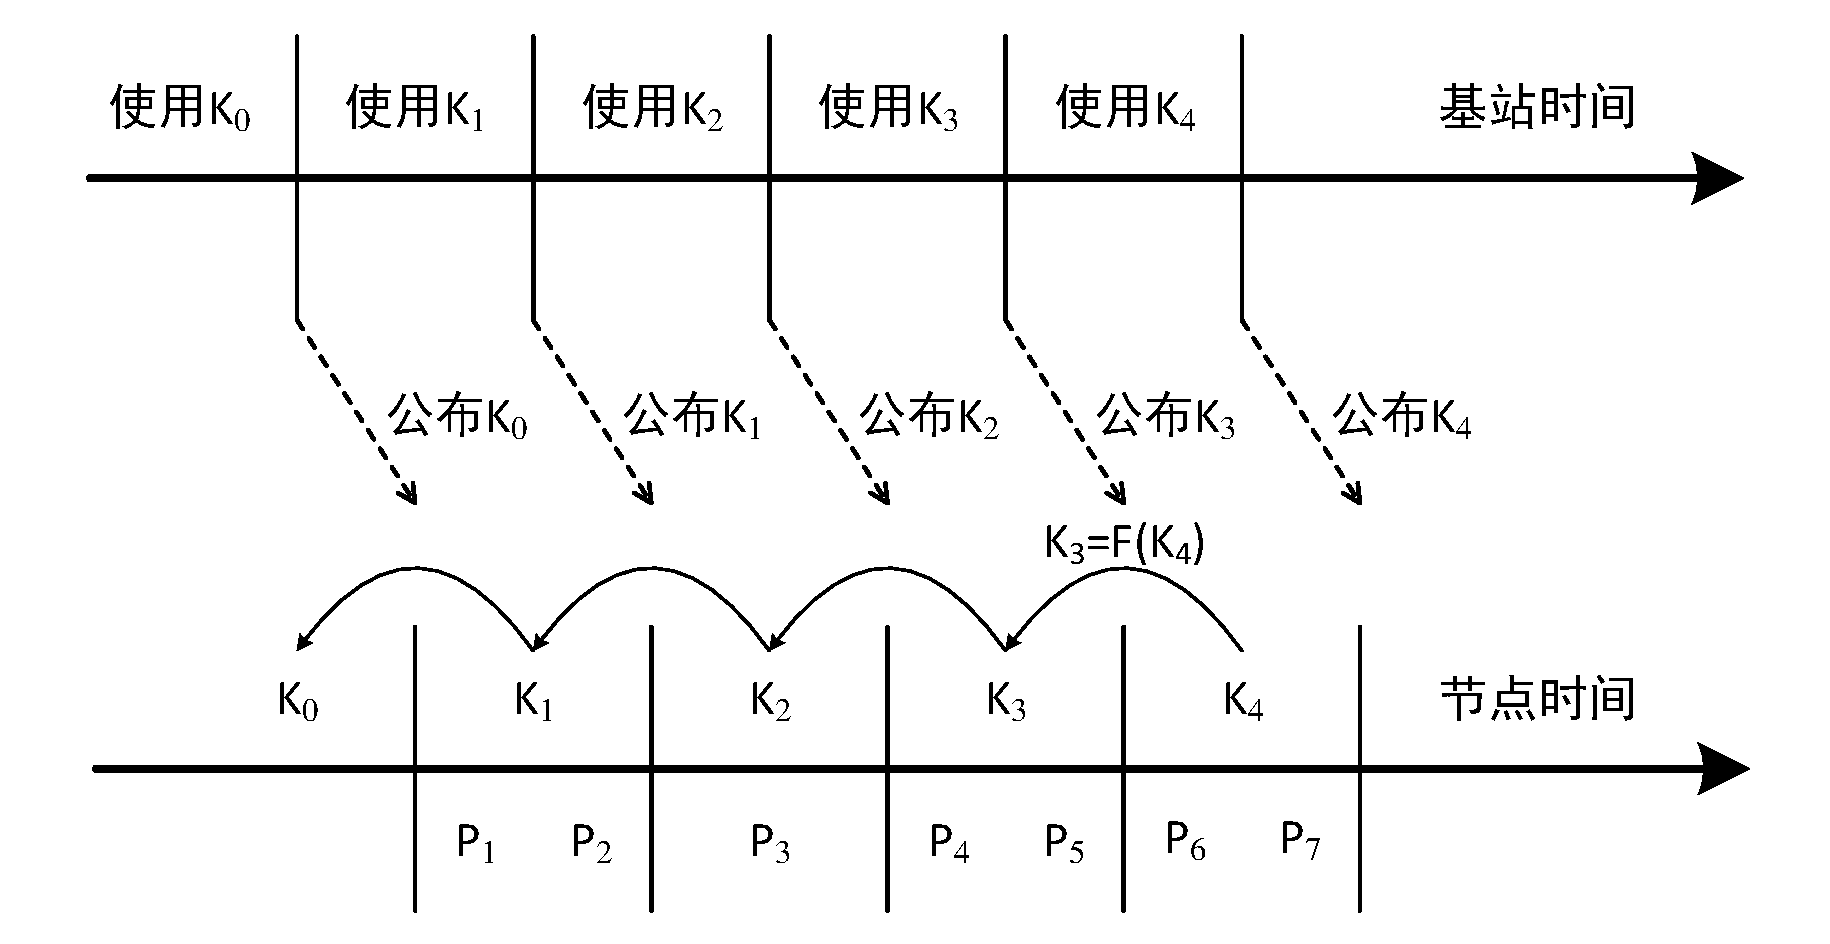
\includegraphics[width=5in]{TESLA}
  \caption{$\mu TESLA$认证机制}
  \label{fig:TESLA}
\end{figure}
如图~\ref{fig:TESLA}所示,是$\mu TESLA$方案的认证过程,$\mu TESLA$是基于对称密钥的,对报文计算消息认证码的认证密钥和节点对报文进行认证的密钥是相同的。其认证过程包括密钥建立、广播报文、自举接收者和对报文认证等步骤。其中密钥分发是通过单向hash 函数F 来实现的,如$K_3=F(K_4)$。 然后广播一个密钥$K_i$加密后的报文,无线传感网中基站和节点采用不同的时隙,使广播加密报文和接收到相应的密钥不同步。通过延迟发布密钥$K_i$,使得认证过程具有非对称性,提高认证的安全性能。通过比较报文的接收时间和认证密钥发布的时隙,能对报文的安全性进行检查。但该方案仍有其缺点:密钥的发布延后于报文的到达,因此节点接收到的报文必须缓存在节点中,浪费节点宝贵的存储空间,并且有可能被攻击者发动泛洪攻击,大量的伪造报文填满传感器节点的缓存空间,导致无线传感网传输功能失效,攻击者也容易发动虫洞攻击,威胁传感网的安全。

Liu等人基于$\mu TESLA$方案,提出了多级$\mu TESLA$方案\upcite{c1:MultiTesla},采用多级密钥链解决$\mu TESLA$方案中密钥链占用存储空间过大,容易导致泛洪攻击的问题。该方案使用预装初始化参数的方案,代替$\mu TESLA$方案中通过单播进行初始化的过程。如图~\ref{fig:MultiTESLA},是多级$\mu TESLA$方案的认证过程。在该方案中,Liu使用了2级时间,在1级时间中,将时间划分为$n_0$个间隔,每个时间间隔对应该级的单向hash链中的密钥$K_i,1\leq i \leq n_0$,其中密钥还是同$\mu TESLA$ 方案,使用单向hash链生成。一个1级时间间隔又被划分为$n_1$个2级时间间隔,每个2级时间间隔的密钥使用
$K_i,1\leq i \leq n_0$作为密钥种子生成。每个2级时间间隔内发送的报文用对应的密钥进行认证,其中的密钥链头$K_i,0$ 在前一个1级时间发布。
\begin{figure}[htbp]
  \centering
  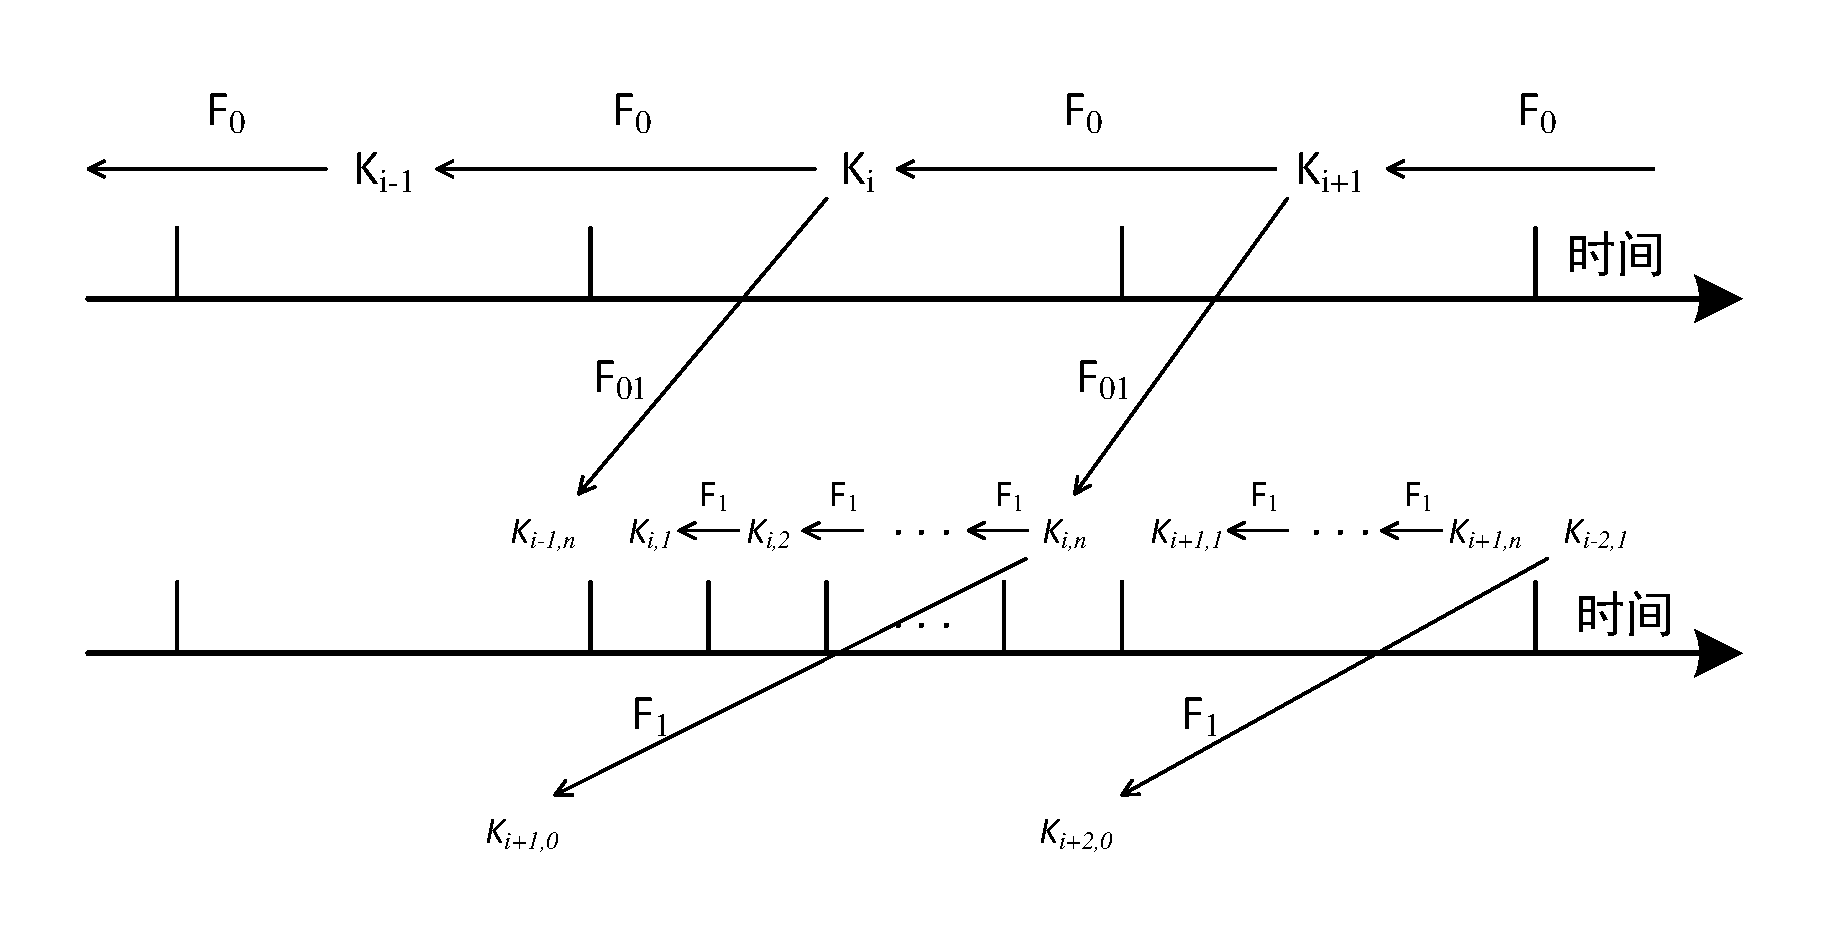
\includegraphics[width=5in]{multiTESLA}
  \caption{多级$\mu TESLA$认证机制}
  \label{fig:MultiTESLA}
\end{figure}

在裴庆祺等人的$\mu TESLA$改进方案中\upcite{c1:MMtesla},引入了$(t,n)$的门限秘密共享,每个认证密钥被分隔为$n$个密钥片,分配到各个基站。在无线传感网中执行原有的$\mu TESLA$方案,将密钥片进行广播,当一个节点接收到超过$t$个密钥片之后,就通过秘密共享的算法,对认证密钥进行恢复,重构出认证密钥。该方案提高了$\mu TESLA$方案的认证率,并且有高可靠性和高容忍性的特点,缺点是通信开销明显增加。

Anas等人提出了一种基于信任模型的认证方案\upcite{c1:anas},使用一个轻量级的基于椭圆曲线的简单认证密钥协议。通过通信实体之间建立信任级别,使非对称密钥认证系统能在资源有限的无线传感器节点上运行。

Dong等人利用消息预认证提出了一个基于密钥链的过滤方案\upcite{c1:verifyfilter},能对无线传感网中的广播进行过滤,有效减少虚假广播对传感网数据传输的影响,该方案的缺点是无法有效防御攻击者的联合节点攻击。




\subsection{无线传感网身份认证概述}

攻击者可以通过对网络发送大量的虚假数据报文,大量消耗节点的计算和存储能力,消耗节点的能量,导致传感网的失效。因此对传感网中的节点进行身份认证尤为重要。
文献\cite{c2:chan2003random}中,利用随机配对密钥分配方案,一个密钥仅会分配给一对节点,来实现一种非常简单的身份认证,即两个节点通过使用预分配的密钥对消息的加密和解密判断是否是经过认证的节点。但是该方案无法实现真正的身份认证,因为被捕获的节点可以伪装成正常节点进行欺骗,对无线传感网进行攻击。

现有的身份认证方案主要有非对称密钥认证和秘密共享认证。
由于无线传感器节点的限制,现阶段非对称密钥认证的实现一般是消耗能量较多的计算由基站完成,消耗能量较少的计算由节点完成。秘密共享的认证则是基于多个节点共同对一个节点进行认证。

虽然现阶段由于传感器节点的限制,非对称密钥没有被广泛应用于无线传感网的认证,但是许多研究也对此进行了探索。
在非对称密钥机制中,椭圆曲线密码(Elliptic Curve Cryptography,ECC)是一种轻量级的方案,研究结果表明,160位的ECC 能获得相当于1024位RSA密码的安全性能。而且使用非对称密钥不需要$\mu TESLA$方案中的延迟发布密钥,还能提高认证系统的安全性。

Watro等人提出了一个基于RSA算法的认证机制TinyPK\upcite{c1:Watro},该方案使用请求-应答机制。
该方案使用了双重校验,来保证认证机制的安全性。
当一个节点需要同另一个节点进行认证时,向该节点发送一个请求信息,其中包括两部分。第一部分是使用认证中心的私钥进行签名的请求节点的公钥,第二部分是使用请求节点私钥签名的时间戳和消息认证码。应答节点接收到该请求消息以后,使用认证中心的公钥对第一部分进行解密,获取请求节点的公钥。使用请求节点的公钥解密第二部分,获得时间戳和消息认证码,通过时间戳和消息认证码的校验,来判断请求节点的合法性。如果通过,则建立两个节点之间的安全通信。

在Bauer等人的方案\upcite{c1:Bauer}中,使用了秘密共享的思想进行身份认证。当一个节点请求对另一个节点的认证时,应答节点发送消息给认证中心,宣告自己被请求做认证处理,处理中心将请求节点的私钥进行划分,将秘密片广播给应答节点的邻居节点,所有节点发回给认证中心一个判定消息,如果通过认证的消息超过阈值,则请求节点通过认证,应答节点此时与认证中心进行交互,更新自己的私钥。

现有的身份认证方案还有Benenson提出的基于ECC的方案\upcite{c1:Benenson},Cao等基于vBNN-IBS提出的多用户广播认证方案\upcite{c1:Cao}。



\section{无线传感网密钥分配方案概述}

\subsection{无线传感网密钥分配概述}
无线传感网的密钥分配是其安全技术研究的一个重要内容,包括密钥预分发、共享密钥发现等研究方向。

无线传感网中的密钥分配与传统无线网络有较大区别,在传统的无线网络中,密钥分配方案的研究已经取得了许多成果,但是由于无法适应无线传感网的特点,这些成果无法应用于无线传感网中。因为WSN节点资源的限制,传统无线网络中节点计算开销和通信开销较大的密钥分配方案无法适用。在设计无线传感网的密钥分配方案时,不仅要保证方案的安全性能,也要权衡计算开销和通信开销。

进行认证的基础是密钥分配,设计一个面向无线传感网需求的密钥分配方案,才能保证认证机制的性能。
\subsection{无线传感网密钥分配方案分类}
近些年来,WSN的密钥分配有了许多新的研究成果,根据所适用的密钥是否是对称密钥,可以将方案分为对称密钥方案和非对称密钥方案。随着传感器技术的发展,非对称密钥技术可能成为将来无线传感器密钥分配的主流,但是由于目前无线传感器节点的计算能力和存储空间的限制,现有的无线传感网密钥分配以对称密钥方案为主。基于对称密钥,有很多的密钥分配机制的研究成果,表~\ref{tb:wsnkey}列出了目前无线传感网主要的密钥分配方案:

\begin{table}[htbp]
  \centering
  \caption{无线传感网主要的密钥分配方案}
  \label{tb:wsnkey}
  \begin{minipage}[t]{0.8\textwidth}
    \begin{tabularx}{\linewidth}{|c|X|X|}
      \hline
%      \multirow{1}*{网络层次}
%        & 常见的攻击 & 防范措施\\
      \multirow{1}*{数学结构}  & \multicolumn{1}{c|}{密钥分配方案} & \multicolumn{1}{c|}{密钥分配方法} \\
      \hline
      \multirow{3}*{密钥池}
        & E-G方案 & 随机预分发 \\\cline{2-2}
        & q-composite方案 & \\\cline{2-3}
        & PIKE方案 & 基于网格预分发\\
      \hline
      \multirow{4}*{二元对称多项式}
        & Blundo方案 & 确定预分发\\\cline{2-3}
        & Liu-Ning方案 & 基于随机子集预分发 \\\cline{2-3}
        & GBKP方案 & 基于网格预分发 \\\cline{2-3}
        & CPKS方案 & 基于位置预分发 \\
      \hline
      \multirow{2}*{MDS 码生成矩阵}
        & Blom方案 & 确定预分发 \\\cline{2-3}
        & Du-Deng方案 & 基于随机子集预分发 \\
      \hline
      \multirow{2}*{区组}
        & Camtepe方案 & 组合设计 \\\cline{2-3}
        & Camtepe混合组合设计方案 & 组合设计及随机预分发 \\
      \hline
    \end{tabularx}\\[2pt]
  \end{minipage}
\end{table}



\subsection{无线传感网典型密钥分配方案概述}
根据密钥分配方法的不同,我们对不同类别的无线传感网密钥分配方案进行概述:
\subsubsection{基于随机预分发的密钥分配}
Eschenauer和Gligor基于随机图理论,提出了无线传感网中随机密钥预分配的方案\upcite{c2:Eschenauer2002}(简称E-G方案),该方案包括3个阶段。在密钥预分发阶段,密钥分发中心生成一个足够大的密钥池$P$,然后对于每个传感器节点,从中随机选择$m$个不同的密钥,形成一个密钥环,并将密钥保存到传感器节点的存储空间中。在密钥发现阶段,每个节点通过相邻节点发现机制寻找物理上相邻的节点,由于所有节点的密钥是从密钥池中随机取出的,相邻节点可能存在相同的密钥,如果相邻节点存在共享密钥,则作为两者之间的会话密钥。当相邻节点之间不存在共享密钥,则开始路径密钥建立阶段。通过在密钥发现阶段建立的节点连通图$G(V,E)$(V为传感器节点的顶点集合,E为有共享密钥的传感器节点之间构成的边集),在图中查找一条通往没有共享密钥的相邻节点的路径,建立相邻节点之间的路径密钥。

在E-G方案中,两个相邻节点之间有共享密钥的概率$p$同节点存储密钥数$m$之间的关系可以表示为:$p=1-\frac{((P-m)!)^2}{(P-2m)!P!}$。E-G 方案使得每个节点只需要存储较小数量的密钥,就可以有较高概率使得无线传感器网络完成密钥建立过程,符合无线传感网的特点要求。但是E-G 方案作为最早提出的无线传感网密钥预分发方案,也有自身的缺点,当妥协节点增多时,无法保证无线传感网的通信安全,因为节点不具备防篡改的机制。而且当一个节点被捕获时,节点上存储的密钥材料全部都暴露给了攻击者,而且这些密钥可能是其他节点间的会话密钥,也就是使攻击者能攻击其他节点之间的通信。

在E-G方案的基础上,有许多方案对随机密钥预分配进行了改进,提升随机密钥预分配机制的性能。
Chan等人在E-G方案的基础上提出了q-composite 随机密钥预分配方案\upcite{c2:chan2003random},每个节点从密钥池$P$中获取$m$个不同的密钥。方案的密钥个数阈值为$q$,当两个节点之间的共享密钥个数$q^{'}$满足$q^{'}> q$,则两个节点之间使用hash函数$K=hash(K_1\| K_2\| \cdots \| K_{q^{'}})$生成会话密钥,在q-composite方案中,hash函数使用了SHA-1\cite{c2:sha1}。q-composite保证了相邻节点之间的安全链路,密钥个数阈值增大时,链路的安全性能也增大。在无线传感网被捕获节点较少时,该方案节点间链路的安全性能比E-G方案更好,但是当被捕获节点增多时,该方案的安全性能明显下降。


在Blom的对称密钥生成方案\upcite{c2:Blom84} 基础上,Du等人将其与随机密钥预分发结合,提出了无线传感网多密钥空间密钥预分发方案\upcite{c2:du2005pairwise}。先使用Blom方案生成$\omega$个密钥空间,每个节点从中选择$\tau$个密钥空间保证在存储空间中$(2 \leq \tau \leq \omega)$,如果两个节点上存储了一个相同的密钥空间,则他们之间计算生成一个共享密钥。与E-G 方案和q-composite方案相比,Du-Deng方案通过计算适合的参数$\omega$和$\tau$,能明显提高抵抗链路攻击的性能,但是同时也增加了节点的计算开销。

Blundo利用二元对称多项式的性质,提出了节点对密钥建立方案\upcite{c2:Blundo1998}。密钥服务器随机生成一个有限域上的$k$ 阶二元对称多项式$f(x,y)=\sum _{i,j=0}^k a_{i,j} x^i y^j$,对于对称多项式,有$f(x,y)=f(y,x)$。对于任意节点$i$,服务器计算$f(i,y)$,然后将$k+1$个系数存入节点存储空间。当节点$i$和节点$j$需要建立对密钥时,计算$f(i,y)$ 在$y=j$ 时的值,计算$f(j,y)$在$y=i$时的值,因为$f(i,j)=f(j,i)$,所以$f(i,j)$就可以作为节点$i$和节点$j$之间的对密钥。

在Blundo方案的基础上,Liu-Ning提出了基于对称二元多项式池的随机密钥预分配方案\upcite{c2:liu2005establishing}。
密钥服务器在有限域$F_q$上随机生成一个二元对称多项式的集合$\phi=\{f_i(x,y),i=1,\cdots,t\}$,对于节点$i$,将子集$\phi_i\subseteq \phi$装入存储空间。当两个节点发现有相同的二元多项式,则直接使用Blundo的节点对密钥建立方案建立会话密钥。当被捕获的节点较少时,Liu-Ning方案有较好的安全性能,但是在攻击者捕获了较多节点,也就是获得较多二元多项式的时候,链路的安全性能相较E-G方案和q-composite方案更低。

利用节点的位置信息,Liu提出了最近对密钥方案(CPKS)\upcite{c2:LiuN03},节点实际分布位置在其期望分布位置周围服从均匀分布。每个节点与自己期望分布位置最近的$t$节点之间建立对密钥,例如,对节点$u$的相邻节点$v$,密钥服务器生成对密钥$K_{u,v}$,并将$u,K_{u,v}$和$v,K_{u,v}$分别存入节点$u$和节点$v$。通过两个节点之间的ID信息可以判断两个节点之间是否存在对密钥。在节点位置信息已知时,该方案相比前述方案有更好的性能,缺点是网络扩展性较差,加入新节点,需要大量节点能量消耗。

Du提出的基于部署知识的方案\upcite{c2:Du06} 中,将密钥池$S$划分为$t\times n$的子密钥池$S_{i,j}(1\leq i\leq t,1\leq j\leq n)$,子密钥空间$S_{i,j}$对应着部署组$G_{i,j}$。根据部署位置的信息,不同的子密钥池之间发现共享密钥。该方案提高了无线传感网中节点链路连通的概率,但是子密钥池的划分对安全性能的影响较大。


\subsubsection{基于网格预分发的密钥分配}
为了解决随机密钥预分配方案中链路密钥的不确定性,Liu提出了基于网格的密钥预分配方案(GBKP)\upcite{c2:LiuND08}。
对一个$m\times n$的传感网,如图~\ref{fig:GBKP}所示,$G_i$为部署分组。对$G_i$中的节点分配ID集合$\{(i-1)m+j|j=1,\cdots,m\}$,对$G_i^{'}$中的节点分配ID集合$\{i+(j-1)m|i=1,\cdots,n\}$。服务器生成$m+n$个对称二元多项式分配给每行每列,使得同一行或同一列的节点能直接生成对密钥,不同行或列的节点,通过中间节点生成链路密钥。
类似的基于网格预分发的密钥分配方案还有Chan 提出的PIKE方案\upcite{c2:ChanP05}。
\begin{figure}[htbp]
  \centering
  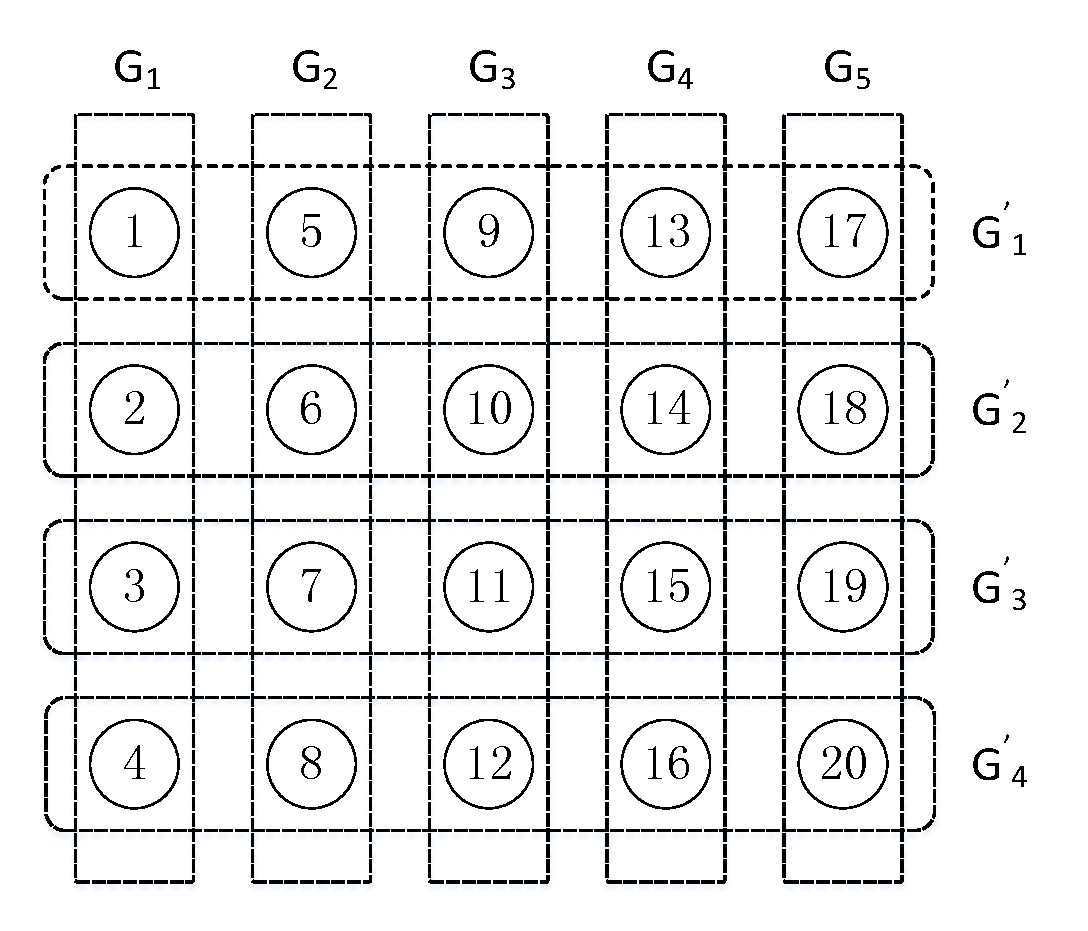
\includegraphics[width=4in]{GBKP}
  \caption{基于网格的密钥预分配方案}
  \label{fig:GBKP}
\end{figure}

\subsubsection{基于组合设计的密钥分配}
Camtepe把组合设计的理论应用于无线传感网的密钥分配\upcite{c2:CamtepeY07},使用组合设计理论来划分密钥池和密钥环。
对一个规模为$N$的无线传感网,生成一个对称BIBD,$(n^2+n+1,n+1,1)$,其中$n$为满足$n^2+n+1\geq N$的最小素数,密钥池的大小为$n^2+n+1$,密钥环的长度为$n+1$。这个方案保证了无线传感网中的任意一对节点有共享密钥,或通过中间节点生成的链路密钥。
为了解决该方案在网络规模方面的限制,Camtepe 还提出了组合设计与广义四边形想结合的方案。



\chapter{多跳长路径上多节点联合数据认证}
本章研究设计面向规模化无线传感网的多节点联合数据认证机制。
3.1节提出了多节点联合的数据认证模型和设计目标。
3.2节设计实现了多跳长路径上多节点联合的数据认证机制。
3.3节提出了面向3.2数据认证机制的路径上节点关系维护方案。

\section{无线传感网数据认证模型}

\subsection{无线传感网中数据认证场景}
无线传感网被广泛应用在环境监测、数据采集等领域中。如图~\ref{fig:wsn}所示是一个典型的无线传感网的应用场景,
在每个监测区域中,部署的传感器节点采集数据或感知事件后将数据发送给相应的簇头节点。簇头节点将接收到的数据进行
聚合之后,通过其与基站之间的若干传感器节点传输给基站。
\begin{figure}[htbp]
  \centering
  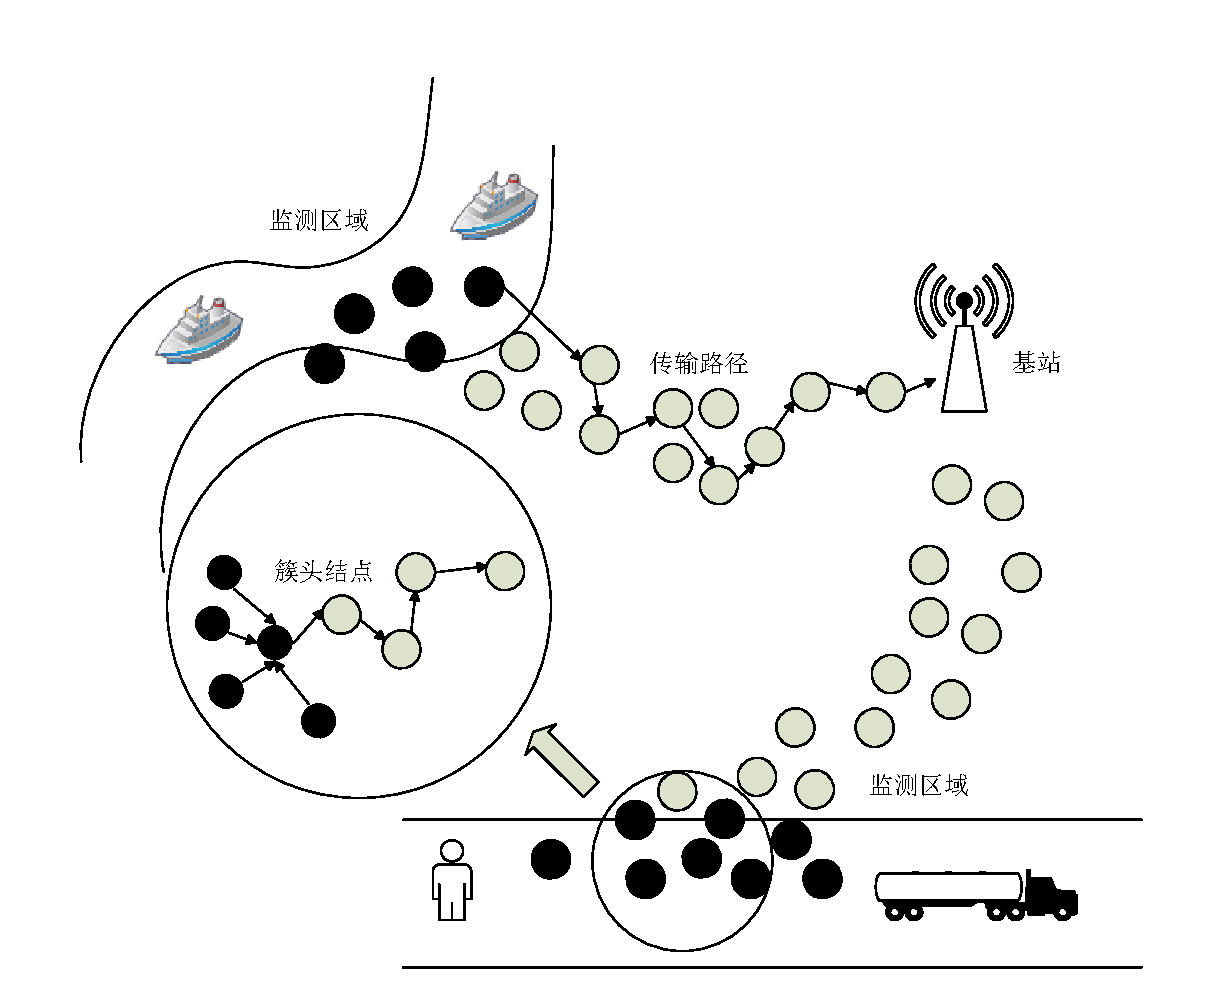
\includegraphics[width=5in]{wsnapp}
  \caption{无线传感网应用场景}
  \label{fig:wsn}
\end{figure}

无线传感网的认证包括传感器节点认证和数据认证,本文主要讨论数据认证。
传统的无线传感网认证方式是相邻节点,也即单跳之间利用预分配的密钥进行认证。由于无线传感器节点发射功率等的限制,
通信范围很小,攻击者很容易通过针对性地攻击或捕获节点,获取到密钥信息,从而攻破整个网络的认证系统。
利用预共享密钥密钥和节点信息生成节点间的共享对密钥,然后使用共享对密钥认证报文,能提高传感器网络的抗攻击的能力。

完全依靠广播传输机制,在大规模大数据无线传感网中,传输效率过低,消耗的传输能量和资源过大。有效利用大规模传感网中多跳长路径进行端对端数据传输,能够有效的保证传输效率。
%如果仅应用节点间的共享对密钥进行数据认证,路径中出现妥协节点时,整条路径的认证系统都会被攻破。
但是由于无线传感网部署环境恶劣、无人值守等原因,节点很容易被捕获或者被入侵,发送大量错误数据或垃圾数据,消耗传感器节点的能量,传统的认证机制无法对抗这种攻击。
本文研究的多节点联合数据认证机制,利用路径上多节点联合进行认证,能够有效地检测出垃圾报文,节约节点的能量。多节点联合数据认证通过维护传输路径上节点对之间的共享密钥,相隔多跳进行认证,有效提高认证系统抗攻击能力。

\subsection{多节点联合数据认证系统模型和设计目标}
\subsubsection{系统模型}
由于无线传感器节点的通信是基于广播的,所以攻击者很容易监听所有通信,注入虚假数据报文。本文假设当攻击者能够获得妥协节点的完全控制,可以获取节点中的所有密钥信息,并利用其发送虚假报文或者丢弃正常报文。攻击者的主要攻击手段是通过发送大量的虚假数据报文,达到消耗传感器节点能量的目的。
在本文的认证机制研究中假设攻击者能够有针对性地入侵节点,并利用妥协节点之间的联合来对抗认证机制。
%详述攻击模型

多节点联合数据认证的系统模型如图~\ref{fig:model}所示,主要由密钥分配、轻量MAC码和节点维护三部分组成。
\begin{figure}[htbp]
  \centering
  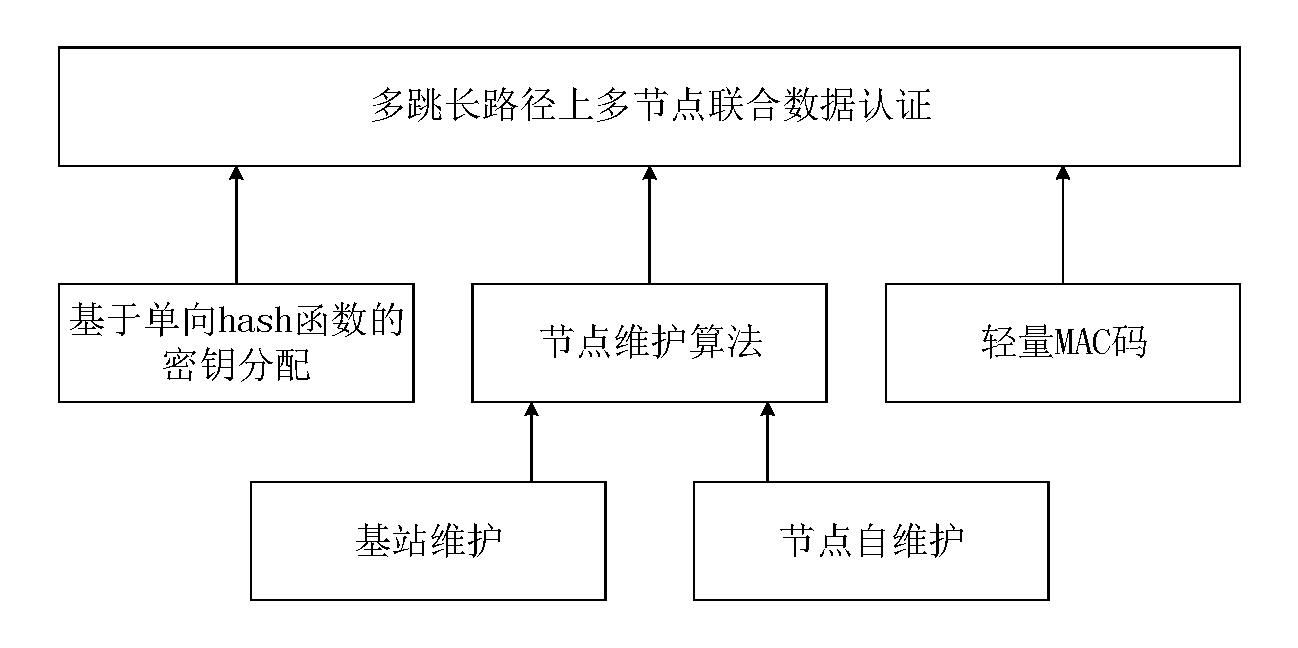
\includegraphics[width=5in]{model}
  \caption{多节点联合数据认证系统模型}
  \label{fig:model}
\end{figure}



本文中我们假设每个节点同基站之间都有共享密钥,而且每个节点都与它一跳内的相邻节点建立了对密钥,利用LEAP\upcite{c3:zhu2006leap}中提出的对密钥建立方案可以实现这个目标。
通过使用\upcite{c2:liu2005establishing,c2:du2005pairwise} 等密钥建立方案,
不相邻的节点之间可以建立对密钥,并在节点发现阶段获得对方的节点ID信息。簇与基站之间通过发现簇头之间的对密钥,形成多跳长路径,进行数据报文传输。

%添加关于簇头选举
%A Dynamic en-routing filtering scheme

\subsubsection{设计目标}
本章所研究的多跳长路径上多节点联合的数据认证机制包括如下设计目标:
\begin{enumerate}\setlength{\itemsep}{-\itemsep}
  \item 基站能够检测出所有虚假数据报文,保证传感网监测功能不受虚假报文的干扰。
  \item 当被入侵或捕获的节点数不大于t(t为系统设计参数)时,能保证虚假数据报文被丢弃。
  \item 传输路径注入的虚假数据报文,被检测并丢弃前经过尽量少的跳数,对于给定的t,我们的多节点联合认证系统有相应的虚假数据报文传播跳数上限。
  \item 认证机制计算高效,消耗能量小,适应无线传感网的要求。
  \item 能够有效应对节点失效,能够对传输路径上的节点关系进行维护,保证认证机制的稳定性。
\end{enumerate}

\section{多跳长路径上多节点联合的数据认证机制设计与实现}
\subsection{符号与定义}
本文中相关的符号定义如表~\ref{tab:notation}所示:
\begin{table}[htb]
  \centering
  \begin{minipage}[t]{0.8\linewidth} % 如果想在表格中使用脚注,minipage是个不错的办法
  \caption[相关符号说明]{相关符号说明}
  \label{tab:notation}
    \begin{tabular*}{\linewidth}{lp{10cm}}
      \toprule[1.5pt]
      {\hei 符号} & {\hei 描述} \\
      \midrule[1pt]
      $CN_i$ & 簇内节点 \\
      $t$ & 簇内节点个数,不包括簇头节点 \\
      $CH_i$ & 簇与基站之间长路径上的簇头节点\\
      $AK_{si}$ & ID为i的簇内节点与基站之间的共享密钥\\
      $AK_{uv}$ & 节点u与节点v之间的共享密钥\\
      $h_i$ & 簇头节点$CH_i$距离BS的跳数 \\
      $MAC(k,s)$   & 消息s通过密钥k生成的消息认证码\\
      \bottomrule[1.5pt]
    \end{tabular*}
  \end{minipage}
\end{table}

我们定义对于多跳长路径上的节点,当$|i-j|=t+1$时,$CH_i$和$CH_j$为相关节点。当$i-j=t+1$时,节点$CH_i$为节点$CH_j$的上行相关节点,节点$CH_j$为节点$CH_i$的下行相关节点。对于簇内节点,节点$CH_i$为节点$CN_i$的上行相关节点,节点$CN_i$为节点$CH_i$的下行相关节点。如图~\ref{fig:IHA1}所示,在$t=3$的簇与基站之间由8个簇头节点组成传输路径,其中$CN_3$为$CH_3$的下行相关节点,其中$CH_7$为$CH_3$的上行相关节点。
\begin{figure}[htbp]
  \centering
  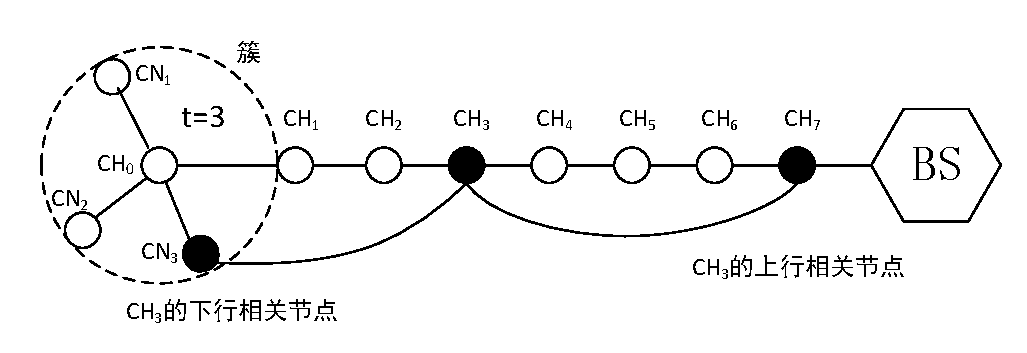
\includegraphics[width=5in]{IHA1}
  \caption{多节点联合数据认证中上下行相关节点}
  \label{fig:IHA1}
\end{figure}
\subsection{多节点联合数据认证方案}
我们的多跳长路径上多节点联合数据认证方案主要包括初始化、数据报文发送、路径中过滤、基站认证四个阶段。
\subsubsection{初始化}
传感器节点被部署到目标区域时会被分配唯一的ID和足够的密钥材料,保证每个节点与基站之间都有唯一的共享密钥$AK_{si}$。

在初始化阶段节点要获取上下行相关节点信息,在我们的多节点联合数据认证方案中,基站(Base Station,BS)会广播一个HELLO报文。簇头节点在收到HELLO 报文以后,保存$t+1$个ID信息作为上行节点,用自己的ID替换掉报文中距离自己$t+1$跳的节点的ID,其中被替换的ID信息作为其上行相关节点的ID,然后将报文继续广播。簇头节点会把该HELLO 报文中$t+1$ 个ID 分别发送给$t+1$ 个簇节点,包括簇头节点,这样每个节点都获得了上行相关节点的ID,并有了自己上行节点的ID信息。在接收HELLO报文以后每个簇头会节点记录下其到BS 之间的跳数。

簇头节点会向BS发送一个ACK报文,其中包括$t+1$个簇节点的ID。当簇节点的上行相关节点受到该ACK报文以后,保存下$t+1$个ID信息作为其下行相关节点,其中相距离自己$t+1$跳的节点的ID作为其下行相关节点ID,用自身的ID替换以后转发。BS收到ACK报文以后就建立了一条从簇到BS 的多跳长路径,而且各个节点都发现了其上下行相关节点的ID,并有了自己下行节点的ID信息。
\subsubsection{数据报文发送}
簇节点监测到事件E以后,必须要$t+1$个节点都发出报文才能确认监测到的事件,如果没有至少$t+1$个节点的报文,则认为是无效事件。

簇节点$CN_i(1\leq i\leq t)$对于事件E首先使用其与BS之间的共享密钥$AK_{si}$计算消息认证码$MAC(AK_{si},E)$,称其为簇节点MAC,并使用其与上行相关节点$CH_i$的共享密钥计算消息认证码$MAC(AK_{CN_i CH_i},E)$,称其为相关节点MAC。簇头节点$CH_0$ 从$t+1$个簇节点(包括簇头节点)收集到$t+1$份报文后对数据进行整合后发送。如图~\ref{fig:IHA2}所示,是一个事件E被感知和发送的过程。
\begin{figure}[htbp]
  \centering
  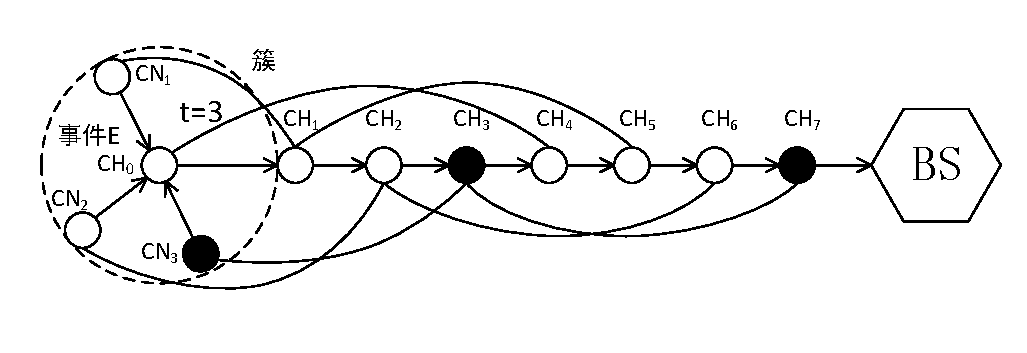
\includegraphics[width=5in]{IHA2}
  \caption{多节点联合数据认证中数据报文发送过程}
  \label{fig:IHA2}
\end{figure}

在图~\ref{fig:IHA2}的传输过程中,簇头节点$CH_0$收到簇节点的数据报文以后,对每个节点的簇节点MAC使用XOR运算进行压缩,缩小传输报文的大小,降低节点能量消耗,记作$XMAC(E)$:
\begin{equation}\label{XMAC}
\begin{split}
  XMAC(E)
  &=MAC(AK_{s1},E)\oplus MAC(AK_{s2},E)\oplus MAC(AK_{s3},E)\oplus MAC(AK_{s0},E)
\end{split}
\end{equation}
簇的ID记作$C_i$,簇头节点$CH_0$距离BS的跳数记作$h$,则对于事件E簇头节点$CH_0$发给BS的报文R可以记作:
\begin{equation}\label{report}
\begin{split}
  R=
  & E,h_0,\{CH_0,CN_1,CN_2,CN_3\},XMAC(E),\{MAC(AK_{CN_1 CH_1},E),\\
  & MAC(AK_{CN_2 CH_2},E),MAC(AK_{CN_3 CH_3},E),MAC(AK_{CH_0 CH_4},E)\}
\end{split}
\end{equation}
报文R中包含了簇节点的ID:$CH_0,CN_1,CN_2,CN_3$,从而BS能够认证压缩的$XMAC(E)$。

\subsubsection{路径中过滤}
当节点$CH_i$从下行节点收到报文R以后,首先用相邻节点共享密钥对进行认证。然后使用其上下行相关节点的共享密钥对E计算MAC,并更新报文R。对于图~\ref{fig:IHA2}中的节点$CH_1$,收到来自$CH_0$的报文后,使用与其下行相关节点$CN_1$之间的共享密钥对E 计算消息认证码$MAC(AK_{CH_1 CN_1},E)$,与报文R中的第$(h_0 - h_i)-((h_0 - h_i)/(t+1))\ast (t+1)=1$个相关节点MAC,$MAC(AK_{CN_1 CH_1},E)$ 进行比较,如果不同则丢弃报文R;如果相同,使用与其上行相关节点$CH_5$之间的共享密钥对E计算消息认证码$MAC(AK_{CH_1 CH_5},E)$,并替代原报文R中的$MAC(AK_{CN_1 CH_1},E)$,并将其转发给下一节点,更新后发送给节点$CH_2$的报文R为:
\begin{equation}\label{report}
\begin{split}
  R=
  & E,C_i,h_0,\{CH_0,CN_1,CN_2,CN_3\},XMAC(E),\{MAC(AK_{CN_1 CH_5},E),\\
  & MAC(AK_{CN_2 CH_2},E),MAC(AK_{CN_3 CH_3},E),MAC(AK_{CH_0 CH_4},E)\}
\end{split}
\end{equation}
\subsubsection{基站认证}
当BS收到报文R后,使用BS与报文R节点ID列表中$t+1$个簇节点之间的共享密钥计算MAC,并用XOR运算计算这$t+1$个MAC的值,与报文R中的XMAC比较,如果不同,则丢弃报文。如果相同,则对事件E作出响应。
\subsection{安全性能分析}
由于我们的方案使用了XOR运算压缩的XMAC保证了BS能检测出所有的错误报文,并且有相邻节点认证,下面我们对多节点联合认证的安全性能进行分析时,仅讨论路径中过滤的情况。

当一个节点被捕获时,攻击者就能获得一个能经过认证的MAC来欺骗它的上行相关节点。当传感器传输路径中被捕获的节点达到$t$个时,则攻击者可以用$t$个MAC组成的报文欺骗$t$个未被攻击的上行相关节点。但是我们的多节点联合数据认证机制需要$t+1$个有效MAC 才能通过认证,攻击者的入侵报文会被某个未被攻击的节点丢弃,因为它下行相关节点的MAC是无效的。因此我们的方案能保证当攻击者没有捕获超过$t$个节点的时候,入侵报文在被丢弃前仅能欺骗$t$个未被攻击节点。

通过上面的分析,我们的多节点联合数据认证机制的安全性是基于上下行相关节点间的认证的。我们下面对攻击者捕获了最多$t$个节点情况下的安全性进行分析,路径中过滤的攻击主要包括两个部分,簇内节点攻击和路径中节点攻击。
\subsubsection{簇内节点攻击}
当所有被攻击的$t$个节点都是簇内节点,没有路径中的节点被捕获时,不管簇头节点有没有被捕获,数据报文R中的$t+1$个MAC中总会有一个是无效MAC,从而被离簇头最近的$t+1$个路径节点(如图~\ref{fig:IHA2}中的节点$CH_1,CH_2,CH_3,CH_4$)中的某个检测出来并丢弃。
说明簇内节点攻击中,错误数据报文仅能欺骗最多$t$个未被攻击节点。

\subsubsection{路径中节点攻击}
我们讨论被攻击的$t$个节点在初始化阶段的ACK过程中能协作进行攻击的情况。我们讨论最坏情况,当被捕获的$t$个节点中包括了簇头节点$CH_0$,且从$CH_0$到BS之间间隔$t$个未被捕获节点均匀分布,可以表示为:
\begin{equation}
\begin{split}
  & CH_0,\{CH_{1,1},CH_{1,2},\cdots,CH_{1,t}\},N_1,\{CH_{2,1},CH_{2,2},\cdots,CH_{2,t}\},\\
  & N_2,\cdots,N_{t-1},\{CH_{t,1},CH_{t,2},\cdots,CH_{t,t}\},\cdots,BS
\end{split}
\end{equation}
其中$CH_0,N_1,N_2,\cdots,N_{t-1}$是被捕获的$t$个节点,任意两个被捕获节点被$t$个未被捕获节点分隔。

在初始化阶段,簇头节点$CH_0$在ACK阶段通过发送一个伪造的ID信息组,$y,CH_0,N_1,N_2,\cdots,N_t$,其中$y$为任意伪造的节点信息,使得上下行相关关系确定过程中,未被捕获节点的下行相关节点都为被捕获节点。由于间隔$t$个未被捕获节点之后,是一个被捕获的节点$N_i$,伪造的ACK 不会因为$y$是伪造的节点信息而被丢弃,而是重新将$y,CH_0,N_1,N_2,\cdots,N_t$转发给上行节点。完成了ACK过程以后,所有的未被捕获节点的下行相关节点都是被捕获节点。

簇头节点$CH_0$发送的错误数据报文R可以表示为:
\begin{equation}\label{report}
\begin{split}
  R=
  & E,C_i,h_0,\{CH_0,CN_1,\cdots,CN_t\},XMAC(E),\{MAC(AK_{N_t CH_1},E),\\
  & MAC(AK_{N_{t-1} CH_2},E),\cdots,MAC(AK_{CH_0 CH_t},E),MAC(AK_y,E)\}
\end{split}
\end{equation}
其中$MAC(AK_y,E)$为伪造的MAC。这个错误的数据报文能欺骗$t^2$个未被捕获节点,也就是攻击者捕获了最多$t$个节点时最坏的情况。
\section{路径上节点关系的维护方案}
我们的多节点联合数据认证机制是基于节点的上下行相关关系的,每个节点需要在初始化阶段发现其上行相关节点ID和下行相关节点ID,这样才能通过节点间的共享对密钥计算MAC,对数据报文进行认证。如果基站和簇头节点之间的多跳长路径是静态的,那只需要在初始化阶段进行一次上下行相关节点发现。但是由于无线传感网的特性,簇头节点在簇内是选举产生的,经常发生变化,还有传感器节点由于环境原因或者遭受攻击都有可能失效,导致路径的变化。因而需要对路径节点的上下行相关关系进行维护,以适应无线传感网的变化。下面从基站维护和节点自动维护两个情况介绍节点关系的维护。
%在拓扑结构变化不大的基础上。
\subsection{基站维护}
在相对稳定的无线传感网传输路径上,BS会周期性广播信标消息,信标信息中捎带每个节点的ID信息。
在初始化阶段,每个簇头节点都记录了自己到BS之间的跳数$h$。当一个节点收到信标消息以后,如果$h\geq t+1$,则检查该消息中$t+1$个上行节点的ID,如果$h< t+1$,则检查该消息中$h$个上行节点的ID。如果所有上行节点ID信息没有变化,路径中该节点的上行节点没有变化。如果有变化则在发送给BS的信标消息中附带节点变化消息,BS重新发送HELLO报文,进行上下行相关节点发现的过程。
\subsection{节点自动维护}
在基站维护的过程中,如果信标消息的广播周期较短,会造成大量的数据传输,消耗传感器节点的能量;如果信标消息的广播周期较长,那么部分节点失效或被攻击就会造成大量的数据报文被丢弃,所以我们需要节点自动维护的机制,修复路径中的节点上下行相关关系。
\begin{figure}[htbp]
  \centering
  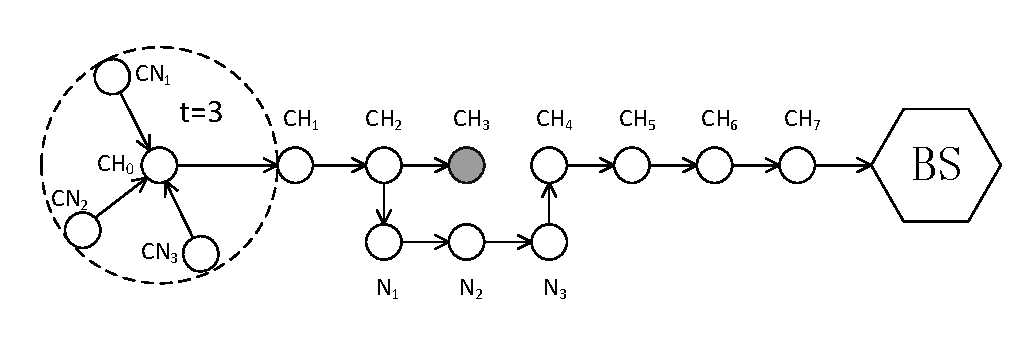
\includegraphics[width=5in]{IHA3}
  \caption{节点自动维护上下行相关关系的过程}
  \label{fig:IHA3}
\end{figure}

我们的节点自动维护机制是基于GPSR协议\upcite{c3:karp2000gpsr}中的右手准则的。我们假设每个节点都自动相邻节点的相对位置。如图~\ref{fig:IHA3}所示是一个节点自动维护的过程,当节点$CH_2$检测到$CH_3$失效以后,给它的逆时针方向的第一个相邻节点$N_1$ 发送一个修复消息,消息中包括了$CH_2$的$t$个上行节点的ID,$\{CH_4,CH_5,CH_6\}$,不包括$CH_3$。$N_1$,$N_2$按照初始化阶段的规则进行转发,当$N_3$收到修复消息以后,发现消息中有$CH_4$的ID,是它的相邻节点,这样就发现了一条替代路径。$N_3$将消息发送给$CH_4$以后,$CH_4$将上行节点ID,$\{CH_4,CH_5,CH_6,CH_7\}$捎带在消息中转发给$N_3$,同初始化阶段的HELLO报文。完成这些过程以后,新路径上的节点就建立上下行相关关系,也就是修复了这条长路径。

\section{本章小结}
本章提出了无线传感网中数据认证模型,针对相关攻击模型,提出了多跳长路径上多节点联合的数据认证方案。设计实现了多节点联合数据认证协议,并对其安全性能进行了分析。为了维持多节点联合数据认证机制的稳定性,设计了路径上相关节点关系维护的机制。



\chapter{数据认证方案优化}
本章介绍对第二章提出的多节点联合数据认证机制进行的优化,利用多种方案提升数据认证机制的检测效率,降低节点能量消耗。
4.1节介绍无线传感网节点失效问题,提出了多路径抗节点失效的机制。
4.2节设计动态步长的多节点联合数据认证机制对传感网能量开销进行优化。
\section{多路径抗节点失效机制}
\subsection{数据认证中的节点失效问题}
由于无线传感网部署的环境恶劣,且容易受到攻击,使得节点的稳定性很难保证,整个网络的拓扑结构很容易发生变化。在3.3节中,我们讨论了在拓扑结构变化频率不大的情况下,通过传感器网络自身的维护机制,维护路径节点的上下行相关关系,适应无线传感网拓扑结构的变化。但是在节点失效或者被攻击比较频繁时,无线传感器网络结构变化很快,而原有的维护方案是通过重建路径来完成的,因而通信开销较大,造成大量节点能量损耗。

为了适应节点失效较多,传感网拓扑结构变化较大的情况,我们提出了多路径抗节点失效的方案。通过在初始化阶段预定义若干条不相交路径,对每个节点失效的情况预定义编织路径。但在一个传输阶段,只有一条路径被使用,并进行数据认证。当路径受到攻击,或者节点失效时,使用备用的不相交路径或者编织路径。通过多路径抗节点失效机制,提升了传输路径的稳定性,保证了路径中检测虚假数据报文的性能。

在多路径抗节点失效方案中,我们使用了单向hash链来分配密钥,提升了网络的安全性能,并节省了节点存储密钥的开销。每个节点使用单向hash函数从它的上行相关节点的密钥生成密钥,具体的密钥分配方案将在第五章进行详细描述。
\subsection{多路径抗节点失效机制设计实现}
在多路径抗节点失效机制中,节点上下行相关关系不是研究重点,不再详细介绍,沿用第三章中多跳长路径多节点联合数据认证的方案。我们在多路径抗节点失效机制中,使用了单向hash链来分配密钥,能更好地保证认证机制的安全性,降低节点保存密钥的存储开销。我们的路径抗节点失效机制包括了初始化和密钥分配、数据报文发送、路径中过滤、基站认证、路径选择五个阶段,如图~\ref{fig:MPA}所示:
\begin{figure}[htbp]
  \centering
  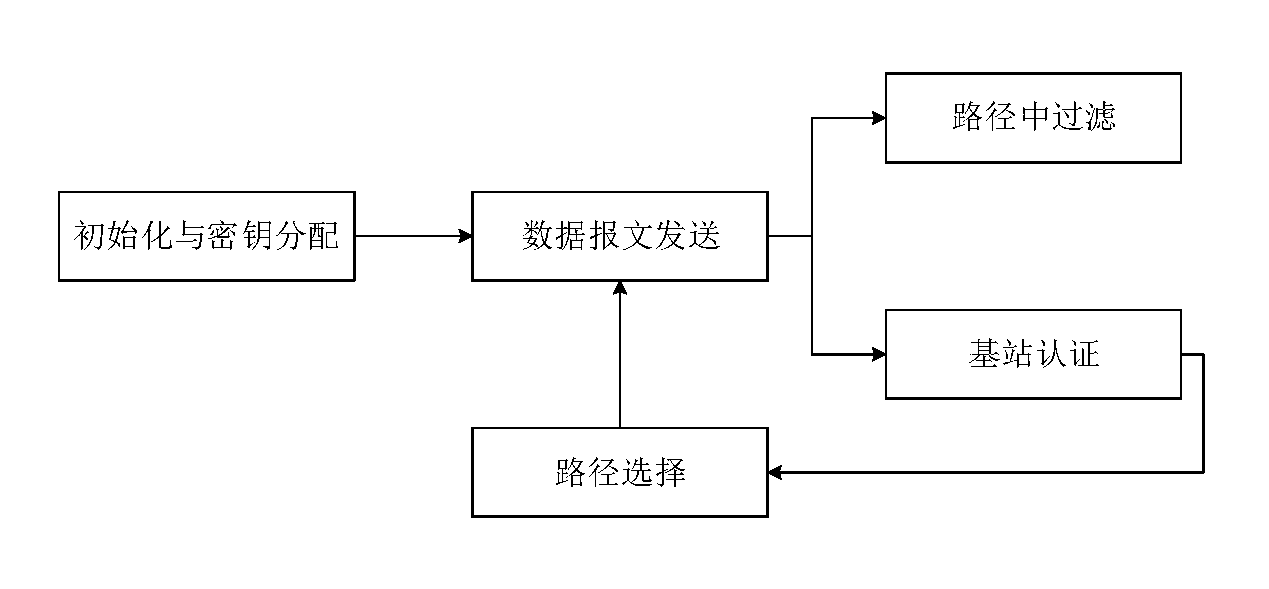
\includegraphics[width=5in]{MPA}
  \caption{多路径抗节点失效机制流程}
  \label{fig:MPA}
\end{figure}
\subsubsection{初始化和密钥分配}
传感器节点被部署到目标监测区域之后,基站会给每个节点生成一个共享密钥,这是每个节点与基站之间的共享密钥$AK_{si}$。然后每个簇通过预定的选举机制选举一个簇头节点,BS通过广播路由请求完成传感器网络的路由发现。

在多节点联合数据认证方案中,我们使用HELLO报文和ACK报文来完成路径发现和上下行相关关系的建立,在簇与BS之间建立一条多跳长路径。在多路径抗节点失效方案中,我们在初始化建立多条不相交长路径以及多条编织路径。虽然有多条路径,在我们的方案中,一次传输过程只会使用一条主路径,其他路径作为网络被攻击时的备选路径。

\begin{figure}[htbp]
  \centering
  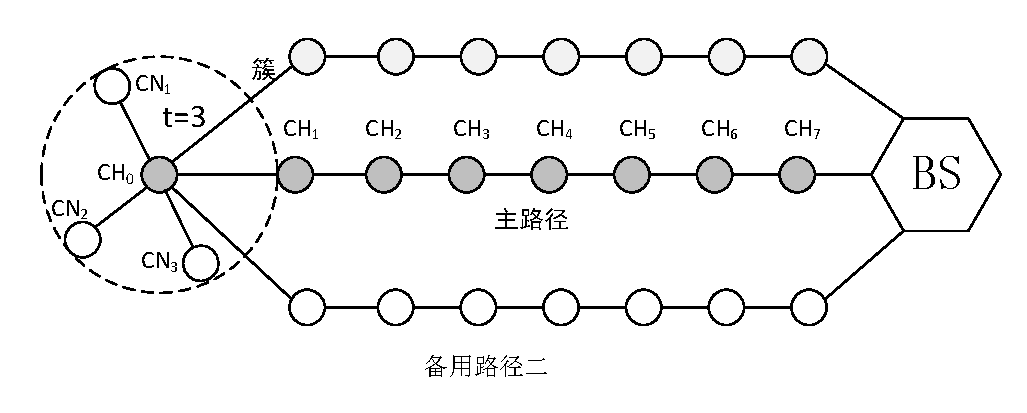
\includegraphics[width=5in]{IHAA1}
  \caption{多路径抗节点失效机制中的不相交路径}
  \label{fig:IHAA1}
\end{figure}
如图~\ref{fig:IHAA1}所示,簇与BS之间建立了3条不相交路径。不相交路径通过以下步骤建立:
\begin{compactitem}
  \item 建立一条簇头与BS之间的主路径。
  \item 建立一条与主路径不相交的,且跳数最短的路径,作为备用路径一。
  \item 建立一条与主路径以及备用路径一不相交的,且跳数最短的路径,作为备用路径二。
\end{compactitem}

\begin{figure}[htbp]
  \centering
  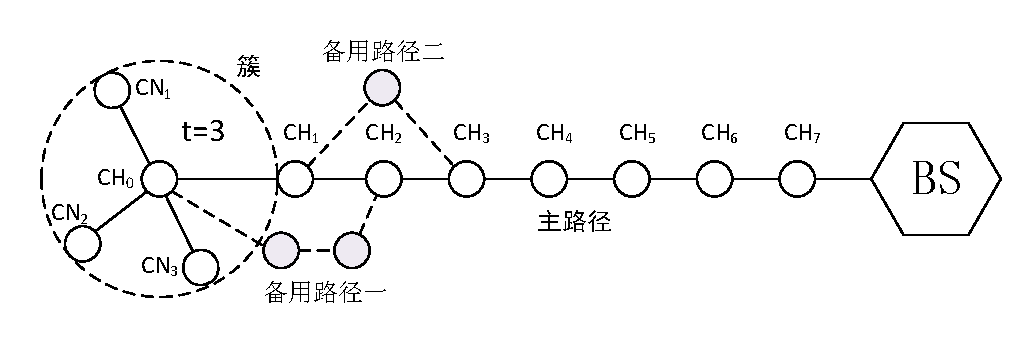
\includegraphics[width=5in]{IHAA2}
  \caption{多路径抗节点失效机制中的编织路径}
  \label{fig:IHAA2}
\end{figure}
如图~\ref{fig:IHAA2}所示,路径上的节点完成备用编织路径的建立。编织路径通过以下步骤建立:
\begin{compactitem}
  \item 建立一条簇头与BS之间的主路径。
  \item 对主路径上的每个节点,寻找不包括该节点的簇与BS之间的最短路径。在图~\ref{fig:IHAA2} 中,第一条编织路径就是不包括节点$CH_1$,从节点$CH_0$到节点$CH_2$之间的编织路径。相似的,第二条编织路径是不包括节点$CH_2$的从节点$CH_1$到节点$CH_3$的编织路径。
\end{compactitem}

\begin{figure}[htbp]
  \centering
  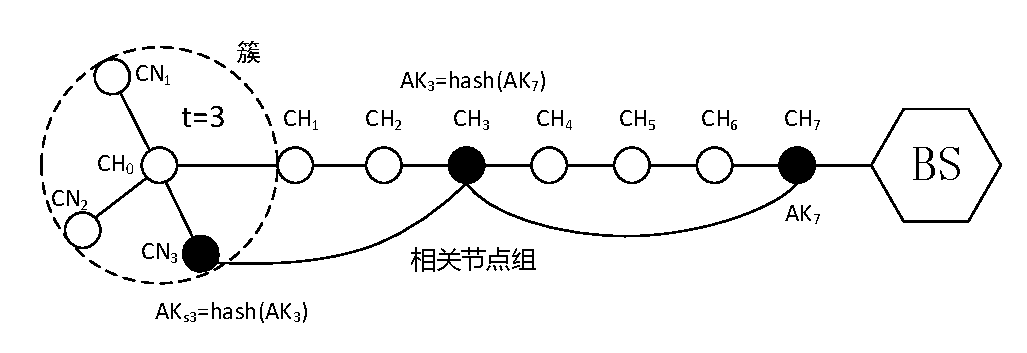
\includegraphics[width=5in]{IHAA3}
  \caption{多路径抗节点失效机制的密钥分配}
  \label{fig:IHAA3}
\end{figure}
在我们的多路径抗节点失效方案中,我们使用了单向hash链来进行密钥分配,如图~\ref{fig:IHAA3}所示。BS给每个上下行相关节点组生成一个$AK$,下行节点使用单向hash函数$H$从上行节点的密钥得到自己的密钥。图~\ref{fig:IHAA3}中所示,节点组\{$CN_3$,$CH_3$,$CH_7$\},距离BS最近的节点$CH_7$从BS获取BS生成的密钥$AK_7$,它的下行节点$CH_3$通过单向hash函数获取密钥$AK_3=H(AK_7)$。类似的,节点$CN_3$获取密钥$AK_{s3}=H(AK_3)$。通过这样的密钥分配,每个节点存储密钥的空间开销变小了,同时节点被攻击时丢失的密钥信息变少了。
\subsubsection{数据报文发送}
同多节点联合数据认证一样,簇节点监测到事件E以后,必须要$t+1$个节点都发出报文才能确认监测到的事件,如果没有至少$t+1$个节点的报文,则认为是无效事件。
簇节点MAC压缩后记作$XMAC(E)$:
\begin{equation}\label{XMAC}
\begin{split}
  XMAC(E)
  &=MAC(AK_{s1},E)\oplus MAC(AK_{s2},E)\oplus MAC(AK_{s3},E)\oplus MAC(AK_{s0},E)
\end{split}
\end{equation}
在多路径抗节点失效方案中,我们使用簇序号$C_i$来标记簇信息,代替原方案中的簇ID集,减小了传输开销。在簇头节点$CH_0$生成的报文R可以记作:
\begin{equation}\label{report1}
\begin{split}
  R=
  & E,C_i,h_0,XMAC(E),\{MAC(AK_{s1},E),\\
  & MAC(AK_{s2},E),MAC(AK_{s3},E),MAC(AK_0,E)\}
\end{split}
\end{equation}
\subsubsection{路径中过滤}
当节点$CH_i$从下行节点收到报文R以后,首先用相邻节点共享密钥对进行认证。然后使用其上下行相关节点的共享密钥对E计算MAC,并更新报文R。对于图~\ref{fig:IHAA3}中的节点$CH_3$,收到来自$CH_2$ 的报文后,首先使用单向hash函数计算得出其下行相关节点的密钥$AK_{s3}=H(AK_3)$。用$AK_{s3}$对事件$E$计算消息认证码$MAC(AK_{s3},E)$,与报文R中的第
$(h_0 - h_i)-((h_0 - h_i)/(t+1))\ast (t+1)=3$ 个相关节点MAC,也就是$MAC(AK_{s3},E)$进行比较,如果不同则丢弃报文R;如果相同则使用密钥$AK_3$ 对事件E计算消息认证码$MAC(AK_3,E)$,并替代原报文R中的$MAC(AK_{s3},E)$,将其转发给下一节点$CH_4$,更新后发送的报文R 为:
\begin{equation}\label{report2}
\begin{split}
  R=
  & E,C_i,h_0,XMAC(E),\{MAC(AK_1,E),\\
  & MAC(AK_2,E),MAC(AK_3,E),MAC(AK_0,E)\}
\end{split}
\end{equation}

\subsubsection{基站认证}
当BS收到报文R后,首先获取报文中的簇序号$C_i$,使用BS与簇$C_i$的节点ID列表中$t+1$个簇节点之间的共享密钥计算MAC,并用XOR 运算计算这$t+1$ 个MAC 的值,与报文R中的XMAC比较,如果不同,则丢弃报文。如果相同,则对事件E作出响应。
\subsubsection{路径选择}
当路径中节点受到攻击时,BS会收集到相应的信息,通过妥协节点检测技术\upcite{c4:mathews2007detecting},BS能确定哪些路径被攻击,妥协节点检测技术不是本文的重点,而是专注于妥协节点检测技术在数据认证中的应用。当BS确定了受攻击的路径以后,切换到未被攻击的备用路径。

同多节点联合数据认证机制中的节点关系维护相比,我们的多路径抗节点失效是通过预先定义备用路径,是一个应对节点攻击的前瞻性安全机制。而多节点联合数据认证机制中的节点维护是一种即时修复的方法,在节点失效或被攻击频率较高时,会造成传感器网络的传输路径不稳定,受攻击的影响更严重,还会造成大量的节点能量消耗。
\subsection{性能分析}
\subsubsection{安全性能分析}
在多跳长路径上多节点联合的数据认证机制中,被捕获节点的限度为$t$,当不少于$t$个节点被捕获,路径中的过滤就有可能无法检测出虚假数据报文。通过建立多跳备用路径和编织路径,多路径抗节点失效机制有更好的安全性能稳定性,在不少于$t$个节点被捕获时,仍能保证数据认证的安全性。

在多路径抗节点失效机制中,使用了基于单向hash链的密钥分配方案,保证了下行节点无法泄露上行节点的密钥。通过降低密钥信息丢失的概率,也提升了数据认证机会的安全性能。
\subsubsection{开销分析}
簇规模为$t+1$时,多路径的建立需要最少$N=(t+1)+d(t+1)$个节点,编织路径的建立需要至少$2(t+1)$个节点。
在提出的多路径抗节点失效机制中,MAC的计算是主要的计算开销,而且多路径抗节点失效机制中,每个节点进行认证前需要使用hash 函数进行密钥计算,使用SHA-1进行2byte的hash函数运算需要$1.52 \mu J$的能量开销。多路径抗节点失效机制需要维护多条备用路径和编织路径,有更高的能量开销,但是在虚假数据报文的比例较高时,因为其稳定的检测率,能明显减小传感网的能量开销。

\section{动态步长多节点联合数据认证}
\subsection{数据认证中的传输开销问题}
在无线传感网的多跳长路径传输中应用我们的多节点联合数据认证机制,能有效保证数据的安全传输,但是数据报文中附带了大量的MAC信息,加重了传感器节点的能量消耗。在规模化无线传感网中,由于传输路径跳数较多,数据传输实时性较高,节点的能量开销较大,因此安全机制的开销优化非常重要。

我们提出了一个动态步长的多节点联合数据认证,在传感器网络节点受攻击影响较小的时候,压缩所传输的报文,降低节点能量消耗,优化无线传感网的开销。
\subsection{动态步长多节点联合数据认证机制设计}
动态步长多节点联合数据认证是在多节点联合数据认证的基础上,对其进行改进,使得通信开销得到优化。
在4.1节中,我们讨论了在传感网拓扑结构变化较大时,使用多路径抗节点失效的机制来保证传感网传输稳定性。对于一条簇到BS之间的传输路径,如果路径比较稳定,则可以通过压缩数据报文的方式来降低传输开销。在我们提出的动态步长多节点联合数据认证机制中,是通过动态调整多节点联合认证中的节点组间隔步长来实现的。

在多节点联合数据认证中,根据步长的动态调整,对数据报文中的相关节点MAC进行相应程度的压缩处理,在路径传输的安全性与路径传输通信开销之间进行平衡,在保证路径安全性的情况下,降低通信开销。如图~\ref{fig:IHAA4}所示,是一个簇节点数为4,步长为3 的多节点联合数据认证。
\begin{figure}[htbp]
  \centering
  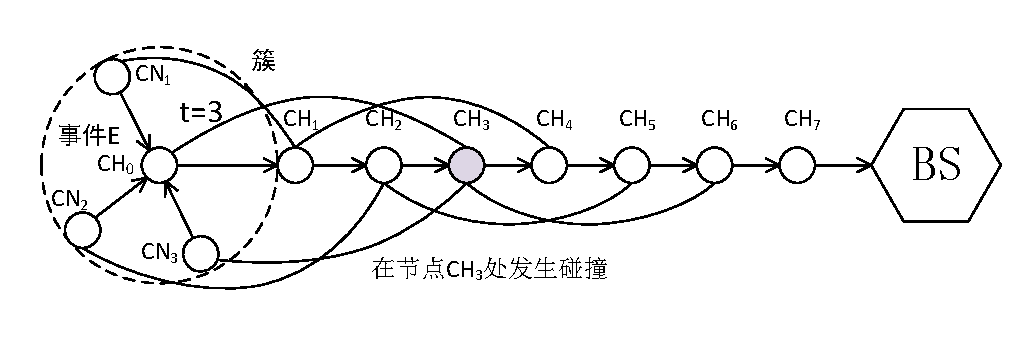
\includegraphics[width=5in]{IHAA4}
  \caption{动态步长多节点联合数据认证}
  \label{fig:IHAA4}
\end{figure}
\subsubsection{面向动态步长多节点联合数据认证的密钥分配}
%密钥分发,节点关系
在动态步长多节点联合数据认证中,我们也使用单向hash链来完成认证密钥的分配。不同于图~\ref{fig:IHAA3}中所示的密钥分配,在步长动态变化时,上下行相关节点组会发生碰撞,也就是不同的簇节点在同一个上下行相关节点组当中。如图~\ref{fig:IHAA4}中,节点$CH_0$和节点$CN_3$在同一个上下行相关节点组中,上行相关节点都是节点$CH_3$。

对于上下行相关节点的碰撞,我们通过对簇内节点添加虚拟的上下行顺序来解决。在如图~\ref{fig:IHAA4}的传输路径上,将4个簇节点的虚拟上下行关系设为$\{CN_3,CN_2,CN_1,CH_0\}$,也即步长为3时,节点$CH_0$是节点$CN_3$的上行相关节点。

\begin{figure}[htbp]
  \centering
  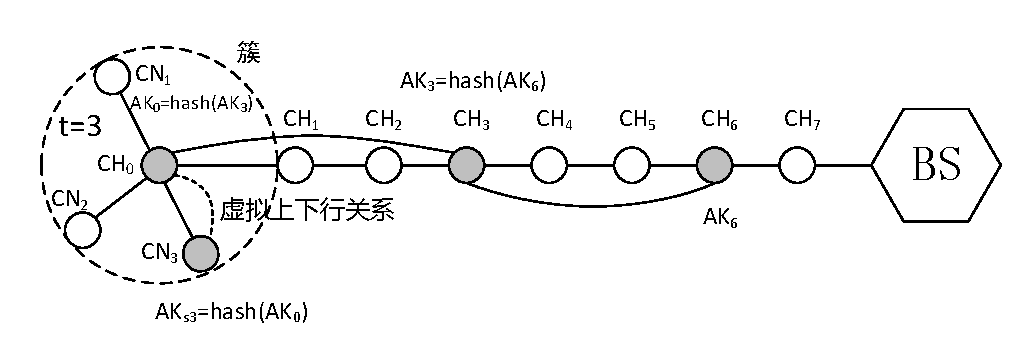
\includegraphics[width=5in]{IHAA5}
  \caption{面向动态步长多节点联合数据认证的密钥分配}
  \label{fig:IHAA5}
\end{figure}

如图~\ref{fig:IHAA5}所示,即为图~\ref{fig:IHAA4}所示的动态步长多节点联合数据认证情景的密钥传输示例。节点$CH_0$和节点$CN_3$都是簇节点,但是在同一个上下行相关节点组内,所以在节点$CH_0$和节点$CN_3$之间虚拟上下行相关关系,节点$CN_3$的密钥从节点$CH_0$的密钥计算而来,$AK_{s3}=H(AK_0)$。
\subsubsection{报文数据压缩传输}
使用单向hash链的密钥分配方案,给虚拟上下行相关节点分配了密钥以后,如图~\ref{fig:IHAA4}的动态步长多节点联合数据认证中,节点$CH_0$ 对簇节点数据进行整合之后的报文R可以表示为:
\begin{equation}\label{report3}
\begin{split}
  R=
  & E,C_i,h_0,XMAC(E),\{MAC(AK_{s1},E),MAC(AK_{s2},E),\\
  & MAC(AK_0,E)\oplus MAC(AK_{s3},E)\}
\end{split}
\end{equation}
其中$MAC(AK_0,E)\oplus MAC(AK_{s3},E)$为节点$CH_0$和节点$CN_3$的簇节点MAC使用XOR运算压缩后的结果。

我们用$p$表示步长,对于$h-h_0\leq p$的节点,在收到报文后,首先计算其下行相关节点的密钥。在图~\ref{fig:IHAA4}的示例中,节点$CH_3$ 收到报文R以后,首先计算下行相关节点的密钥$AK_0=H(AK_3)$。对事件E计算消息认证码$MAC(AK_0,E)$,并与报文R中第
$(h_0 - h_i)-((h_0 - h_i)/p)\ast p=3$个MAC进行比较,如果相同则用$MAC(AK_3,E)$替换之。如果不同则计算间隔一跳的下行相关节点的密钥$AK_{s3}=H(AK_0)$,对事件E计算消息认证码$MAC(AK_{s3},E)$,并与$MAC(AK_0,E)$进行XOR运算,
$MAC(AK_0,E)\oplus MAC(AK_{s3},E)$与报文R中第3个MAC进行比较,如果相同则用$MAC(AK_3,E)$替换之。
如果都不同,则表示是错误数据报文,但是不同于前面提出的方案,我们不将其直接丢弃,而是将$XMAC(E)$置为全0。
对于$h-h_0> p$的节点,同前述方案一样,只进行一次MAC验证。
在经过路径节点的验证后,节点将报文继续转发给上行节点。

\subsubsection{动态步长调整机制}
在BS收到报文以后,会对报文中的$XMAC(E)$进行验证。如果$XMAC(E)$为全0,则说明有错误数据报文在路径中被检测出来,这样说明传输路径的安全水平较低,则BS提高路径的传输步长$p$,这样能提升检测出错误数据报文的概率。如果BS连续收到若干个正常,达到一个阈值以后,我们认为路径是安全的,则BS降低路径的传输步长$p$,减小报文的大小,节约节点的传输能量。
\subsection{性能分析}
动态步长调整机制是建立在基站对路径的安全水平的评价基础上的,当路径的安全水平较高时,调整步长,压缩数据报文大小,降低传输的能量开销;当路径安全水平较低时,维持原有的步长,保证数据认证的安全性能。因此动态步长数据认证机制在安全性能上相比多节点联合数据认证无明显降低。

动态步长数据认证机制有效的在安全性能和能量开销之间进行权衡,在保证基本的安全性能的基础上优化能量开销。
在传感网中的虚假数据较少,也就是路径安全水平较高时,动态步长数据认证机制在能量开销上有明显的优化。

\section{本章小结}
本章针对多节点联合数据认证机制中,节点失效或者受攻击对路径中的节点相关关系的影响,我们提出了多路径抗节点失效的机制,设计实现了相关算法。为了优化多节点联合数据认证的通信开销,我们设计实现了动态步长多节点联合数据认证机制。对两个优化方案,都进行了相关安全性能的分析。




\chapter{密钥分配与消息认证码的实现}
本章首先讨论数据认证机制中的密钥分配方案,以及认证过程中使用的消息认证码的实现。在6.1中基于单向hash链的思想,设计实现了面向数据认证机制的密钥分配方案。在6.2节中设计了适应无线传感网认证需求的MAC码。

\section{面向数据认证的密钥分配方案}
在本节中我们讨论研究单向hash链的性质,并将其应用到密钥分配中,设计基于单向hash链的的密钥分配机制。

我们对本章中出现的符号的定义如表~\ref{tab:macnotation}所示:
\begin{table}[htb]
  \centering
  \begin{minipage}[t]{0.8\linewidth} % 如果想在表格中使用脚注,minipage是个不错的办法
  \caption[消息认证码相关符号定义]{相关符号定义}
  \label{tab:macnotation}
    \begin{tabular*}{\linewidth}{lp{10cm}}
      \toprule[1.5pt]
      {\hei 符号} & {\hei 描述} \\
      \midrule[1pt]
      $|\mathbf{K}|$ & K的长度 \\
      $<i>$ & 表示将整数$i$用$b$位二进制表示\\
      $\mathbf{A}\|\mathbf{B}$ & 将字符串A与B进行串联 \\
      $E_K(M)$ & 对消息M使用密钥K进行分组密码置换\\
      $A\ll i$ & 将字符串A左移i位,右边填0\\
      $\mathbf{A} \oplus \mathbf{B}$ & 将字符串A与字符串B按位异或\\
      \bottomrule[1.5pt]
    \end{tabular*}
  \end{minipage}
\end{table}
\subsection{单向hash链}
本节中的密钥分配方案是基于单向hash函数的特性来保证无线传感网中的密钥安全的。通过使用单向hash链生成密钥池,能保证在密钥部署时的安全需求,还可以通过建立节点间的通信密钥有效防止攻击者通过身份冒充对节点间通信攻击。我们对单向hash链的定义以及本文方案中选取的单向hash函数进行说明。
\subsubsection{单向hash链的定义}
hash函数是通过压缩映射将任意长度的消息压缩为一个固定长度的摘要的函数。
对一个任意大小的消息,hash函数能输出一个给定长度的散列值,一个hash函数$H$可以表示为$H:\{0,1\}^*\rightarrow\{0,1\}^i$,其中$i$ 为输出的散列值的长度。
满足下列条件的hash函数称作单向hash函数:
\begin{enumerate}\setlength{\itemsep}{-\itemsep}
  \item hash函数$H(x)$的输入$x$为任意长度
  \item hash函数$H(x)$的输出为给定长度
  \item hash函数$H(x)$的计算方便,也就是对于一个给定的输入$x$,hash值输入$y=H(x)$的计算是方便的
  \item 对于给定的hash值$y=H(x)$,找出$x$在计算上是不可行的
  \item 对于给定的输入$x$,找出另一个消息$x^{'}\neq x$,满足$H(x^{'})=H(x)$在计算上是不可行的
  \item 找出任意两个消息$x$和$y$,满足$H(x)=H(y)$在计算上是不可行的,也就是$H(x)$具有抗碰撞性
\end{enumerate}



通过对一个字符串种子$K_0$使用hash函数进行迭代,形成一个字符串链,称作hash链。如果使用的hash函数是单向hash函数,则hash链称作单向hash链,链中的字符串具有不可逆计算的特性。
例如对于单向hash函数$H(x)$,通过$K_{i+1}=H(K_i),0\leq i < n$迭代生成的单向链$K_0,K_1,\cdots,K_n$就是一个单向hash链。

\subsubsection{单向hash函数的选择}
典型的单向hash函数有SHA-1或者RC5等,可以通过将算法简化,使之适应无线传感网的需求。
在SHA-1方案中,输入是最大$2^{64}$bit的消息,输出是固定160bit的消息摘要。
我们的方案中将SHA-1的输出改进为64bit(也就是我们的数据认证机制中的密钥长度),作为我们的单向hash链生成函数。

改进后的基于SHA-1 的单向hash函数算法可以表示为算法~\ref{alg:sha-1}:
\begin{algorithm}[htbp]
  \caption{单向hash函数}
  \label{alg:sha-1}
  \begin{algorithmic}[1]
    \REQUIRE 输入消息$x,|x|=64$
    \ENSURE 消息摘要
    \STATE $M \leftarrow x\| 1\| 0^t\| <|x|>$,将消息x填充为512位
    \STATE 将消息M分隔为$w_0,w_1,\cdots,w_{15}$
    \STATE $A \leftarrow h_0 = 0x67452301$
    \STATE $B \leftarrow h_1 = 0xEFCDAB89$
    \STATE $C \leftarrow h_2 = 0x98BADCFE$
    \STATE $D \leftarrow h_3 = 0x10325476$
    \STATE $E \leftarrow h_4 = 0xC3D2E1F0$
    \FOR{$i=16$ to $79$}
        \STATE $w_i \leftarrow (w_{i-3}\oplus w_{i-8}\oplus w_{i-14}\oplus w_{i-16})\ll 1$
    \ENDFOR
    \FOR{$i=0$ to $79$}
        \STATE $temp \leftarrow A\ll 5 + f(B,C,D)+E+w_i+K_i$
        \STATE $E \leftarrow D$
        \STATE $D \leftarrow C$
        \STATE $C \leftarrow B\ll 30$
        \STATE $B \leftarrow A$
        \STATE $A \leftarrow temp$
    \ENDFOR
    \STATE $A \leftarrow h_0+A$
    \STATE $C \leftarrow h_2+C$
    \RETURN $A||C$
  \end{algorithmic}
\end{algorithm}

\subsection{基于单向hash链的密钥分配}
在第四章中已经简要介绍了多路径抗节点失效中的密钥分配,在这节中对我们的基于单向hash链的密钥分配方案进行详细论述。主要分为四个部分,分别是密钥预分配、共享密钥发现、路径密钥发现和密钥分配的扩展性。
\subsubsection{密钥预分配}
在传感器节点被部署到目标监测区域之前,每个节点预先装配了足够了密钥材料,包括节点的ID信息,以及单向hash函数H(在上节中已经详细论述)。基站基于单向hash函数H生成预分配密钥池:
\begin{equation}
  K_{i,j}=H^{1}(K_{i-1,j})=\cdots=H^{i}(K_{0,j})\quad (i=1,2,\cdots,n)
\end{equation}

其中$j$为单向hash链的序号,$n$代表单条hash链中的密钥个数,$H^{i}(K_{0,j})$代表密钥$K_{0,j}$经过$i$次hash函数的迭代。
将每条hash链上的密钥反序排列,得到的hash链序列为$K_{i,j},\cdots,K_{1,j},K_{0,j}$。基站共生成$m$条单向hash链作为密钥池,则整个预分配密钥池可以如表~\ref{tab:hashline}表示:

\begin{table}[htb]
  \centering
  \begin{minipage}[t]{0.8\linewidth} % 如果想在表格中使用脚注,minipage是个不错的办法
  \caption[预分配密钥池]{预分配密钥池}
  \label{tab:hashline}
    \begin{tabular*}{\linewidth}{c}
      \toprule[1.5pt]
        $\quad \quad K_{n,1}\quad -\quad K_{n-1,1}\quad -\quad \cdots\quad -\quad K_{2,1}\quad -\quad K_{1,1}\quad -\quad K_{0,1}$\\
        $\quad \quad K_{n,2}\quad -\quad K_{n-1,2}\quad -\quad \cdots\quad -\quad K_{2,2}\quad -\quad K_{1,2}\quad -\quad K_{0,2}$\\
        $\quad \quad K_{n,3}\quad -\quad K_{n-1,3}\quad -\quad \cdots\quad -\quad K_{2,3}\quad -\quad K_{1,3}\quad -\quad K_{0,3}$\\
        $\quad \quad \cdots$\\
        $\quad \quad K_{n,m}\quad -\quad K_{n-1,m}\quad -\quad \cdots\quad -\quad K_{2,m}\quad -\quad K_{1,m}\quad -\quad K_{0,m}$\\
      \bottomrule[1.5pt]
    \end{tabular*}
  \end{minipage}
\end{table}

部署节点时,预分配的密钥从密钥池中取出,分配给节点。最先被分配的密钥是密钥池中靠前的密钥集合,也即密钥集合$K_{n,1},K_{n,2},K_{n,3},\cdots,K_{n,m}$最先被分配,后续部署到无线传感网中的节点依次从预分配密钥池中取出密钥集合进行分配。通过这样的预分配方式,不同阶段部署的节点使用的不同的密钥集合中的密钥,限制了被攻击节点泄露的密钥对整个无线传感网的影响,攻击者不能对已经建立的安全通信链路进行攻击。由于密钥池是一系列的反序单向hash 链,单向hash链的特性决定了泄露的密钥无法推导出密钥池中的密钥,因此攻击者无法进行节点冒充攻击。

\subsubsection{共享密钥发现}
节点被部署到目标区域以后,利用相应的分簇算法,对网络结构进行组织,选举每个簇的簇头。在簇的建立完成以后,节点之间开始共享密钥发现的过程。

在第二章中,我们已经讨论过密钥预分配方案的缺点,当节点被攻击而成为妥协节点时,节点中的预分配密钥都会被攻击者获得,可以对无线传感网的通信进行攻击。因此我们需要在节点之间发现相同的预分配密钥,并生成节点对之间的共享密钥。建立共享密钥的过程如图~\ref{fig:keyACK}所示:
\begin{figure}[htbp]
  \centering
  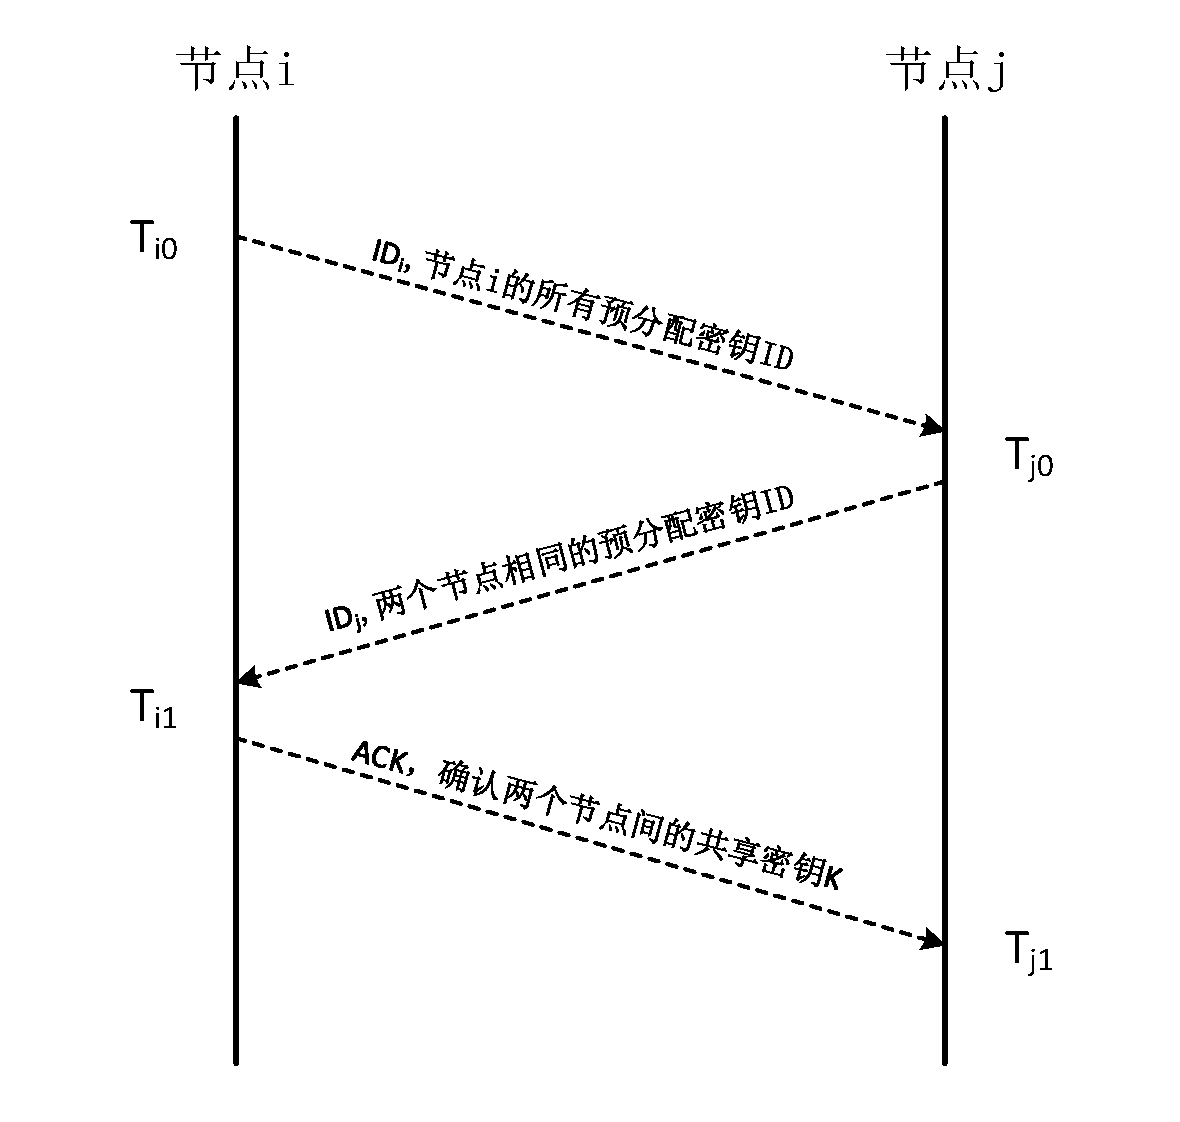
\includegraphics[width=5in]{keyACK}
  \caption{共享密钥建立过程}
  \label{fig:keyACK}
\end{figure}

节点部署到目标区域到网络进行初始化阶段的时间内,假设网络是不受攻击的影响,节点不会被攻击或者被捕获,能安全进行信息的交换。
相邻的节点i与节点j之间发现共享密钥的过程是先由节点i将其节点ID以及所有预分配密钥的ID一起广播。节点j收到邻居节点的ID以及预分配密钥ID以后,在自己的预分配密钥中进行寻找,如果有相同的预分配密钥$K_x$,则将自己的ID以及相同的预分配密钥ID一起发送给节点i。节点i在受到节点j的节点ID和预分配密钥ID后,利用预装配的单向hash函数$H$进行共享密钥的计算:
\begin{equation}
  K=H(<ID_i>\| <ID_j> \|K_x)
\end{equation}
通过将两个节点的节点ID与相同的预分配密钥$K_x$进行拼接以后的单向hash函数计算结果作为两个节点的新共享密钥,这样增强了相邻节点间通信链路的安全性,两个节点的预分配密钥即使因为其他节点被捕获而泄露,攻击者也无法计算出共享密钥$K$,对节点间的通信进行攻击。
\subsubsection{路径密钥发现}
在我们的多跳长路径多节点联合数据认证机制中,通过在路径中发现上下行节点相关关系,对路径中传输的数据报文进行认证。
对于路径密钥,我们使用单向hash函数来进行分配,基站为每个上下行相关节点组生成一个单向hash链作为密钥池,并将这个hash链的密钥种子发送给该相关节点组中距离基站最近的节点。

然后在上下行相关节点组中,每个节点依次使用上行相关节点的路径密钥使用单向hash函数计算自己的路径密钥,$AK_i=H(AK_{i+t})$。通过这样的密钥分配方案,使用了预装配的密钥材料,节约了存储空间的开销,同时单个节点被攻击而被捕获时,丢失的密钥信息较少。
\subsubsection{密钥更新}
无线传感网中,有两种情况需要进行密钥更新:由于无线传感器节点被部署在无人值守区域,容易受到攻击或物理破坏,导致节点失效或者被捕获,攻击者能获取其中的密钥,继而对整个无线传感网进行攻击,所以需要对密钥进行更新;由于无线传感器节点的能量有限,在工作一段时间之后,超过传感器节点的使用期限,需要将失效节点从无线传感网中移除,并对网络中的密钥进行更新。
密钥更新包括两类:

事件触发的更新:无线传感网中有节点能量耗尽而失效时,节点被攻击破坏而失效时都会触发传感网进行密钥的更新。当有新的节点加入传感网,需要同原有节点建立通信链路时也会触发密钥更新。

时间触发的更新:对于基站工作的时间轴,认为一个时间间隔后部分节点的能量可能会耗尽,从而触发密钥更新。新的节点部署到位后,通过共享密钥发现,可以对新加入的节点进行身份认证,保证整个传感网密钥的安全。



\section{消息认证码的实现}
本节讨论适应无线传感网认证需求的消息认证码(Message Authentication code,MAC),首先介绍了集中常见的MAC,然后提出了我们方案中MAC 的设计。

\subsection{消息认证码}
消息认证码是无线传感网中最常见的防数据篡改的工具,利用两个节点之间的共享密钥,对发送的消息进行认证,可以检查消息有没有在传输的过程被篡改。

利用消息认证码通过如下过程来进行认证:发送消息的节点使用共享密钥$K$对消息$M$计算相应的消息认证码$MAC(K,M)$,将$MAC(K,M)$附加在消息报文中发送;当节点接受到该消息报文后,也使用共享密钥$K$对消息$M$计算相应的消息认证码,并与报文中附带的$MAC(K,M)$进行比较,如果相同则说明消息在传输过程中没有被篡改,否则就认为消息已经被篡改。

消息认证码的实现主要可以分为两类:基于hash函数的MAC和基于分组密码的MAC。
\subsubsection{基于hash函数的MAC}
基于hash函数的MAC一般将共享密钥作为hash函数的一个参数,典型的基于hash函数的MAC有HMAC\upcite{c5:hmac}。
%The other efficient, popular candidates include the cascaded-PRF [2], sandwich-MAC [21], and KMDP [14].

HMAC的计算可以表示为$HMAC(K,M)=H((K \oplus opad)\| H((K\oplus ipad)\| M))$,其算法如算法~\ref{alg:hmac}所示:
\begin{algorithm}[htbp]
  \caption{基于带密钥的hash函数的消息认证码HMAC}
  \label{alg:hmac}
  \begin{algorithmic}[1]
    \REQUIRE 输入消息$\mathbf{M}$,认证密钥$\mathbf{K}$,\\
            hash函数$H$,数据块字长$\mathbf{B}$
    \ENSURE 消息认证码HMAC
    \IF{$|\mathbf{K}|>\mathbf{B}$}
        \STATE $K \leftarrow H(K)$
    \ENDIF
    \STATE $\mathbf{K} \leftarrow \mathbf{K}\| (0x00)^{B-|K|}$
    \STATE $ipad \leftarrow (0x36)^\mathbf{B}$
    \STATE $\mathbf{S} \leftarrow H(\mathbf{K}\oplus ipad)\| \mathbf{M})$
    \STATE $opad \leftarrow (0x5c)^\mathbf{B}$
    \STATE $HMAC \leftarrow H(\mathbf{K}\oplus opad)\| \mathbf{S})$
  \end{algorithmic}
\end{algorithm}

\subsubsection{基于分组密码的MAC}
基于分组密码的MAC最早的方案是CBC-MAC,
作者又在CBC-MAC方案的基础上增加了计算的并行性,提出了XOR-MAC方案
\upcite{c5:xormac}。
XOR-MAC可以分为随机异或MAC方案(XMACR)和基于计数器异或方案(XMACC)。

随机异或MAC方案(XMACR)的算法和基于计数器异或方案(XMACC)的算法分别如算法~\ref{alg:xormacA}和算法~\ref{alg:xormacB}所示:
\begin{algorithm}[htbp]
  \caption{XMACR}
  \label{alg:xormacA}
  \begin{algorithmic}[1]
    \REQUIRE 输入消息$\mathbf{M}$,认证密钥$\mathbf{K}$,\\
            分组密码$E:k\times \{0,1\}^n \rightarrow \{0,1\}^n$
    \ENSURE 消息认证码
    \STATE $M \leftarrow M\| 1\|0^t$,将M填充为$n-b-1$的整数倍
    \IF{$|M|\leq (n-b-1)2^b$}
        \STATE 将消息M分隔为$M_1,M_2,\cdots,M_m$
    \ENDIF
    \STATE $r \leftarrow \{0,1\}^{n-1}$
    \STATE $y_0\leftarrow E_K(0\|r)$
    \FOR{$i=1$ to $m$}
        \STATE $y_i \leftarrow y_{i-1}\oplus E_K(1\|<i>\|M_i)$
    \ENDFOR
    \RETURN $r,y_m$
  \end{algorithmic}
\end{algorithm}


\begin{algorithm}[htbp]
  \caption{XMACC}
  \label{alg:xormacB}
  \begin{algorithmic}[1]
    \REQUIRE 输入消息$\mathbf{M}$,认证密钥$\mathbf{K}$,\\
            分组密码$E:k\times \{0,1\}^n \rightarrow \{0,1\}^n$
    \ENSURE 消息认证码
    \STATE $M \leftarrow M\| 1\|0^t$,将M填充为$n-b-1$的整数倍
    \IF{$|M|\leq (n-b-1)2^b$}
        \STATE 将消息M分隔为$M_1,M_2,\cdots,M_m$
    \ENDIF
    \STATE $counter \leftarrow counter+1$
    \STATE $y_0\leftarrow E_K(0\|<counter>)$
    \FOR{$i=1$ to $m$}
        \STATE $y_i \leftarrow y_{i-1}\oplus E_K(1\|<i>\|M_i)$
    \ENDFOR
    \RETURN $counter,y_m$
  \end{algorithmic}
\end{algorithm}

\subsection{MAC设计实现}

使用XOR-MAC等方案虽然增加了并行性,对计算长消息的MAC有较好的效率,但是这些算法使用了密钥扩展,多次调用伪随机函数,导致计算短消息时开销过大。
由于CBC-MAC等方案对长度扩展攻击的防御不够好,我们在其基础上进行了改进,提出了SCBC-MAC方案。
SCBC方案的计算过程如图~\ref{fig:scbc}所示:

\begin{figure}[htbp]
  \centering
  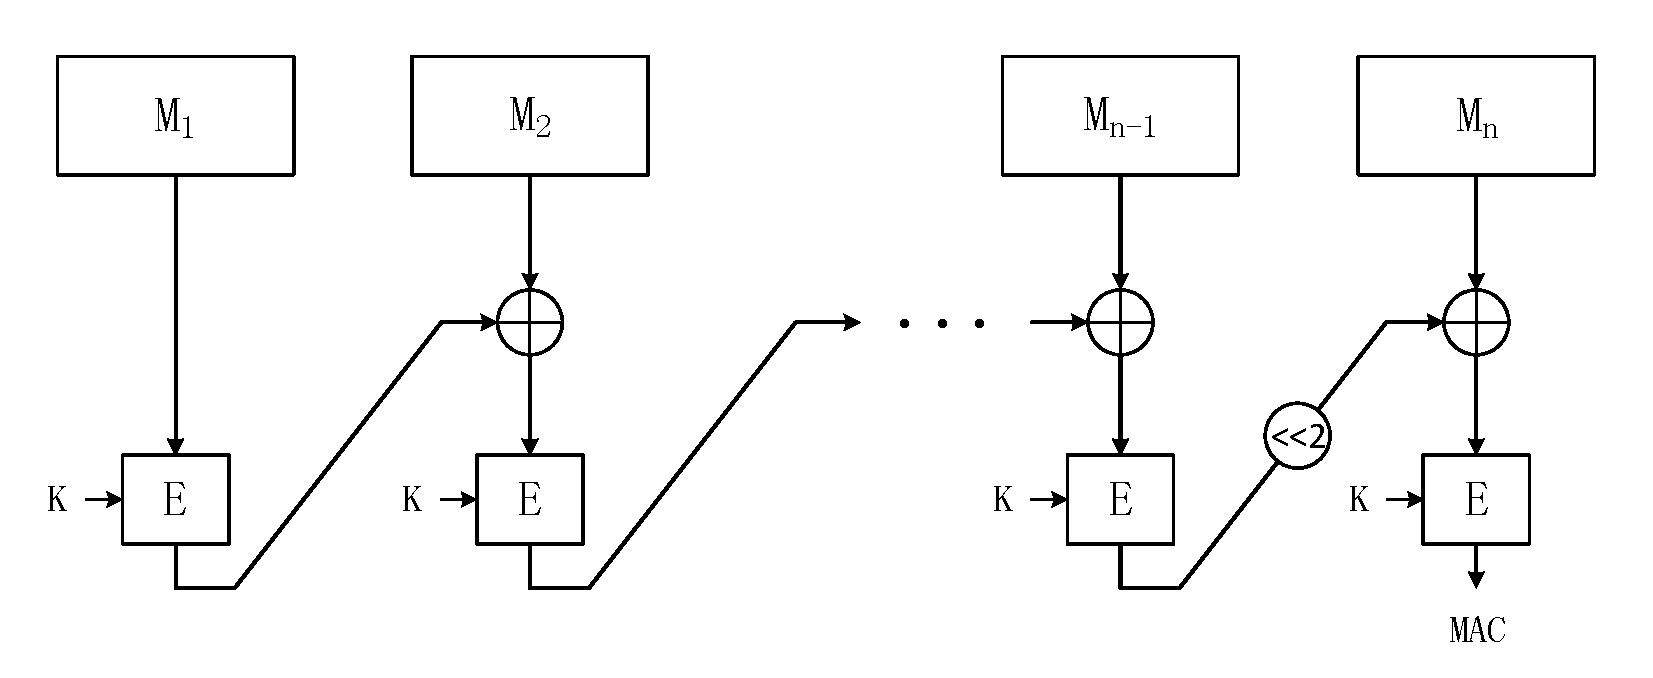
\includegraphics[width=5in]{scbc}
  \caption{SCBC-MAC方案}
  \label{fig:scbc}
\end{figure}

通过对消息$M$进行填充$M\| 1\|0^t$,使得消息M可以表示为$M=(M_1\|M_2\| \cdots \| M_n)\in (\{0,1\}^l)^n,l\geq 2$。我们的SCBC-MAC方案计算MAC可以表示如下:
\begin{equation}\label{scbc}
  SCBC_K(M)=E_K(E_K(\cdots E_K(E_K(M_1)\oplus M_2) \cdots)\ll 2 \oplus M_n)
\end{equation}

我们通过在最后一个消息块进行XOR运算之前,增加了一个左移2位的操作,这样简单的调整有效阻止了长度扩展攻击。SCBC-MAC的算法可以表示为算法~\ref{alg:scbc-mac}:

\begin{algorithm}[htbp]
  \caption{SCBC-MAC}
  \label{alg:scbc-mac}
  \begin{algorithmic}[1]
    \REQUIRE 输入消息$\mathbf{M}$,认证密钥$\mathbf{K}$,\\
            分组密码$E:k\times \{0,1\}^n \rightarrow \{0,1\}^n$
    \ENSURE 消息认证码
    \STATE $M \leftarrow M\| 1\|0^t$,将M填充为$l$的整数倍
    \IF{$l\geq 2$}
        \STATE 将消息M分隔为$M_1,M_2,\cdots,M_n$
    \ENDIF
    \STATE $y_0\leftarrow 0^l$
    \FOR{$i=1$ to $n-1$}
        \STATE $y_i \leftarrow y_{i-1}\oplus E_K(M_i)$
    \ENDFOR
    \STATE $y_n \leftarrow E_K(y_{n-1}\ll 2 \oplus E_K(M_n))$
    \RETURN $y_n$
  \end{algorithmic}
\end{algorithm}


\section{本章小结}
本章主要完成了密钥分配方案和消息认证码的设计。针对数据认证中的密钥分配需求,我们设计实现了基于单向hash链的密钥分配方案。对于报文传输阶段中使用的消息认证码,我们介绍了多种MAC方案,并针对我们的数据认证机制需求设计了SCBC-MAC方案。

\chapter{仿真实验与结果分析}
在第三章中我们设计实现了多跳长路径上多节点联合数据认证机制,第三章中提出了对多节点联合数据机制的优化方案,并对它们进行了理论分析。在本章中我们将使用仿真实验平台,对数据认证机制进行实验验证,并对它们的性能进行比较分析。6.1节介绍实验平台的环境,及相关仿真软件的介绍。6.2节是多跳长路径上多节点联合数据认证仿真实验及结果分析。6.3节是数据认证优化方案仿真实验及结果分析。
\section{实验平台环境}
\subsection{仿真实验环境}
为了搭建无线传感网的仿真环境,本文采用了仿真平台OMNeT++(Objective Modular Network testbed in C++)进行仿真,在Windows 7 的主机中安装的版本为OMNeT++4.6b1。 主机的配置为:
\begin{compactitem}
  \item DDR3内存,容量8G,频率1600MHz
  \item Core 双核处理器,主频2.6GHz
\end{compactitem}

现在进行网络仿真的工具很多,还有有NS2、NS3、OPNET、TOSSIM、GloMoSim和PowerTOSSIM等平台。NS2和NS3平台虽然有丰富的协议库支持,但是仿真时数据量过大,对复杂的无线传感网场景的仿真不合适,而且学习曲线比较高。OPNET平台要实现无线传感网仿真,学习门槛较高,而且其最大问题是提供的类库太少,仿真速度慢。TOSSIM、GloMoSim和PowerTOSSIM等其他仿真平台也有相应的局限性。

本文的实验中,我们选择了OMNeT++ 平台,OMNeT++是面向对象的离散事件仿真工具。OMNeT++基于Eclipse平台构建,是一款开源的仿真集成环境,由建模工具、仿真运行工具和输出结果分析工具等组成。OMNeT++还有INET、INETMANET或MIXIM等类库支持网络仿真,利用这些开源的包,很容易对各种网络协议进行仿真实验。

在OMNeT++中,主要使用C++语言创建仿真对象类,并使用ned文件配置仿真的参数,一个OMNeT++的仿真模型包括如下部分:
\begin{enumerate}\setlength{\itemsep}{-\itemsep}
  \item 网络拓扑结构描述文件(.ned文件):使用ned文件对仿真网络中的信道、门、连接和模块等进行配置。
  \item 消息或包定义文件(.msg文件):对网络中传输的消息或者数据报文进行定义,OMNeT++会自动从.msg生成相应的消息类。
  \item 模块描述文件(.h和.cc文件):使用C++语言描述模型中的各个模块。
\end{enumerate}
仿真模型使用C++编译器将.ned网络拓扑结构描述文件、.msg消息或包定义文件以及模块描述文件进行编译后,同仿真内核库以及用户接口库进行链接,生成可执行的仿真程序。OMNeT++不同于其他仿真平台,生成的仿真程序可以运行于没有安装OMNeT++的机器上。

\subsection{数据认证仿真框架}
下面将对搭建的无线传感网数据认证仿真模型进行介绍,
在我们的无线传感网数据认证机制研究中,我们的仿真模型主要包括两种对象:传感器节点和基站。
在本文中,我们假设所有的传感器节点均为相同的配置,部署时的能量相同。

\subsubsection{模块配置}
在OMNeT++仿真平台中,使用ned文件配置相应的模块,
传感器节点的配置文件如下所示,节点包括了一个输入输出门向量:
\begin{lstlisting}[language=C]
simple Node
{
    parameters:
        double txRate @unit(bps);
        double radioDelay @unit(s);       // 时间片
        volatile double iaTime @unit(s);  // 数据包发送间隔时间
        @display("i=device/wsn");
    gates:
        inout out;
}
\end{lstlisting}
基站的配置文件如下所示,基站也包括一个输入输出门向量,仿真实验中假设基站的通信不会受信道冲突的影响:
\begin{lstlisting}[language=C]
simple Bs
{
    parameters:
        @display("i=device/antennatower_l");
    gates:
        inout bsRadio[];
}
\end{lstlisting}
\subsubsection{模块类实现}
在我们的仿真实验中,传感器节点模块和基站模块都使用C++编写,我们对两个模块的实现做简要的介绍。

传感器节点使用了固定时间间隔内随机生成数据报文的方式仿真数据采集的过程,并采用自消息完成数据传输给簇头的过程,其采集过程函数表示如下:
\begin{lstlisting}[language=C]
void Node::initialize() {
    char msgname[20];
    sprintf(msgname, "event sensor # %d", getIndex());
    startEvent = new cMessage(msgname);
    iaTime = &par("iaTime");
    radioDelay = par("radioDelay");
    //事件捕获后的发送时间
    simtime_t t = simTime() + iaTime->doubleValue();
    if (ev.isGUI())
        getDisplayString().setTagArg("t", 2, "#808000");
    scheduleAt(t, startEvent);
}
\end{lstlisting}

传感器节点仿真发送数据包的过程主要由函数handleMessage完成:
\begin{lstlisting}[language=C]
void Node::handleMessage(cMessage* msg) {
    int src = getIndex();
    char msgname[40];
    sprintf(msgname, "event from cluster node %d", src);
    PacketCn *pkt = new PacketCn(msgname);
    pkt->setBitLength(952);
    pkt->setSource(src);
    pkt->setEvent(event);
    WATCH(pkt);
    //下一个事件发送时间,形成一个包传送给BS
    simtime_t tt = simTime() + iaTime->doubleValue();
    simtime_t nextTime=0;
    if((ceil(simTime()/radioDelay)*radioDelay)<tt)
        nextTime = tt;
    else
        nextTime = tt+radioDelay;
    ev << "send packet:"<<pkt<<" when "<<nextTime<< endl;
    send(pkt, "out$o");
    scheduleAt(nextTime, startEvent);
}
\end{lstlisting}

基站模块主要是接收数据报文,并对报文中的XMAC进行认证,确定报文的身份,其主要函数如下:
\begin{lstlisting}[language=C]
void Bs::handleMessage(cMessage* msg) {
    PacketCh *pkt = check_and_cast<PacketCh *>(msg);
    int event=pkt->getEvent();
    //计算event的XMAC
    int eventMac=this->Xmac(event);
    if(pkt->getXmac()==eventMac){
        ev<<"event received!"<<endl;
    }
    else{
        ev<<"trash packet!"<<endl;
    }
    delete pkt;
}
\end{lstlisting}

\section{仿真实验与方案评估}
在本节中我们对第三章和第四章中提出的数据认证方案进行仿真实验,并对它们的安全性能和能量开销进行分析评价。

我们的仿真条件是将1000个无线传感器节点部署到$150\times 100 m^2$大小的平面监测区域中,使用OMNeT++中的协议栈开源包在无线传感网中完成建簇过程,每个节点簇大小为$10 \times 10 m^2$,并完成传输路径的建立。每个传感器节点具有相同的硬件配置和通信能力,且每个节点的初始化能量为$1J$。在节点间的单跳通信中,发送1 字节报文需要$16.25 \mu J$能量,接收1字节报文需要$12.5 \mu J$ 能量,报文的大小为$24 byte$,报文中的每个MAC大小为$1 byte$。在每个节点进行认证时,计算一个MAC 需要的能量为$15 \mu J$。


\subsection{多跳长路径上多节点联合数据认证仿真实验}
在对多跳长路径上多节点联合数据认证机制(Multi Node Authentication,简称MNA方案)的仿真实验中,基站能够在初始化阶段通过每个部署节点的位置信息以及分配的ID建立多跳长路径。在各个簇与基站之间的路径上,通过HELLO报文和ACK报文完成上下行相关节点的发现,节点保存上下行相关节点的ID信息并建立共享密钥。

在实验中,每个簇内节点在一定的时间片内随机产生一个采集信息消息发送给簇头节点,当簇头节点收集到一定数量的采集信息消息以后进行数据聚合并发送数据报文给基站,当整个传感网中产生1000个数据报文时,实验结束,实验流程如图~\ref{fig:MPAtest}所示:
\begin{figure}[htbp]
  \centering
  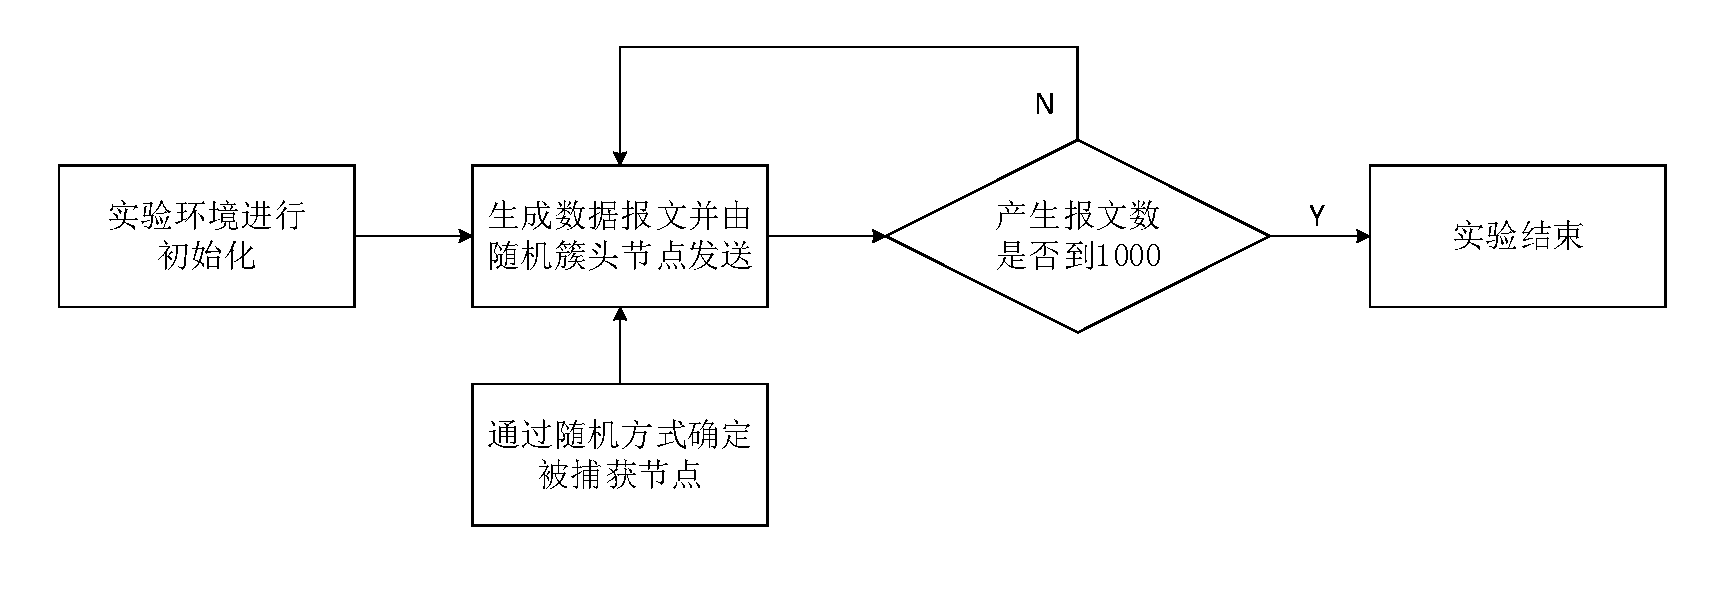
\includegraphics[width=6in]{MPAtest}
  \caption{多跳长路径上多节点联合数据认证仿真实验}
  \label{fig:MPAtest}
\end{figure}

每个节点都有一定的概率$p$被攻击而成为妥协节点,产生的1000个数据报文中既包括合法报文,也包括非法报文。网络中产生的非法数据报文的比例(Fabricated Reports Rate,简称FRR)是实验中被控制的变量,在不同的FRR下,我们进行仿真实验,并对结果进行分析。

如图~\ref{fig:MNAfilter}所示,是多跳长路径上多节点联合数据认证机制在参数$t=3$和$t=7$时路径中过滤比例同FRR的关系。横坐标是非法数据报文的比例FRR,纵坐标是路径中被丢弃的报文的比例。
仿真实验的结果表明我们的多跳长路径上多节点联合数据认证机制对虚假数据报文有较高的检测性能,大部分的虚假数据报文在路径中过滤阶段被丢弃。
由于仿真实验中,每个节点都有一定的概率$p$被攻击,因此路径中传输的虚假数据报文有可能因为攻击者利用多个被攻击节点合谋而绕过数据认证机制,最终被传输到基站。
可以看到在参数$t=3$,也就是簇规模较小时,相对$t=7$有更高的检测效率,我们的多节点联合数据认证机制在簇规模较小的无线传感网中有更好的安全性能。
\begin{figure}[htbp]
  \centering
  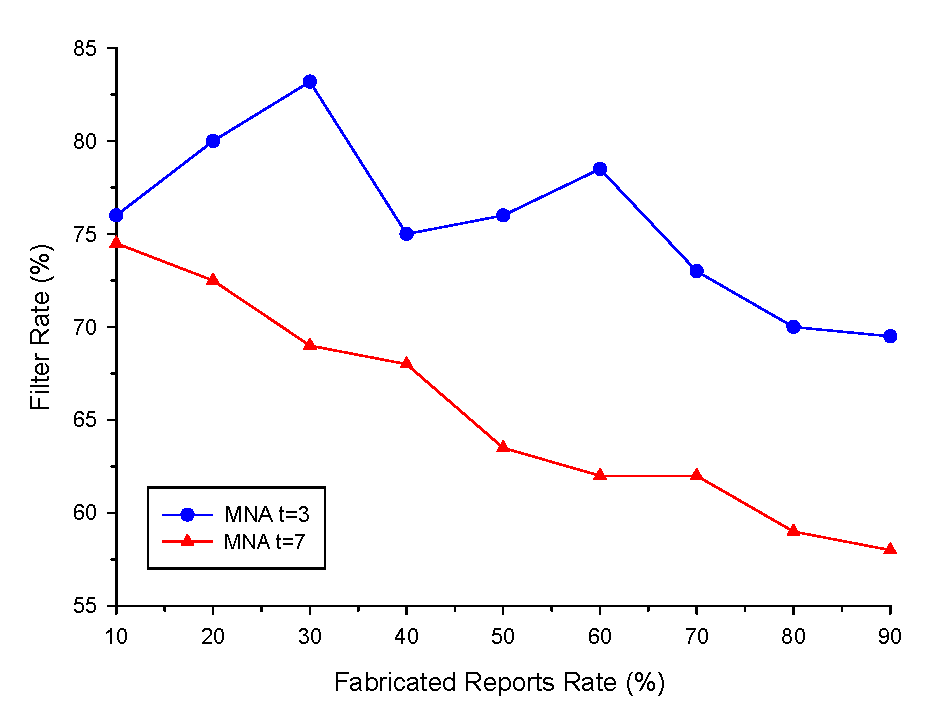
\includegraphics[width=5in]{MNAfilter}
  \caption{多节点联合认证的安全性能}
  \label{fig:MNAfilter}
\end{figure}

如图~\ref{fig:MNAenergy}所示,是多跳长路径上多节点联合数据认证机制在参数$t=3$和$t=7$时的能量开销,纵坐标是无线传感网中的总能量开销。可以从图中看出,能量开销随FRR的变大,基本是线性变化,因为当FRR变大时,有更多的报文在路径检测过程中被丢弃,减小了整个无线传感网中发送接收数据报文以及进行MAC计算完成认证的能量开销。在FRR较低时,簇规模对能量开销的影响不大,但是随着FRR的变大,簇规模较小的传感网比簇规模较大的传感网有更少的能量开销。

\begin{figure}[htbp]
  \centering
  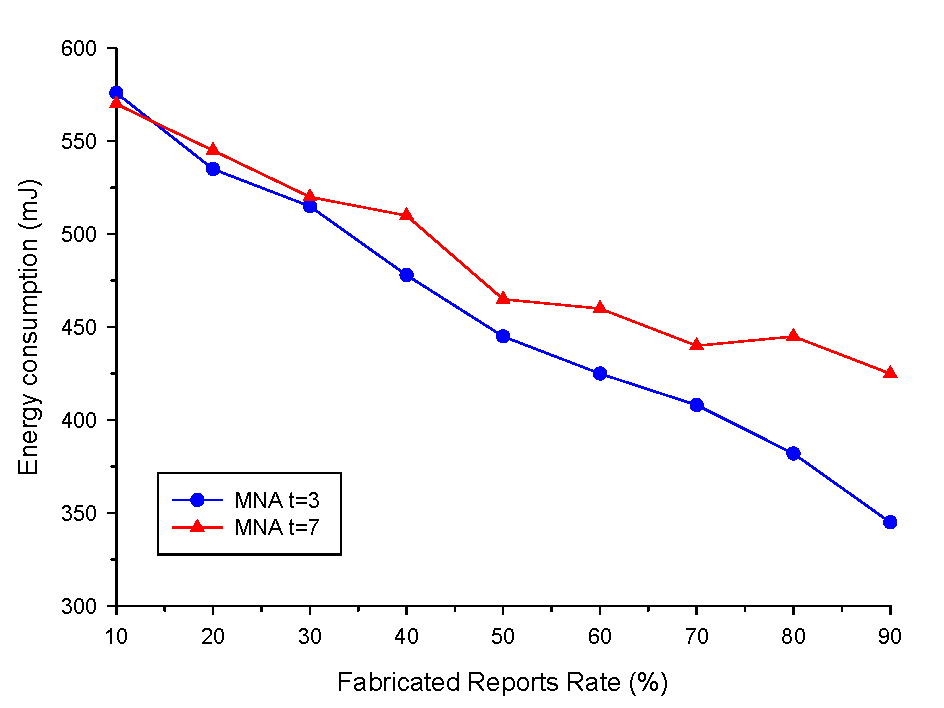
\includegraphics[width=5in]{MNAenergy}
  \caption{多节点联合认证的能量开销}
  \label{fig:MNAenergy}
\end{figure}

\subsection{数据认证优化方案仿真实验}
在对第四章提出的数据认证优化方案进行仿真实验时,实验条件与多跳长路径上多节点联合数据认证仿真实验相同。
\subsubsection{多路径抗节点失效机制的仿真实验}
为了增强数据认证机制的稳定性,在节点被攻击时保证数据认证机制的有效性,我们在4.1节提出了多路径抗节点失效的认证机制
(Multi Path Authentication,简称MPA)。

在初始化和密钥分配阶段,建立传输路径并完成上下行相关关系发现。在仿真实验中,利用相关机制建立两条备用不相交路径,以及两条编织路径。在实验中,每个簇内节点在一定的时间片内随机产生一个采集信息消息发送给簇头节点,当簇头节点收集到一定数量的采集信息消息以后进行数据聚合并发送数据报文给基站,当整个传感网中产生1000个数据报文时,实验结束。在对多路径抗节点失效机制进行仿真实验时,我们的无线传感网簇规模固定为$t=3$。

如图~\ref{fig:MPAfilter}所示,是多路径抗节点失效机制的路径中过滤比例同FRR的关系。在路径中检测率上,MPA方案相比MNA方案有较大的提升,而且MPA方案有更好的稳定性,在FRR变化时,MPA方案有比较稳定的检测率。
\begin{figure}[htbp]
  \centering
  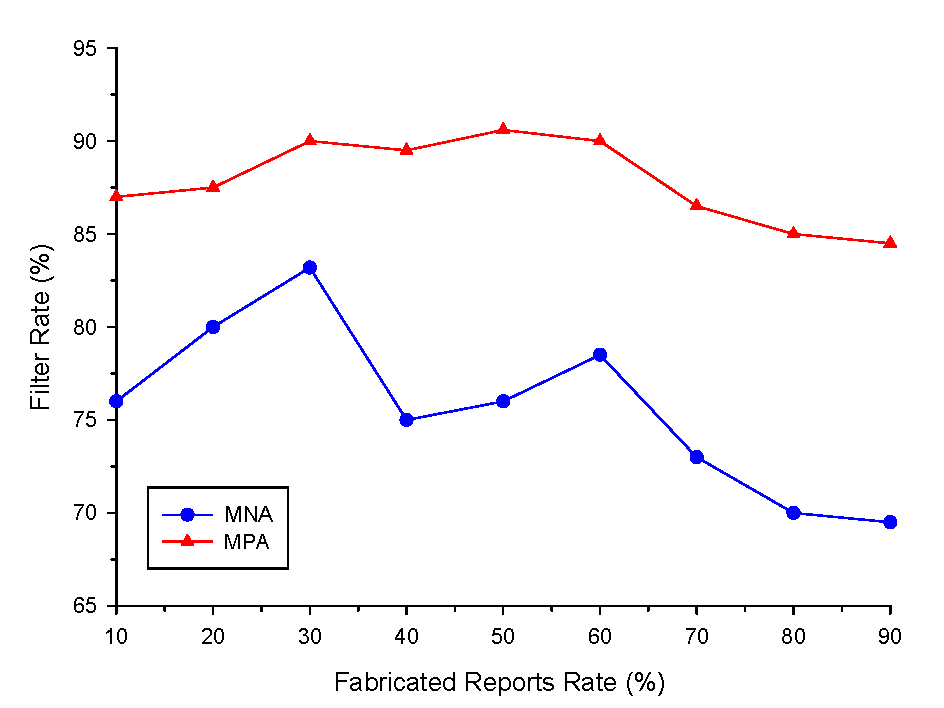
\includegraphics[width=5in]{MPAfilter}
  \caption{多路径抗节点失效机制的安全性能}
  \label{fig:MPAfilter}
\end{figure}

如图~\ref{fig:MPAenergy}所示,是多路径抗节点失效机制的能量开销。MPA方案和MNA方案的能量开销比较相近,在FRR较小时,由于MPA方案需要维护多条备用路径和编织路径,而且需要额外的hash函数运算,有更高的能量开销。随着FRR的变大,由于路径中检测率相比MNA 方案更高,虚假数据报文能更快的被丢弃,MPA方案的能量开销开始优于MNA方案。
\begin{figure}[htbp]
  \centering
  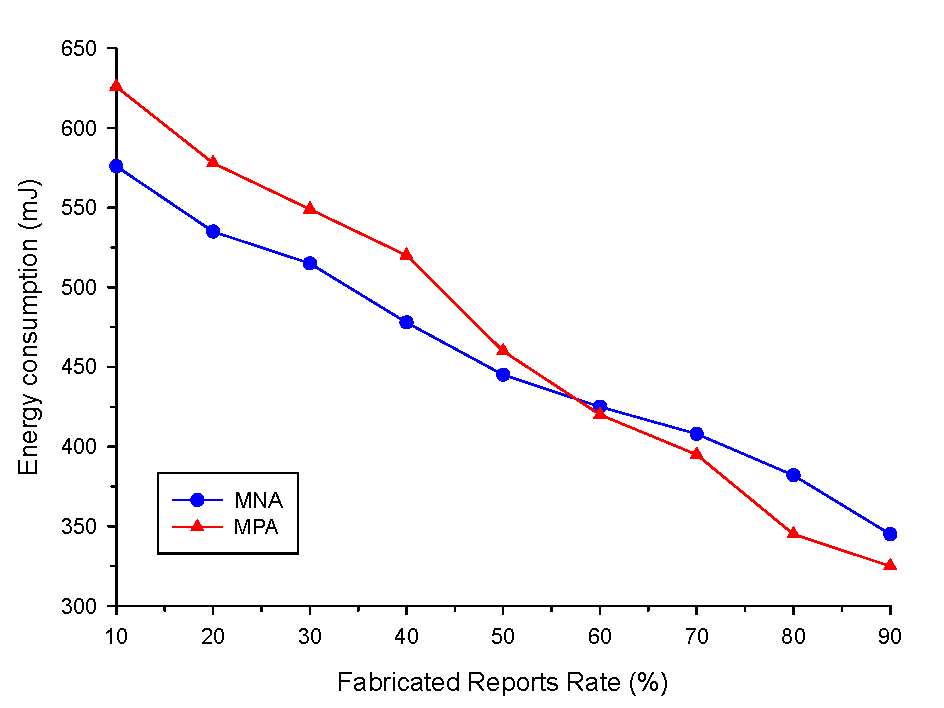
\includegraphics[width=5in]{MPAenergy}
  \caption{多路径抗节点失效机制的能量开销}
  \label{fig:MPAenergy}
\end{figure}


\subsubsection{动态步长数据认证机制的仿真实验}
为了在传感器网络节点受攻击影响较小的时候,压缩所传输的报文,降低节点能量消耗,我们在4.2节提出了动态步长多节点联合数据认证机制(Dynamic Step Authentication,简称DSA)。

进行动态步长数据认证机制的仿真实验时,整个网络的配置与多路径抗节点失效机制的仿真实验相同,但是不再建立备用路径和编织路径。在仿真过程中,基站对收到的报文进行统计,如果连续收到$\varphi = 3$条通过认证的数据报文,则进行步长调整,压缩数据报文的大小,节约节点的传输能量。

如图~\ref{fig:DSAfilter}所示,是动态步长数据认证机制的路径中过滤比例同FRR的关系。图中数据显示DSA方案同MNA方案在路径中检测率上没有明显差别,有相近的安全性能。
\begin{figure}[htbp]
  \centering
  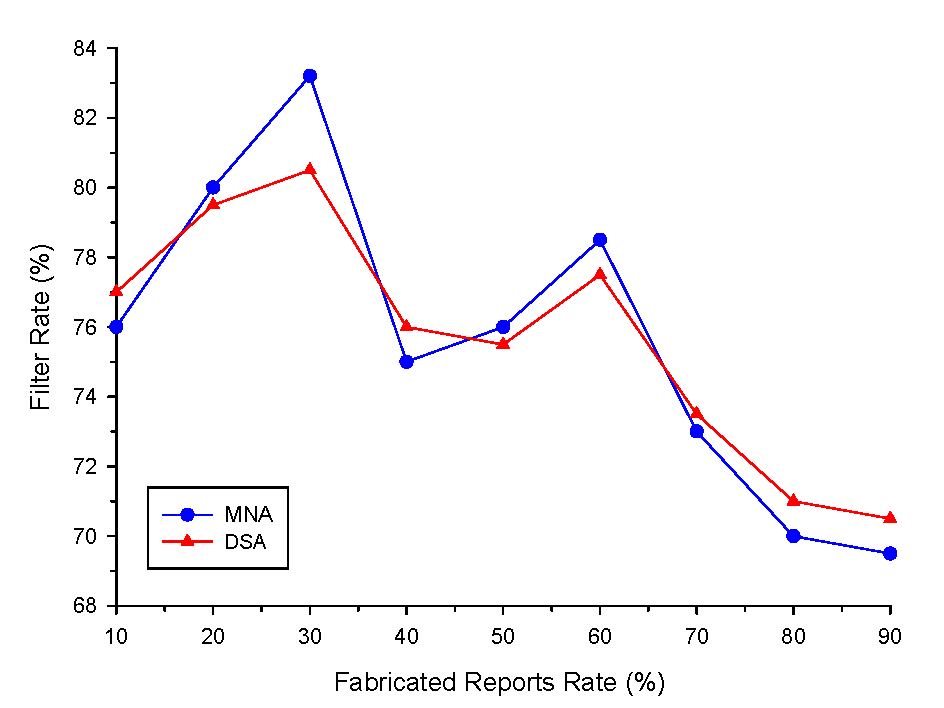
\includegraphics[width=5in]{DSAfilter}
  \caption{动态步长数据认证机制的安全性能}
  \label{fig:DSAfilter}
\end{figure}

如图~\ref{fig:DSAenergy}所示,是动态步长数据认证机制的能量开销。DSA方案相对MNA方案有较大的能量开销优化,尤其在FRR较小时,优化幅度较大。但是在FRR较大时,由于基站对网络安全状况的判定较低,无法维持步长的调整,压缩数据报文大小,因而能量开销的优化效果不明显。
\begin{figure}[htbp]
  \centering
  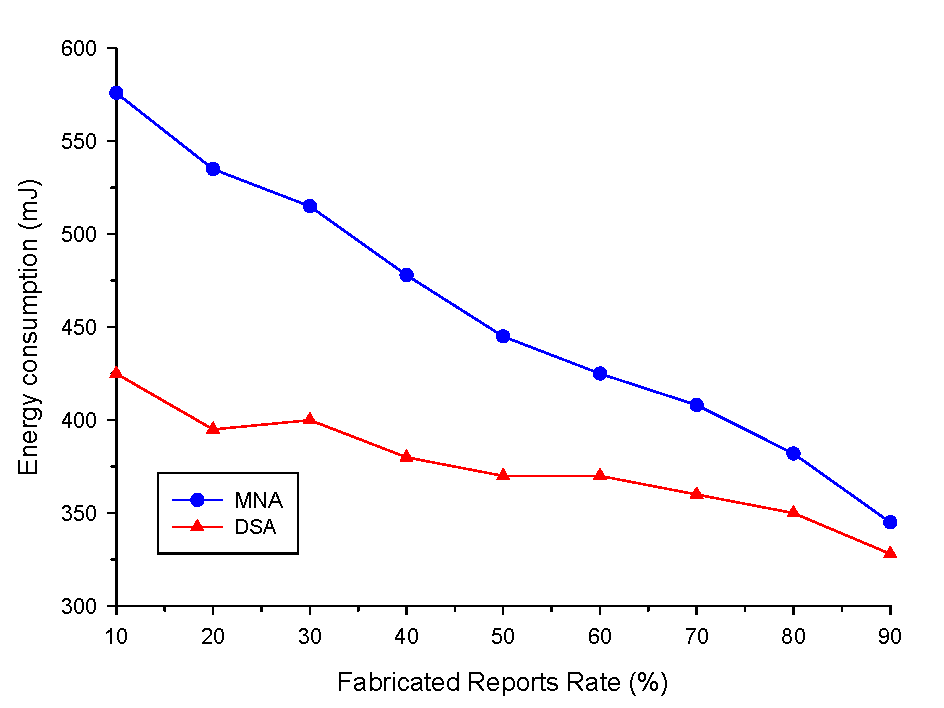
\includegraphics[width=5in]{DSAenergy}
  \caption{动态步长数据认证机制的能量开销}
  \label{fig:DSAenergy}
\end{figure}


\section{本章小结}
本章首先介绍了仿真实验环境的搭建,对使用OMNeT++进行无线传感网的仿真进行了介绍,对相关实验的框架搭建进行了说明。使用OMNeT++平台对我们的多跳长路径上多节点联合的数据认证机制进行仿真实验,验证该数据认证方案有较好的安全性能。
我们还对两个优化方案进行了仿真,实验结果表明两个方案分别对路径中检测率和通信开销有较好的改进。

\chapter{总结与展望}
本章对本文完成的研究工作进行总结,针对课题研究中待完善的地方,提出下一步工作的设想。
\section{本文总结}
无线传感网在许多大范围监测领域都有广泛的应用,在环境监测、军事侦察等领域都有规模化的应用。无线传感器节点通常被部署在
环境恶劣的无人值守区域,容易节点受损或者节点受攻击,导致传感网的传输受到严重影响。因此需要对无线传感网中的传输进行认证,保证数据传输的安全性。但是由于无线传感器节点计算能力、存储空间有限,而且节点能量受到限制,因此安全机制的设计必须满足轻量级的要求,以适应传感器节点的限制。我们设计了多跳长路径上多节点联合的数据认证机制,有效利用了数据认证机制保障了传输路径上的安全。

本文主要工作总结如下:
\begin{enumerate}\setlength{\itemsep}{-\itemsep}
  \item 深入研究了无线传感网中数据认证及其密钥分配的理论,分析了它们的发展研究现状,分析了数据认证在无线传感网中的应用,并总结了各种方案的优点和宝贵经验。
  \item 提出了多跳长路径上多节点联合数据认证的模型,设计实现了多跳长路径上多节
        点联合数据认证协议,并设计了路径上节点关系的维护算法,对协议的安全
        性能进行了分析评价。
  \item 针对多跳长路径上多写点联合数据认证协议的不足,对算法进行了优化,提
        出了多路径抗节点失效机制和动态步长多节点联合数据认证机制,并对优化
        方案的安全性能进行了分析评价。
  \item 围绕多跳长路径多节点联合数据认证机制的需求,对密钥分配方案进行了深
        入研究,提出了基于单向 hash 链的密钥分配方案,并对认证中的 MAC 进行
        了研究,提出了适应数据认证机制需求的 MAC 码。
  \item 通过仿真实验验证了本文中提出的方案的安全性能以及优化效果。
\end{enumerate}



\section{未来工作于展望}
本文设计实现的多跳长路径上多节点联合的数据认证机制能够很好地提升了无线传感网数据传输的安全性,取得了一定的成果。但是由于无线传感网本身的复杂性以及部署场景的多样性,我们的机制对不同工作场景下的无线传感网的适应性还需进一步研究,在数据认证的具体算法以及密钥分配等方向还有进一步研究的空间。结合现阶段以及完成的工作,我们未来可做的相关工作有:

\begin{enumerate}\setlength{\itemsep}{-\itemsep}
  \item 本文研究的数据认证机制与无线传感网现有的各层次协议结合还不够,在后续的工作中可以将数据认证机制同其他协议结合起来,例如同网络层的路由协议相结合,将数据认证的相关报文使用路由报文发送。
  \item 针对本文的数据认证机制提出的两个优化方案,虽然在仿真实验环境中已经进行了验证,但在实际的规模化无线传感网中部署比较复杂,可进一步通过搭建真实的传感器节点平台和较大规模无线传感网环境,对相关方案进行针对性的优化。
  \item 密钥分配方案的设计实现还不够完善,需要对相关的算法进行进一步的改进,形成完整的密钥管理机制,并对密钥分配方案的效率和安全性进行分析评价。使用的单向hash函数还有改进的空间,可以进一步压缩其计算开销。
\end{enumerate}






%\chapter{相关研究概述}
无线传感网在环境监测、工业控制、资源监测和军事侦察等领域都有重要的应用,具有非常良好的前景。但是区别于传统的网络,无线传感器节点一般都部署在无人值守的环境恶劣地区或敌对区域,可能受到敌人的攻击破坏,所以安全问题十分突出。同时由于无线传感器节点的存储空间和计算能力的限制,安全机制的复杂性受到约束,因此设计适合无线传感网应用需求的安全机制十分重要。

本章首先对无线传感网的安全技术进行概述,然后对无线传感网的认证机制及其密钥分配方案进行概述。

\section{无线传感网安全技术概述}
无线传感网的节点一般部署在无人值守区域,使得无线传感网的安全问题尤为突出,特别是在军事侦察等应用领域。无线传感网不能直接沿用传统无线网络的安全机制,设计无线传感网的安全机制时,必须考虑到无线传感器网的如下限制
\upcite{c1:limitation}:
\begin{compactitem}
  \item 节点的存储空间、计算能力和通信能力有限,特别是节点的能量有限,严重制约了安全机制的发展。
  \item 无线传感网有无线自组网的缺点,缺乏基础设施建设,节点之间使用不安全的无线通信。
  \item 部署的位置一般是敌对区域或者危险区域,节点很容易受到物理攻击或者破坏。
\end{compactitem}

无线传感网的应用决定了其安全目标与传统网络有所不同,更侧重于保护感知的数据,保证数据的安全。
在无线传感网中,安全技术的目标主要包括\upcite{c1:attack}:
\begin{compactitem}
  \item 数据认证:通过认证确保数据来自经过身份认证的节点,保证数据的安全。
  \item 数据保密:确保只有通过认证的节点才能获取消息中的内容,不会暴露保密的内容。
  \item 数据完整性:确保所有受到的消息没有被未经授权的设备所篡改。
  \item 可用性:确保传感器节点在受到攻击时仍然能提供指定的基本服务。
  \item 数据新鲜:保证数据在指定时间内到达目的节点,确保数据的有效性。
\end{compactitem}

\subsection{无线传感网面临的安全威胁}

无线传感网的协议栈包括传输层、网络层、链路层和物理层,各层都会遭到不同的攻击。对于各层的攻击,有各种防御手段来保护无线传感网的安全,传输层主要研究认证机制及面向认证的密钥管理技术,网络层主要研究路由安全协议,数据链路层主要研究数据帧的安全传输,物理层主要研究节点间通信信道安全。
无线传感网中常见的攻击与防御措施\upcite{c1:attack}如表~\ref{tb:wsnattack}所示:

\begin{table}[htbp]
  \centering
  \caption{无线传感网常见的攻击与防御措施}
  \label{tb:wsnattack}
  \begin{minipage}[t]{0.8\textwidth}
    \begin{tabularx}{\linewidth}{|c|c|X|}
      \hline
%      \multirow{1}*{网络层次}
%        & 常见的攻击 & 防范措施\\
      \multirow{1}*{网络层次}  & \multicolumn{1}{c|}{常见的攻击} & \multicolumn{1}{c|}{防范措施}\\
      \hline
      \multirow{2}*{传输层}
        & 泛洪攻击 & 用户询问 \\\cline{2-3}
        & 同步破坏攻击 & 认证机制 \\
      \hline
      \multirow{7}*{网络层}
        & 泛洪攻击 & 广播和组播半径限制 \\\cline{2-3}
        & 黑洞攻击 & 节点身份认证,冗余路径 \\\cline{2-3}
        & 错误定向攻击 & 数据帧转发签名 \\\cline{2-3}
        & 蠕虫洞攻击 & 基于信任等级的路由 \\\cline{2-3}
        & 创建路由环 & 篡改校验、认证 \\\cline{2-3}
        & 汇聚节点攻击 & 加密、逐跳认证机制 \\\cline{2-3}
        & 虚假路由攻击 & 冗余机制、数据一致性检测 \\
      \hline
      \multirow{3}*{数据链路层}
        & 资源耗尽攻击 & 限制通信速度,竞争门限控制 \\\cline{2-3}
        & 碰撞攻击 & 纠错校验码 \\\cline{2-3}
        & 非公平竞争攻击 & 使用非优先级策略 \\
      \hline
      \multirow{3}*{物理层}
        & 拥塞攻击 & 使用优先级消息、宽频通信、间歇通信 \\\cline{2-3}
        & 无线干扰 & 变频通信、跳频通信 \\\cline{2-3}
        & 物理破坏 & 节点伪装和隐藏 \\
      \hline
    \end{tabularx}\\[2pt]
  \end{minipage}
\end{table}

物理层受到的攻击主要包括拥塞攻击、无线干扰和物理破坏。拥塞攻击是物理层最常见的攻击,Xu 等就提出了4种不同的拥塞攻击方法\upcite{c1:jamming},能够使无线传感网停止工作。无线干扰是干扰传感器节点的通信信道,和拥塞攻击一样都能严重影响节点的数据发送和接收。通过物理攻击,篡改节点信息是物理层的另一种攻击方法,攻击者能获得节点的内存信息,包括密钥和加密数据,从而破坏该节点的工作。

数据链路层容易受到碰撞攻击,攻击者利用协议的漏洞,在无线传感网发送大量的干扰数据包,与正常数据包传输发生碰撞,造成无线传感网正常数据无法传输,并且消耗节点能量。数据链路层还容易受到资源耗尽攻击,即向特定节点发送大量数据,消耗其节点能量,使之失效。非公平竞争是指攻击者通过发送高优先级的数据包,在网络中一直占据通信信道,使得正常节点一直无法使用信道,无法发送数据。

在无线传感网中,大量的传感器节点部署在监测区域内,报文需要经过多跳才能到达基站,无线传感网的特性决定了它没有固定的拓扑结构,所以每个节点都能进行路由,因此攻击者可以利用该特点发动网络层攻击。网络层受到的攻击包括泛洪攻击、黑洞攻击、错误定向攻击、蠕虫洞攻击、创建路由环攻击、汇聚节点攻击和虚假路由攻击。

传输层受到的攻击包括泛洪攻击和同步破坏攻击。当攻击者发送大量的连接请求,就能严重影响到无线传感网的通信,甚至无法进行正常网络通信,也就是泛洪攻击。同步破坏攻击是指向建立了通信连接的节点不断发送伪造的发送失败消息,使节点一直因为帧丢失而进行重传,而且达到攻击传感器网络的目的。

无线传感网各个协议栈都容易受到攻击,虽然都有相应的防御的措施,但是现阶段的安全机制方案还不够完善,严重制约了无线传感网的应用和发展。


\subsection{无线传感网现有的安全技术}

无线传感网面临着多种攻击的威胁,许多安全技术方案在保护其安全方面已经有了突破。
对于无线传感网的安全技术,在保证数据传输安全的前提下,其设计要考虑到如下需求:
\begin{compactitem}
  \item 稳定性:整个无线传感网的安全体系不会因为个别节点的失效或者被攻击而瘫痪。
  \item 可扩展性:传感网加入新节点,不会对原有的安全体系造成影响,同时不应产生过大的计算开销。
  \item 灵活性:安全技术不能影响到网络的部署结构的灵活性。
  \item 低开销:安全技术的计算开销、通信开销和存储开销应当适合无线传感器节点的能力,不会影响到节点的正常功能。
\end{compactitem}


无线传感网现有的安全技术主要包括加密算法、安全路由、数据聚合、入侵检测、认证机制和密钥管理,其中认证机制和密钥管理将在2.2节与2.3节进行详细论述。

\subsubsection{密码算法}
由于无线传感器节点自身的局限性,计算能力和节点存储空间有限,导致目前非对称密码算法在传感器节点不能直接应用。而对称密码算法需要的计算能力更小,存储空间开销也相对较小,因而目前的传感器网络主要使用的是对称密码算法。如RC5\upcite{c1:RC5}、RC6\upcite{c1:RC6}、Camellia\upcite{c1:Camellia}、TEA\upcite{c1:TEA} 和MISTY1\upcite{c1:MISTY1}等对称加密应用在无线传感网中,在文献\cite{c1:encryptionCompare}中,Law等对这些对称加密算法在无线传感器节点中的运行性能进行了比较和分析。

虽然现阶段非对称密码还很少应用在无线传感网的安全协议中,但是随着硬件技术的进步,传感器节点的计算和存储能力不断提高,低开销的非对称密码算法应用在无线传感网的安全协议中成为了可能,也成为了现阶段无线传感网密码算法研究的热点。现阶段非对称密码在传感器节点上的尝试主要是基于椭圆曲线的密码算法(ECC),David等将ECC应用在TinyOS中
\upcite{c1:EC},Gura等将ECC和RSA在MICA上成功实现\upcite{c1:ECC},并对它们进行了分析比较。
\subsubsection{安全路由}
路由技术在传统的网络中有非常成熟的协议,但是由于无线传感网的特性,没有特定的路由节点,每个节点都要完成路由的功能,导致无线传感网的路由技术与传统网络有较大区别。现阶段多数路由协议都注重提高路由效率,以降低节点的能量消耗,但是这样也造成了潜在的安全问题。

许多相关研究都针对无线传感网的路由安全问题进行了探索,如Deepak等提出的多路由机制\upcite{c1:multiroute},通过在多条路径上传输同一个数据报文,来防御选择性转发攻击,但是该方案中,数据报文需要传输多次,造成通信开销的浪费。还有其他路由协议通过加密和认证等方法提高路由的安全性能,如Karlof等人的方案\upcite{c1:Karlof03}和Li等人的方案
\upcite{c1:Li}。
\subsubsection{数据聚合}
数据聚合减少了无线传感网中的冗余数据,降低了通信开销,节约了节点能量。通过数据聚合安全机制,提高了无线传感网中数据私密性,提高了网络传输的安全性。

Priyanka等人在数据聚合中添加了错误数据检测机制,提出了一种高效的数据聚合方案\upcite{c1:Priyanka},保证了数据的安全传输。类似的研究还有Suat等人的方案\upcite{c1:suat},通过将数据聚合和安全传输以及错误报文过滤相结合,提高了无线传感网数据传输的安全。

Sivagami等人提出的方案\upcite{c1:Sivagami} 中,通过多节点对之间延迟发送消息认证码来对发送的数据进行认证,实现了安全的数据聚合,并且降低了传输开销。

Zhu等人提出了一种错误数据报文过滤机制\upcite{c1:zhu},通过节点间的交叉认证,保证了错误报文在被捕获节点不超过设计参数的情况下会在路径中被过滤。

\subsubsection{入侵检测}
当无线传感器节点的部署在敌对区域时,很容易受到攻击,节点被捕获或者受损不可避免,而攻击者可以通过这些妥协节点发送进一步的攻击,从而影响整个无线传感网的安全。因此在无线传感网中,入侵检测技术可以发现网络中的异常情况,并识别恶意节点,成为了无线传感网的重要安全技术手段。入侵检测主要通过对传感网中的数据发送行为和数据报文进行分析,发现异常事件,并确定恶意行为的来源节点。

无线传感网的入侵检测机制主要由入侵检测、入侵跟踪和入侵相应3部分构成。在Wang等人提出的方案中\upcite{c1:wang},构建了覆盖可疑节点及其相邻节点的支配树,通过同可疑节点的相邻节点进行合作,来判断可疑节点是失效节点或者是恶意节点,并通过使用基于覆盖的启发式技术来提升检测效率。

恶意节点检测方案还有Mathews等人的检测方案\upcite{c4:mathews2007detecting},Zhang等人提出的基于位置的妥协节点检测机制\upcite{c1:zhang},以及Agah等提出的基于非合作博弈的入侵检测方案\upcite{c1:Agah}。

\section{无线传感网认证机制概述}
无线传感网的核心功能是在目标区域采集数据,并将数据传输到数据中心。攻击者通常会针对部分节点进行攻击,在捕获节点以后,利用这些节点联合对整个无线传感网进行攻击,因此认证机制在保证无线传感网数据安全传输中发挥重要作用。认证机制按照不同的方法,可以分为对称密钥和非对称密钥认证机制、消息认证和身份认证机制或广播认证和单播认证机制。在本节中,主要讨论无线传感网的数据认证和身份认证。

\subsection{无线传感网数据认证概述}
无线传感网的数据认证有基于对称密钥和基于非对称密钥两种,因为节点的性能限制,基于对称密钥的数据认证在无线传感网中应用还不多,现阶段的方案主要是基于对称密钥实现。

现阶段的数据认证方案主要是Perrig等人提出的$\mu TESLA$方案\upcite{c1:Tesla},以及一系列基于$\mu TESLA$的改进方案。
\begin{figure}[htbp]
  \centering
  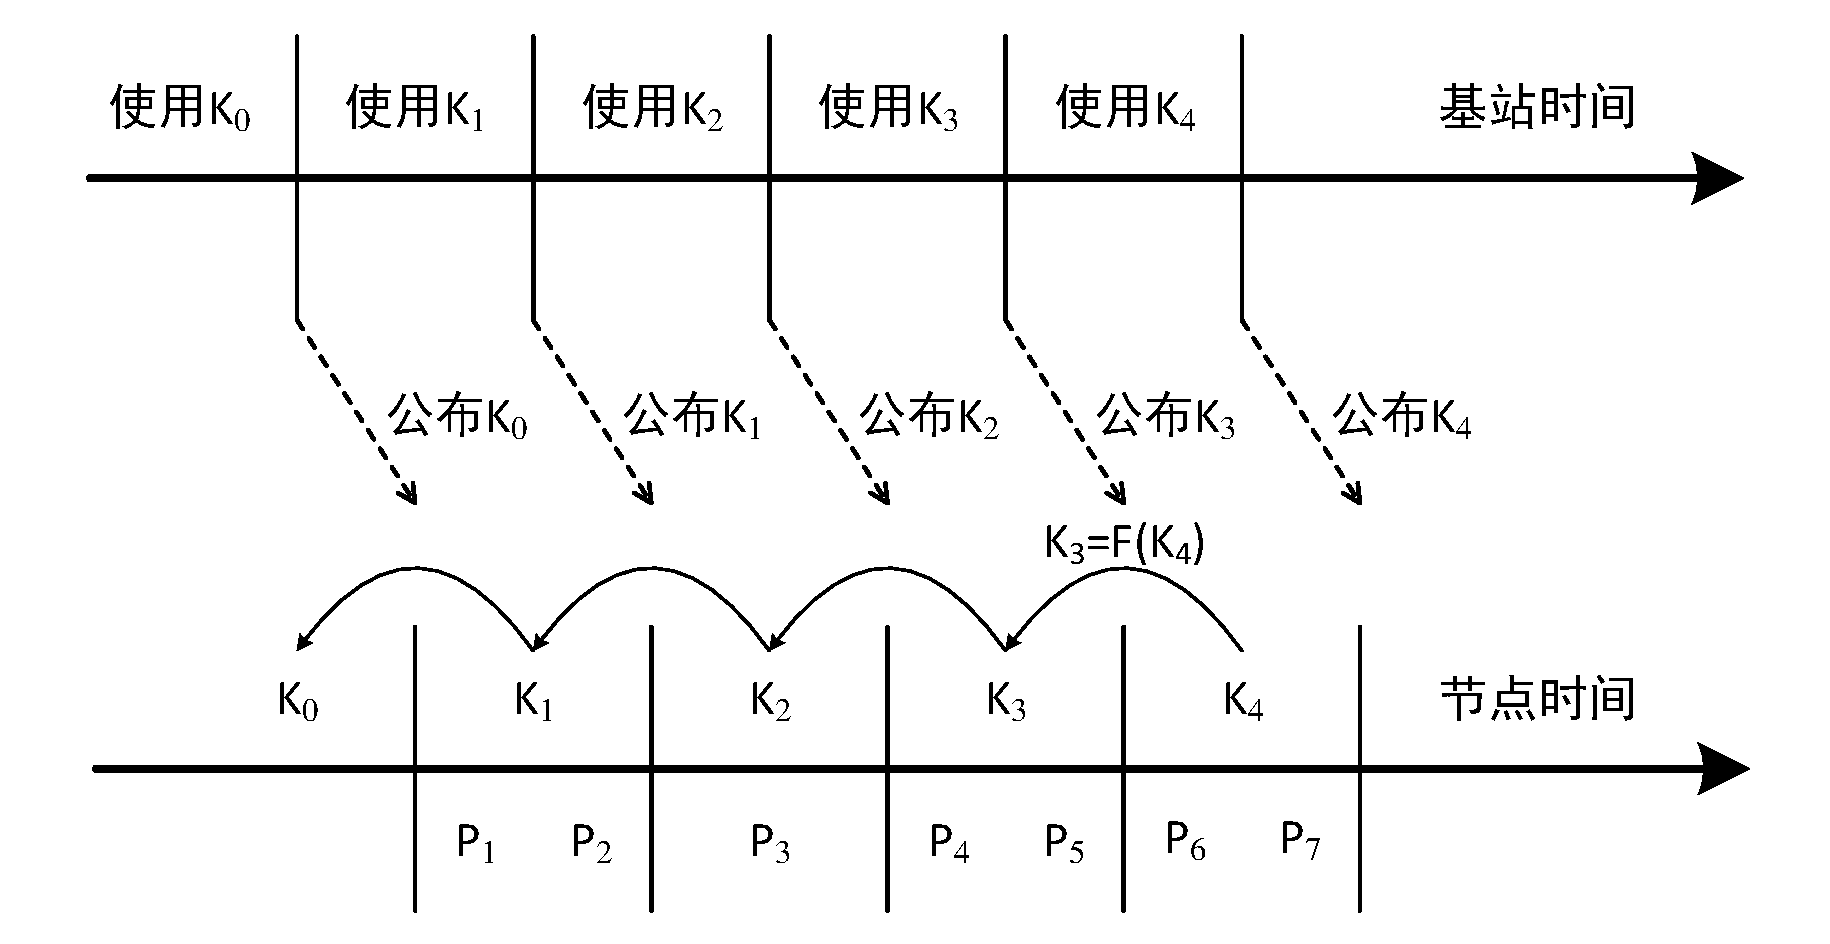
\includegraphics[width=5in]{TESLA}
  \caption{$\mu TESLA$认证机制}
  \label{fig:TESLA}
\end{figure}
如图~\ref{fig:TESLA}所示,是$\mu TESLA$方案的认证过程,$\mu TESLA$是基于对称密钥的,对报文计算消息认证码的认证密钥和节点对报文进行认证的密钥是相同的。其认证过程包括密钥建立、广播报文、自举接收者和对报文认证等步骤。其中密钥分发是通过单向hash 函数F 来实现的,如$K_3=F(K_4)$。 然后广播一个密钥$K_i$加密后的报文,无线传感网中基站和节点采用不同的时隙,使广播加密报文和接收到相应的密钥不同步。通过延迟发布密钥$K_i$,使得认证过程具有非对称性,提高认证的安全性能。通过比较报文的接收时间和认证密钥发布的时隙,能对报文的安全性进行检查。但该方案仍有其缺点:密钥的发布延后于报文的到达,因此节点接收到的报文必须缓存在节点中,浪费节点宝贵的存储空间,并且有可能被攻击者发动泛洪攻击,大量的伪造报文填满传感器节点的缓存空间,导致无线传感网传输功能失效,攻击者也容易发动虫洞攻击,威胁传感网的安全。

Liu等人基于$\mu TESLA$方案,提出了多级$\mu TESLA$方案\upcite{c1:MultiTesla},采用多级密钥链解决$\mu TESLA$方案中密钥链占用存储空间过大,容易导致泛洪攻击的问题。该方案使用预装初始化参数的方案,代替$\mu TESLA$方案中通过单播进行初始化的过程。如图~\ref{fig:MultiTESLA},是多级$\mu TESLA$方案的认证过程。在该方案中,Liu使用了2级时间,在1级时间中,将时间划分为$n_0$个间隔,每个时间间隔对应该级的单向hash链中的密钥$K_i,1\leq i \leq n_0$,其中密钥还是同$\mu TESLA$ 方案,使用单向hash链生成。一个1级时间间隔又被划分为$n_1$个2级时间间隔,每个2级时间间隔的密钥使用
$K_i,1\leq i \leq n_0$作为密钥种子生成。每个2级时间间隔内发送的报文用对应的密钥进行认证,其中的密钥链头$K_i,0$ 在前一个1级时间发布。
\begin{figure}[htbp]
  \centering
  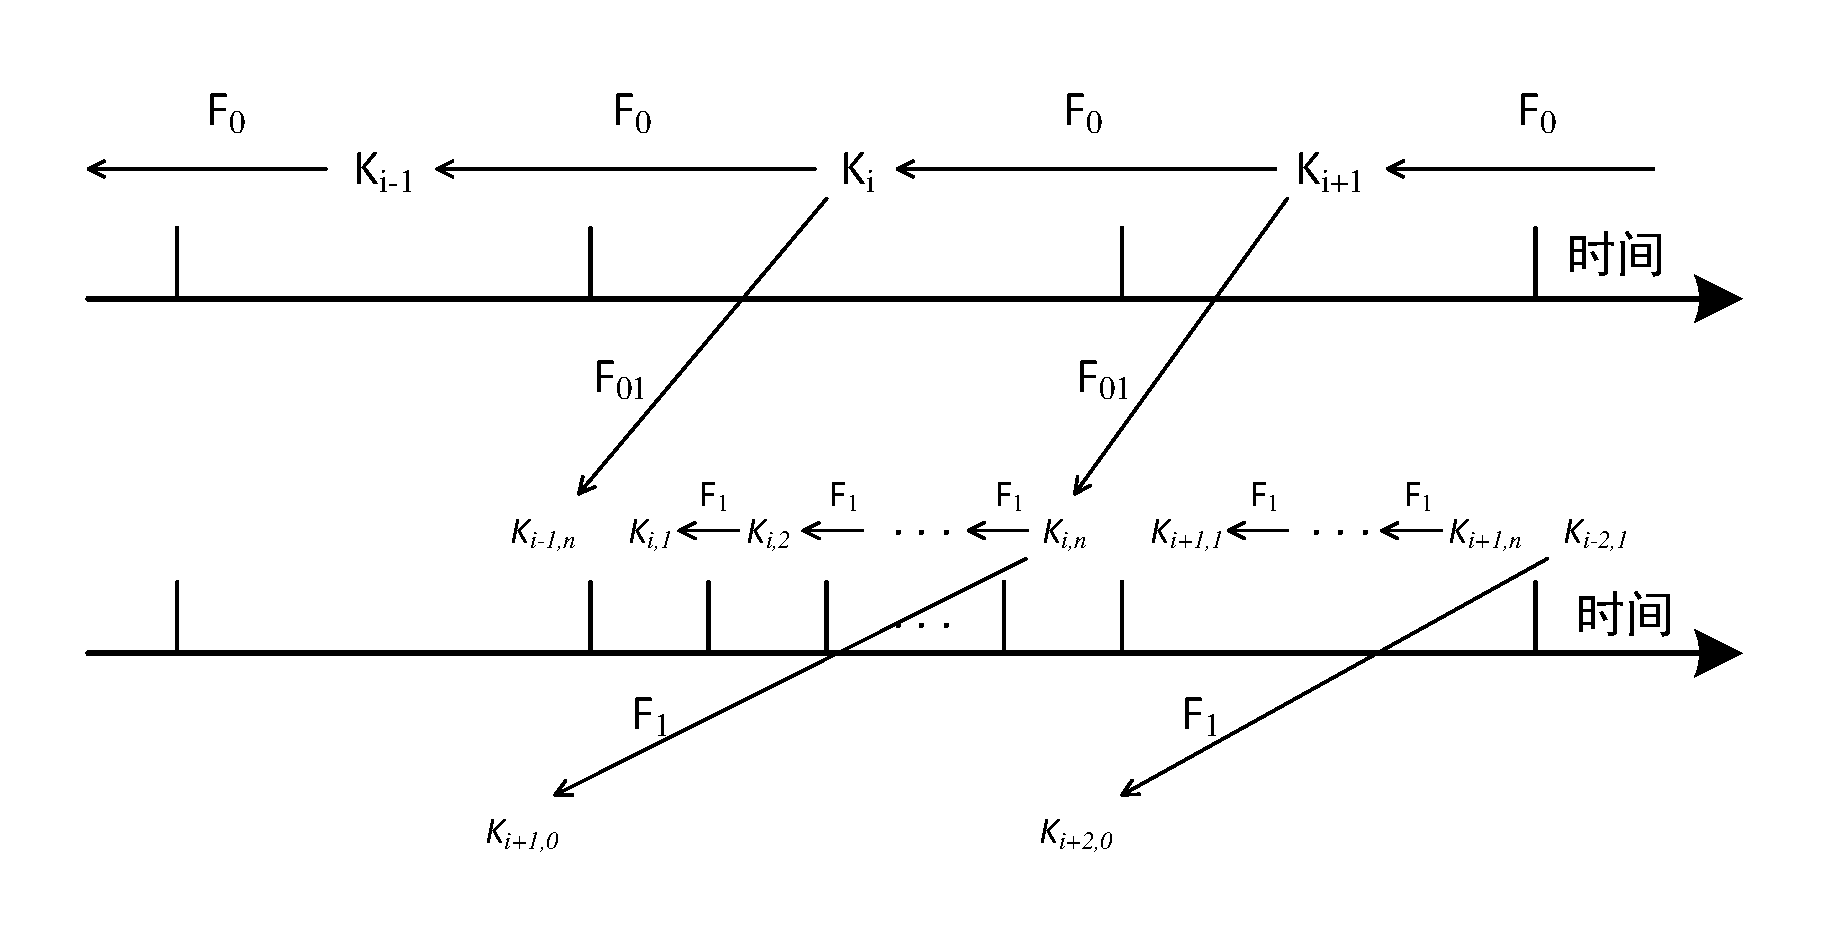
\includegraphics[width=5in]{multiTESLA}
  \caption{多级$\mu TESLA$认证机制}
  \label{fig:MultiTESLA}
\end{figure}

在裴庆祺等人的$\mu TESLA$改进方案中\upcite{c1:MMtesla},引入了$(t,n)$的门限秘密共享,每个认证密钥被分隔为$n$个密钥片,分配到各个基站。在无线传感网中执行原有的$\mu TESLA$方案,将密钥片进行广播,当一个节点接收到超过$t$个密钥片之后,就通过秘密共享的算法,对认证密钥进行恢复,重构出认证密钥。该方案提高了$\mu TESLA$方案的认证率,并且有高可靠性和高容忍性的特点,缺点是通信开销明显增加。

Anas等人提出了一种基于信任模型的认证方案\upcite{c1:anas},使用一个轻量级的基于椭圆曲线的简单认证密钥协议。通过通信实体之间建立信任级别,使非对称密钥认证系统能在资源有限的无线传感器节点上运行。

Dong等人利用消息预认证提出了一个基于密钥链的过滤方案\upcite{c1:verifyfilter},能对无线传感网中的广播进行过滤,有效减少虚假广播对传感网数据传输的影响,该方案的缺点是无法有效防御攻击者的联合节点攻击。




\subsection{无线传感网身份认证概述}

攻击者可以通过对网络发送大量的虚假数据报文,大量消耗节点的计算和存储能力,消耗节点的能量,导致传感网的失效。因此对传感网中的节点进行身份认证尤为重要。
文献\cite{c2:chan2003random}中,利用随机配对密钥分配方案,一个密钥仅会分配给一对节点,来实现一种非常简单的身份认证,即两个节点通过使用预分配的密钥对消息的加密和解密判断是否是经过认证的节点。但是该方案无法实现真正的身份认证,因为被捕获的节点可以伪装成正常节点进行欺骗,对无线传感网进行攻击。

现有的身份认证方案主要有非对称密钥认证和秘密共享认证。
由于无线传感器节点的限制,现阶段非对称密钥认证的实现一般是消耗能量较多的计算由基站完成,消耗能量较少的计算由节点完成。秘密共享的认证则是基于多个节点共同对一个节点进行认证。

虽然现阶段由于传感器节点的限制,非对称密钥没有被广泛应用于无线传感网的认证,但是许多研究也对此进行了探索。
在非对称密钥机制中,椭圆曲线密码(Elliptic Curve Cryptography,ECC)是一种轻量级的方案,研究结果表明,160位的ECC 能获得相当于1024位RSA密码的安全性能。而且使用非对称密钥不需要$\mu TESLA$方案中的延迟发布密钥,还能提高认证系统的安全性。

Watro等人提出了一个基于RSA算法的认证机制TinyPK\upcite{c1:Watro},该方案使用请求-应答机制。
该方案使用了双重校验,来保证认证机制的安全性。
当一个节点需要同另一个节点进行认证时,向该节点发送一个请求信息,其中包括两部分。第一部分是使用认证中心的私钥进行签名的请求节点的公钥,第二部分是使用请求节点私钥签名的时间戳和消息认证码。应答节点接收到该请求消息以后,使用认证中心的公钥对第一部分进行解密,获取请求节点的公钥。使用请求节点的公钥解密第二部分,获得时间戳和消息认证码,通过时间戳和消息认证码的校验,来判断请求节点的合法性。如果通过,则建立两个节点之间的安全通信。

在Bauer等人的方案\upcite{c1:Bauer}中,使用了秘密共享的思想进行身份认证。当一个节点请求对另一个节点的认证时,应答节点发送消息给认证中心,宣告自己被请求做认证处理,处理中心将请求节点的私钥进行划分,将秘密片广播给应答节点的邻居节点,所有节点发回给认证中心一个判定消息,如果通过认证的消息超过阈值,则请求节点通过认证,应答节点此时与认证中心进行交互,更新自己的私钥。

现有的身份认证方案还有Benenson提出的基于ECC的方案\upcite{c1:Benenson},Cao等基于vBNN-IBS提出的多用户广播认证方案\upcite{c1:Cao}。



\section{无线传感网密钥分配方案概述}

\subsection{无线传感网密钥分配概述}
无线传感网的密钥分配是其安全技术研究的一个重要内容,包括密钥预分发、共享密钥发现等研究方向。

无线传感网中的密钥分配与传统无线网络有较大区别,在传统的无线网络中,密钥分配方案的研究已经取得了许多成果,但是由于无法适应无线传感网的特点,这些成果无法应用于无线传感网中。因为WSN节点资源的限制,传统无线网络中节点计算开销和通信开销较大的密钥分配方案无法适用。在设计无线传感网的密钥分配方案时,不仅要保证方案的安全性能,也要权衡计算开销和通信开销。

进行认证的基础是密钥分配,设计一个面向无线传感网需求的密钥分配方案,才能保证认证机制的性能。
\subsection{无线传感网密钥分配方案分类}
近些年来,WSN的密钥分配有了许多新的研究成果,根据所适用的密钥是否是对称密钥,可以将方案分为对称密钥方案和非对称密钥方案。随着传感器技术的发展,非对称密钥技术可能成为将来无线传感器密钥分配的主流,但是由于目前无线传感器节点的计算能力和存储空间的限制,现有的无线传感网密钥分配以对称密钥方案为主。基于对称密钥,有很多的密钥分配机制的研究成果,表~\ref{tb:wsnkey}列出了目前无线传感网主要的密钥分配方案:

\begin{table}[htbp]
  \centering
  \caption{无线传感网主要的密钥分配方案}
  \label{tb:wsnkey}
  \begin{minipage}[t]{0.8\textwidth}
    \begin{tabularx}{\linewidth}{|c|X|X|}
      \hline
%      \multirow{1}*{网络层次}
%        & 常见的攻击 & 防范措施\\
      \multirow{1}*{数学结构}  & \multicolumn{1}{c|}{密钥分配方案} & \multicolumn{1}{c|}{密钥分配方法} \\
      \hline
      \multirow{3}*{密钥池}
        & E-G方案 & 随机预分发 \\\cline{2-2}
        & q-composite方案 & \\\cline{2-3}
        & PIKE方案 & 基于网格预分发\\
      \hline
      \multirow{4}*{二元对称多项式}
        & Blundo方案 & 确定预分发\\\cline{2-3}
        & Liu-Ning方案 & 基于随机子集预分发 \\\cline{2-3}
        & GBKP方案 & 基于网格预分发 \\\cline{2-3}
        & CPKS方案 & 基于位置预分发 \\
      \hline
      \multirow{2}*{MDS 码生成矩阵}
        & Blom方案 & 确定预分发 \\\cline{2-3}
        & Du-Deng方案 & 基于随机子集预分发 \\
      \hline
      \multirow{2}*{区组}
        & Camtepe方案 & 组合设计 \\\cline{2-3}
        & Camtepe混合组合设计方案 & 组合设计及随机预分发 \\
      \hline
    \end{tabularx}\\[2pt]
  \end{minipage}
\end{table}



\subsection{无线传感网典型密钥分配方案概述}
根据密钥分配方法的不同,我们对不同类别的无线传感网密钥分配方案进行概述:
\subsubsection{基于随机预分发的密钥分配}
Eschenauer和Gligor基于随机图理论,提出了无线传感网中随机密钥预分配的方案\upcite{c2:Eschenauer2002}(简称E-G方案),该方案包括3个阶段。在密钥预分发阶段,密钥分发中心生成一个足够大的密钥池$P$,然后对于每个传感器节点,从中随机选择$m$个不同的密钥,形成一个密钥环,并将密钥保存到传感器节点的存储空间中。在密钥发现阶段,每个节点通过相邻节点发现机制寻找物理上相邻的节点,由于所有节点的密钥是从密钥池中随机取出的,相邻节点可能存在相同的密钥,如果相邻节点存在共享密钥,则作为两者之间的会话密钥。当相邻节点之间不存在共享密钥,则开始路径密钥建立阶段。通过在密钥发现阶段建立的节点连通图$G(V,E)$(V为传感器节点的顶点集合,E为有共享密钥的传感器节点之间构成的边集),在图中查找一条通往没有共享密钥的相邻节点的路径,建立相邻节点之间的路径密钥。

在E-G方案中,两个相邻节点之间有共享密钥的概率$p$同节点存储密钥数$m$之间的关系可以表示为:$p=1-\frac{((P-m)!)^2}{(P-2m)!P!}$。E-G 方案使得每个节点只需要存储较小数量的密钥,就可以有较高概率使得无线传感器网络完成密钥建立过程,符合无线传感网的特点要求。但是E-G 方案作为最早提出的无线传感网密钥预分发方案,也有自身的缺点,当妥协节点增多时,无法保证无线传感网的通信安全,因为节点不具备防篡改的机制。而且当一个节点被捕获时,节点上存储的密钥材料全部都暴露给了攻击者,而且这些密钥可能是其他节点间的会话密钥,也就是使攻击者能攻击其他节点之间的通信。

在E-G方案的基础上,有许多方案对随机密钥预分配进行了改进,提升随机密钥预分配机制的性能。
Chan等人在E-G方案的基础上提出了q-composite 随机密钥预分配方案\upcite{c2:chan2003random},每个节点从密钥池$P$中获取$m$个不同的密钥。方案的密钥个数阈值为$q$,当两个节点之间的共享密钥个数$q^{'}$满足$q^{'}> q$,则两个节点之间使用hash函数$K=hash(K_1\| K_2\| \cdots \| K_{q^{'}})$生成会话密钥,在q-composite方案中,hash函数使用了SHA-1\cite{c2:sha1}。q-composite保证了相邻节点之间的安全链路,密钥个数阈值增大时,链路的安全性能也增大。在无线传感网被捕获节点较少时,该方案节点间链路的安全性能比E-G方案更好,但是当被捕获节点增多时,该方案的安全性能明显下降。


在Blom的对称密钥生成方案\upcite{c2:Blom84} 基础上,Du等人将其与随机密钥预分发结合,提出了无线传感网多密钥空间密钥预分发方案\upcite{c2:du2005pairwise}。先使用Blom方案生成$\omega$个密钥空间,每个节点从中选择$\tau$个密钥空间保证在存储空间中$(2 \leq \tau \leq \omega)$,如果两个节点上存储了一个相同的密钥空间,则他们之间计算生成一个共享密钥。与E-G 方案和q-composite方案相比,Du-Deng方案通过计算适合的参数$\omega$和$\tau$,能明显提高抵抗链路攻击的性能,但是同时也增加了节点的计算开销。

Blundo利用二元对称多项式的性质,提出了节点对密钥建立方案\upcite{c2:Blundo1998}。密钥服务器随机生成一个有限域上的$k$ 阶二元对称多项式$f(x,y)=\sum _{i,j=0}^k a_{i,j} x^i y^j$,对于对称多项式,有$f(x,y)=f(y,x)$。对于任意节点$i$,服务器计算$f(i,y)$,然后将$k+1$个系数存入节点存储空间。当节点$i$和节点$j$需要建立对密钥时,计算$f(i,y)$ 在$y=j$ 时的值,计算$f(j,y)$在$y=i$时的值,因为$f(i,j)=f(j,i)$,所以$f(i,j)$就可以作为节点$i$和节点$j$之间的对密钥。

在Blundo方案的基础上,Liu-Ning提出了基于对称二元多项式池的随机密钥预分配方案\upcite{c2:liu2005establishing}。
密钥服务器在有限域$F_q$上随机生成一个二元对称多项式的集合$\phi=\{f_i(x,y),i=1,\cdots,t\}$,对于节点$i$,将子集$\phi_i\subseteq \phi$装入存储空间。当两个节点发现有相同的二元多项式,则直接使用Blundo的节点对密钥建立方案建立会话密钥。当被捕获的节点较少时,Liu-Ning方案有较好的安全性能,但是在攻击者捕获了较多节点,也就是获得较多二元多项式的时候,链路的安全性能相较E-G方案和q-composite方案更低。

利用节点的位置信息,Liu提出了最近对密钥方案(CPKS)\upcite{c2:LiuN03},节点实际分布位置在其期望分布位置周围服从均匀分布。每个节点与自己期望分布位置最近的$t$节点之间建立对密钥,例如,对节点$u$的相邻节点$v$,密钥服务器生成对密钥$K_{u,v}$,并将$u,K_{u,v}$和$v,K_{u,v}$分别存入节点$u$和节点$v$。通过两个节点之间的ID信息可以判断两个节点之间是否存在对密钥。在节点位置信息已知时,该方案相比前述方案有更好的性能,缺点是网络扩展性较差,加入新节点,需要大量节点能量消耗。

Du提出的基于部署知识的方案\upcite{c2:Du06} 中,将密钥池$S$划分为$t\times n$的子密钥池$S_{i,j}(1\leq i\leq t,1\leq j\leq n)$,子密钥空间$S_{i,j}$对应着部署组$G_{i,j}$。根据部署位置的信息,不同的子密钥池之间发现共享密钥。该方案提高了无线传感网中节点链路连通的概率,但是子密钥池的划分对安全性能的影响较大。


\subsubsection{基于网格预分发的密钥分配}
为了解决随机密钥预分配方案中链路密钥的不确定性,Liu提出了基于网格的密钥预分配方案(GBKP)\upcite{c2:LiuND08}。
对一个$m\times n$的传感网,如图~\ref{fig:GBKP}所示,$G_i$为部署分组。对$G_i$中的节点分配ID集合$\{(i-1)m+j|j=1,\cdots,m\}$,对$G_i^{'}$中的节点分配ID集合$\{i+(j-1)m|i=1,\cdots,n\}$。服务器生成$m+n$个对称二元多项式分配给每行每列,使得同一行或同一列的节点能直接生成对密钥,不同行或列的节点,通过中间节点生成链路密钥。
类似的基于网格预分发的密钥分配方案还有Chan 提出的PIKE方案\upcite{c2:ChanP05}。
\begin{figure}[htbp]
  \centering
  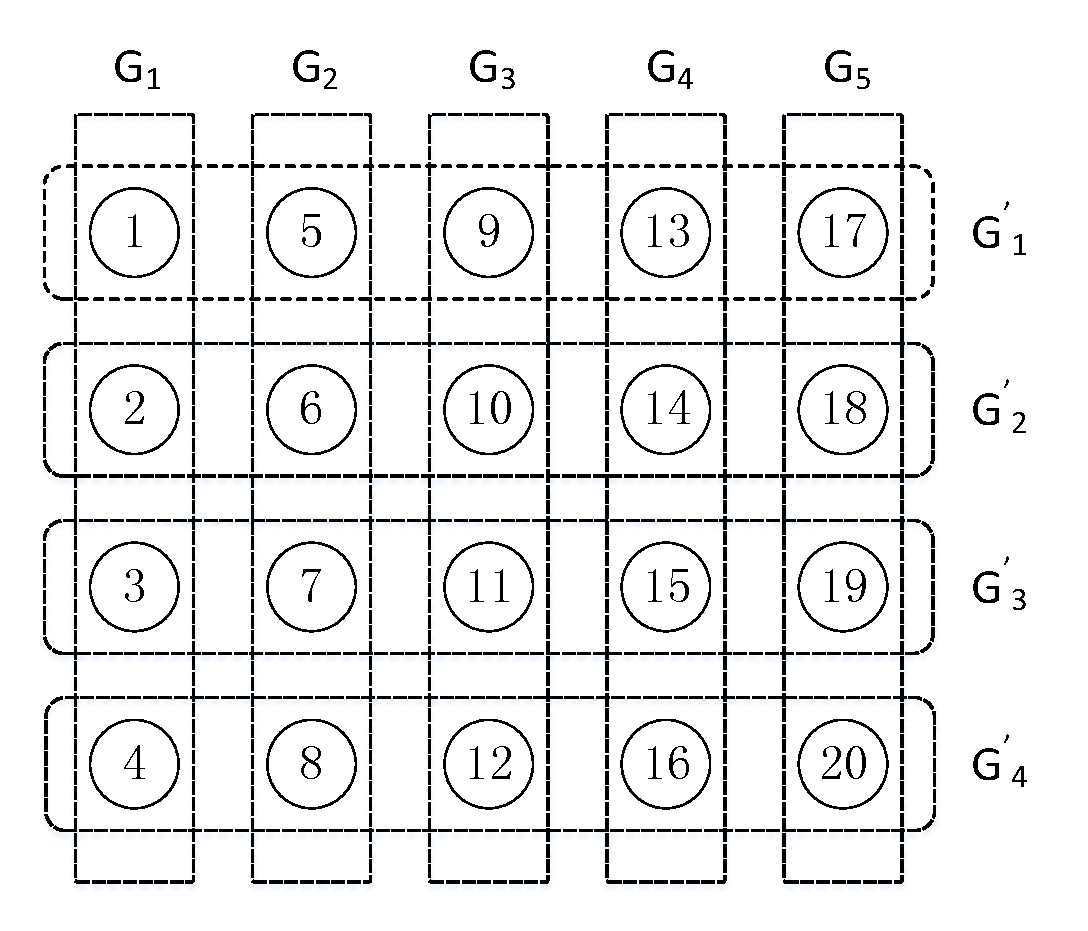
\includegraphics[width=4in]{GBKP}
  \caption{基于网格的密钥预分配方案}
  \label{fig:GBKP}
\end{figure}

\subsubsection{基于组合设计的密钥分配}
Camtepe把组合设计的理论应用于无线传感网的密钥分配\upcite{c2:CamtepeY07},使用组合设计理论来划分密钥池和密钥环。
对一个规模为$N$的无线传感网,生成一个对称BIBD,$(n^2+n+1,n+1,1)$,其中$n$为满足$n^2+n+1\geq N$的最小素数,密钥池的大小为$n^2+n+1$,密钥环的长度为$n+1$。这个方案保证了无线传感网中的任意一对节点有共享密钥,或通过中间节点生成的链路密钥。
为了解决该方案在网络规模方面的限制,Camtepe 还提出了组合设计与广义四边形想结合的方案。





%%% Local Variables:
%%% mode: latex
%%% TeX-master: "../main"
%%% End:

\begin{ack}
  衷心感谢导师 xxx 教授和 xxx 副教授对本人的精心指导。他们的言传身教将使我终生受益。

  感谢 \nudtpaper{},它的存在让我的论文写作轻松自在了许多,让我的论文格式规整漂亮了许多。

\end{ack}


\cleardoublepage
\phantomsection
\addcontentsline{toc}{chapter}{参考文献}
\bibliographystyle{bstutf8}
\bibliography{ref/refs}

\begin{resume}

  \section*{发表的学术论文} % 发表的和录用的合在一起

  \begin{enumerate}[{[}1{]}]
  \addtolength{\itemsep}{-.36\baselineskip}%缩小条目之间的间距,下面类似
  \item Zongxiao Lan,Geming Xia,Aolong Zhou. Communication cost optimized session key transmission scheme for WSN based on non-perfect secret sharing. ICITMI, 2014.
  \end{enumerate}

\end{resume}

% 最后,需要的话还要生成附录,全文随之结束。
\appendix
\backmatter
% TeX
\chapter{模板提供的希腊字母命令列表}

大写希腊字母:
\begin{table}[htbp]
\centering
\begin{tabular}{llll}
\toprule
$\Gamma$~\verb|\Gamma| & $\Lambda$~\verb|\Lambda| & $\Sigma$~\verb|\Sigma| & $\Psi$~\verb|\Psi| \\
$\Delta$~\verb|\Delta| & $\Xi$~\verb|\Xi| & $\Upsilon$~\verb|\Upsilon| & $\Omega$~\verb|\Omega| \\
$\Theta$~\verb|\Theta| & $\Pi$~\verb|\Pi| & $\Phi$~\verb|\Phi| & \\
\midrule
$\varGamma$~\verb|\varGamma| & $\varLambda$~\verb|\varLambda| & $\varSigma$~\verb|\varSigma| & $\varPsi$~\verb|\varPsi| \\
$\varDelta$~\verb|\varDelta| & $\varXi$~\verb|\varXi| & $\varUpsilon$~\verb|\varUpsilon| & $\varOmega$~\verb|\varOmega| \\
$\varTheta$~\verb|\varTheta| & $\varPi$~\verb|\varPi| & $\varPhi$~\verb|\varPhi| & \\
\bottomrule
\end{tabular}
\end{table}

小写希腊字母:
\begin{table}[htbp]
\centering
\begin{tabular}{llll}
\toprule
$\alpha$~\verb|\alpha| & $\theta$~\verb|\theta| & $o$~\verb|o| & $\tau$~\verb|\tau| \\ 
$\beta$~\verb|\beta| & $\vartheta$~\verb|\vartheta| & $\pi$~\verb|\pi| & $\upsilon$~\verb|\upsilon| \\ 
$\gamma$~\verb|\gamma| & $\iota$~\verb|\iota| & $\varpi$~\verb|\varpi| & $\phi$~\verb|\phi| \\ 
$\delta$~\verb|\delta| & $\kappa$~\verb|\kappa| & $\rho$~\verb|\rho| & $\varphi$~\verb|\varphi| \\ 
$\epsilon$~\verb|\epsilon| & $\lambda$~\verb|\lambda| & $\varrho$~\verb|\varrho| & $\chi$~\verb|\chi| \\ 
$\varepsilon$~\verb|\varepsilon| & $\mu$~\verb|\mu| & $\sigma$~\verb|\sigma| & $\psi$~\verb|\psi| \\ 
$\zeta$~\verb|\zeta| & $\nu$~\verb|\nu| & $\varsigma$~\verb|\varsigma| & $\omega$~\verb|\omega| \\ 
$\eta$~\verb|\eta| & $\xi$~\verb|\xi| & $\varkappa$~\verb|\varkappa| & $\digamma$~\verb|\digamma| \\ 
\midrule
$\upalpha$~\verb|\upalpha| & $\uptheta$~\verb|\uptheta| & $\mathrm{o}$~\verb|\mathrm{o}| & $\uptau$~\verb|\uptau| \\ 
$\upbeta$~\verb|\upbeta| & $\upvartheta$~\verb|\upvartheta| & $\uppi$~\verb|\uppi| & $\upupsilon$~\verb|\upupsilon| \\ 
$\upgamma$~\verb|\upgamma| & $\upiota$~\verb|\upiota| & $\upvarpi$~\verb|\upvarpi| & $\upphi$~\verb|\upphi| \\ 
$\updelta$~\verb|\updelta| & $\upkappa$~\verb|\upkappa| & $\uprho$~\verb|\uprho| & $\upvarphi$~\verb|\upvarphi| \\ 
$\upepsilon$~\verb|\upepsilon| & $\uplambda$~\verb|\uplambda| & $\upvarrho$~\verb|\upvarrho| & $\upchi$~\verb|\upchi| \\ 
$\upvarepsilon$~\verb|\upvarepsilon| & $\upmu$~\verb|\upmu| & $\upsigma$~\verb|\upsigma| & $\uppsi$~\verb|\uppsi| \\ 
$\upzeta$~\verb|\upzeta| & $\upnu$~\verb|\upnu| & $\upvarsigma$~\verb|\upvarsigma| & $\upomega$~\verb|\upomega| \\ 
$\upeta$~\verb|\upeta| & $\upxi$~\verb|\upxi| & & \\ 
\bottomrule
\end{tabular}
\end{table}

希腊字母属于数学符号类别,请用\verb|\bm|命令加粗,其余向量、矩阵可用\verb|\mathbf|。


\end{document}
